\documentclass[english]{tktltiki}
\usepackage[pdftex]{graphicx}
\usepackage{subfigure}
\usepackage{url}
\usepackage{float}
\usepackage{textcomp}
\usepackage{verbatim}
\usepackage{multirow}
\usepackage{fixltx2e}


\begin{document}


\onehalfspacing


\title{Using Blockchain Technology and Smart Contracts for Access Management in IoT devices}

\author{Rupsha Bagchi}
\renewcommand{\instructor}{\textbf{Instructor} : Prof. Sasu Tarkoma}
\renewcommand{\advisor}{\ \textbf{Advisor}  \, \ :  Oscar Novo}
\date{\today}
\maketitle

\numberofpagesinformation{\numberofpages\ pages + \numberofappendixpages\ appendices}
\classification{\protect{\ \\
C.2.0 [General]: Security and Protection,\\
C.2.4 [Distributed Systems]: Distributed applications,\\
C.3 [Special Purpose and Application-Based Systems],\\
C.4 [Performance of Systems]: Reliability, availability, and serviceability,\\
C.5.3 [Microcomputers]: Portable devices,\\
H.3.4 [Systems and Software]: Distributed Systems}}

\keywords{Internet of Things, Blockchain, Ethereum, Smart Contracts, Device Management, Docker }

\begin{abstract}

The Internet of Things is a proliferating industry, which is transforming many homes and businesses, making them smart. However, the rapid growth of these devices and the interactions between these devices, introduces many challenges including that of a secure management system for the identities and interactions of the devices. While the centralized model has worked well for many years, there is a risk of the servers becoming bottlenecks and a single point of failure, thereby making them vulnerable to Denial-of-service attacks. 

As a backbone of these interactions, Blockchain is capable of creating a highly secure, independent and distributed platform. Blockchain is a peer to peer, distributed ledger system that stores all the transactions taking place within the network. The main purpose of the servers that form a part of the distributed system is to provide a consensus, using various consensus algorithms, on the state of the blockchain at any given time and to store a copy of all the transactions taking place.

This thesis explores the Blockchain technology in general and investigates its potential with regard to access management of constrained devices. A proof of concept system has been designed and implemented that demonstrates a simplified access management system using Ethereum Blockchain. This was done to check whether the concept can be applied at a global level. Although the latency of the network depends on the computing power of the resources participating in the Blockchain, an evaluation of the proof of concept system has been made, keeping in mind the smallest device that can be involved in the consensus process. Docker containers have been used to simulate a cluster of the nodes participating in the Blockchain, in order to examine the implemented system. An outline of the various advantages and the limitations of Blockchains in general, as well as the developed proof of concept system, has also been provided.


\end{abstract}

\newpage
\mytableofcontents
\listoffigures
\newpage
\listoftables
\newpage
\section{Introduction}
Blockchains have been around for 9 years now, with the introduction of Bitcoins by Satoshi Nakamoto. While there is still a lot to learn about the blockchain technology and its potential, increasingly many people are starting to grasp the foundation behind blockchains and realize that the use cases of blockchains lie beyond \textit{cryptocurrencies}. Some organizations such as Ethereum and Rootstock have created decentralized platforms on top of blockchains. The decentralised platforms have the ability to run blocks of code, thereby giving an opportunity to build decentralised software programs. 

This thesis aims to investigate the potential of the Ethereum blockchains to power constrained devices and to find out whether it is possible to implement the access management aspect of it, at a global level. This is done through implementation and evaluation of a simplified access management proof of concept over the Ethereum blockchain.


\subsection{Motivation}

One potential use of blockchain is its application in the realm of Internet of Things (IoT). Current IoT systems rely on centralized or brokered paradigms with huge computational and storage capacities, also known as the client-server model. The existing Internet of Things setups are therefore expensive, owing to the high costs associated with cloud server infrastructure(s) and maintenance, as well as other factors such as network equipment. Moreover, there is no existing platform that supports communication between all devices, and also a lack of guarantee that the services offered on cloud by different mobile device manufacturers are interoperable. While the client-server paradigm has been instrumental in connecting generic devices with each other for decades, it will not be able to support the challenges that stem from the burgeoning growth of the IoT economy.


Making use of a standard peer-to-peer decentralized communication approach will not only reduce the costs corresponding to maintenance and infrastructure of server clusters, but will also share the processing and space requirements of a huge number of devices on the IoT network, without sharing any additional resources. Blockchain provides a solution that suits the need for such a platform. It is an immutable ledger that is distributed among the participants registered on the Blockchain, and therefore cannot be manipulated or require middlemen. 

\subsection{Research Questions and Objectives}

Usually, centralized Authentication, Authorization and Accounting servers \cite{aaa} have been used by the management systems to handle user requests for access to different constrained device resources. While a centralized resource management system is a good idea for private entities such as organizations, the Internet of Things is designed to work as a global interoperable system, since various constrained mobile devices can belong to different management communities during their lifetime. One example of this is the different parts of a vehicle manufactured and assembled by different organisations. Registering all the devices in a common blockchain would allow customers as well as sellers to independently communicate with other devices on the blockchain and be able to access the information over time. This in turn would lead to increased trust and transparency.

This thesis aims to investigate how to make Identity and Access Management of IoT devices more autonomous and distributed, without having to trust a single entity to store all the data securely. There are distinct differences between the traditional way device management processes are handled and using the blockchain as a database, which this thesis attempts to show. The main research questions this thesis seeks to answer are the following.

\begin{itemize}	
\item Is it possible to implement IoT device management, specifically in constrained devices, on blockchains, on a global level?
\item What advantage does the use of blockchain bring to IoT?
\item What are the caveats and challenges of using blockchains for management of constrained devices, specially considered at a global perspective, and how can they be mitigated?
\end{itemize}


\subsection{Methodology}
This section describes the research methodology used to carry out the research for the questions explained in the previous section \textit{Research Questions and Objectives}. The main technique was adopted from the main guidelines described in \cite{dsr}, which explains Design Science (DSR) as a research methodology usually used in Computer Science. DSR is also extensively used in the fields of education, healthcare, and engineering. 

This DSR methodology follows a process model, with specific sequential phases as illustrated in Figure \ref{dsr}. The methodology involves a problem statement which is investigated through the design of an artifact, which in turn is evaluated to assess whether the initial problem was solved. The following paragraphs explain about the different phases of DSR in more detail.

\paragraph{Awareness of Problem} The methodology starts with a problem statement, the awareness of which, may come from multiple sources such as a new development in the industry or from a reference discipline. For instance, in this case, IoT devices need to be managed globally in a more secure yet transparent way. The blockchain technology can be made use of here.\newline

\begin{figure}[H]
\begin{center}
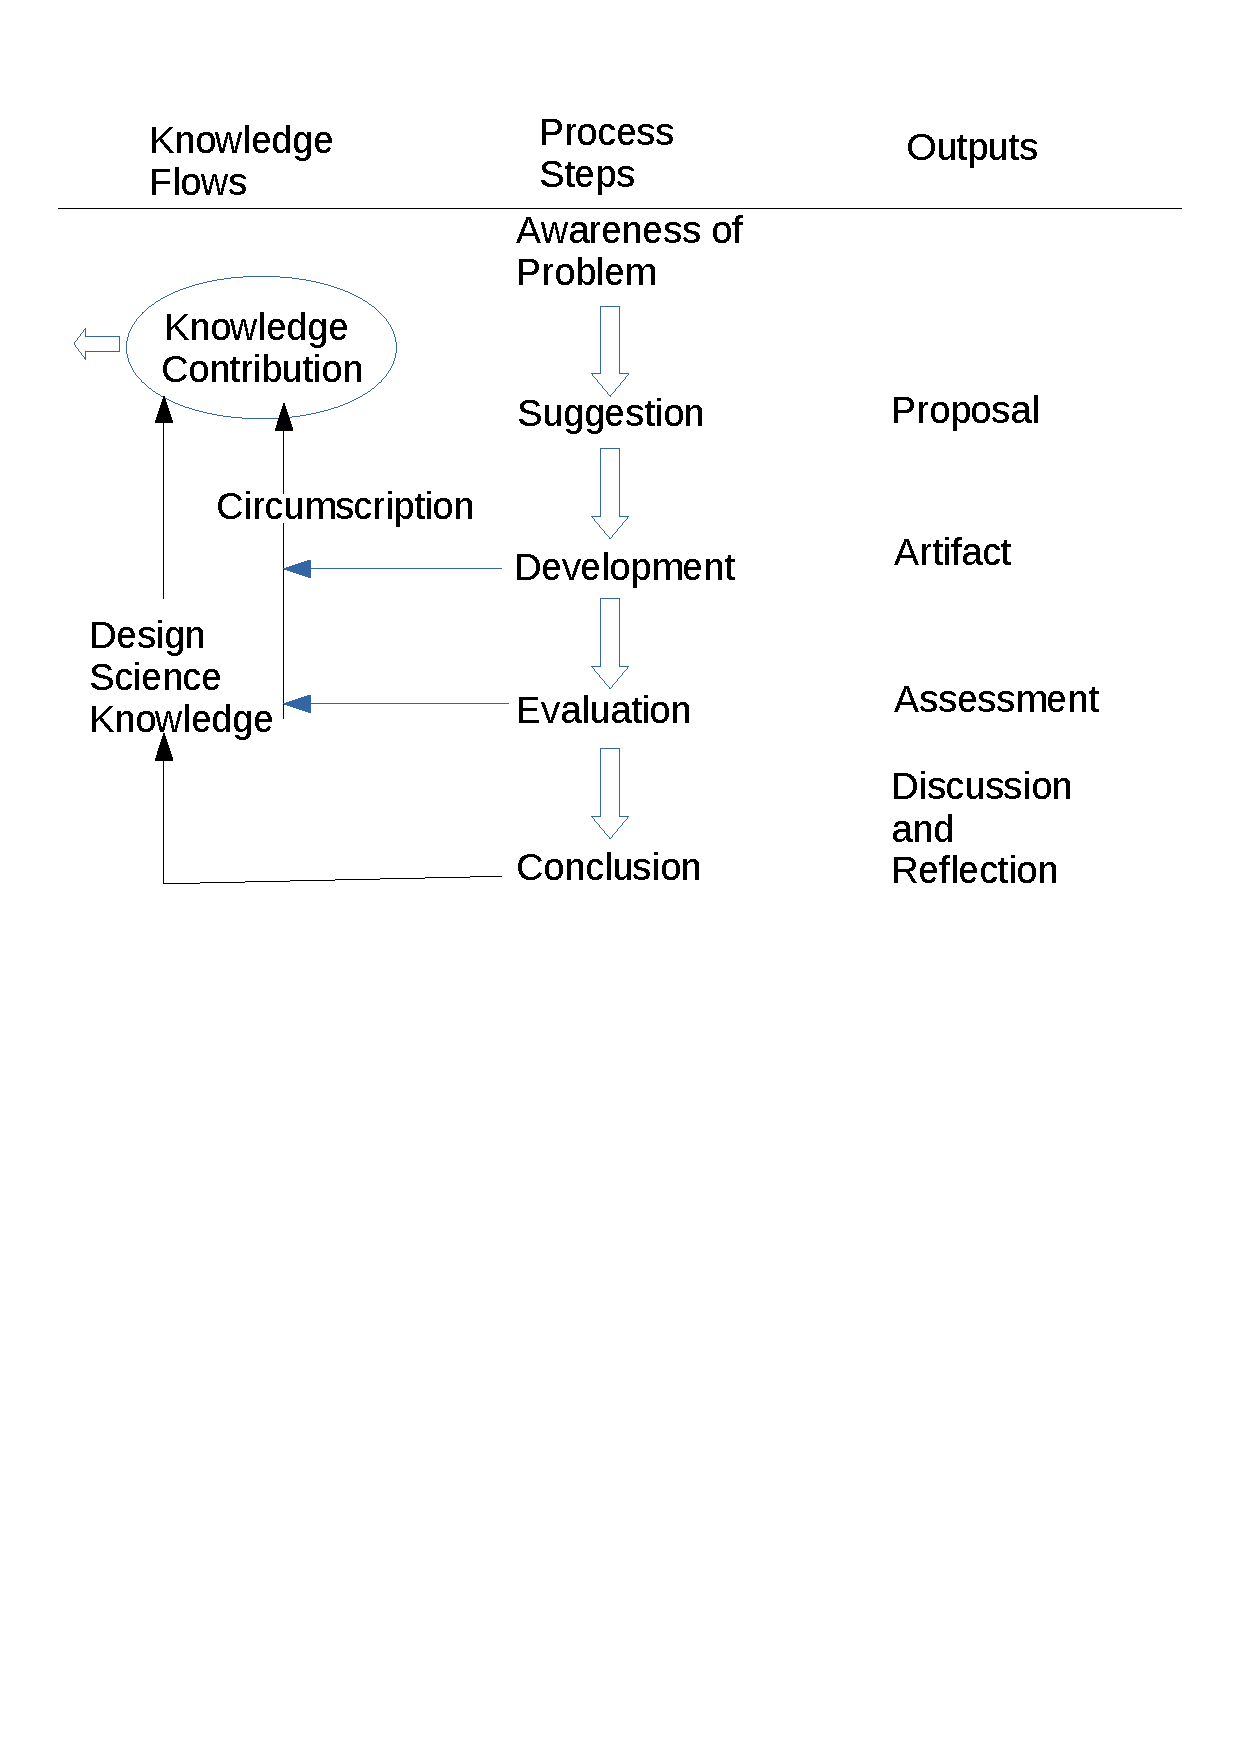
\includegraphics[width=0.9\textwidth]{cropped_dsr.pdf}
\caption{Design Science Research Process Model (DSR cycle)}
\label{dsr}
\end{center}
\end{figure}

\paragraph{Suggestion} The suggestion phase follows after the awareness phase and includes a proposal along with a tentative design of the proposed solution. The tentative design also comprises of the specifications of the planned artifact. This phase, therefore, is a creative step where new solutions can be visualised based on the combination of existing and new solutions. In the case of this thesis, through researching the existing IoT device management systems and blockchain technology, an attempt has been made to implement a proof of concept that can facilitate device management over blockchains.

\paragraph{Development} In this phase, the tentative design proposed in the Suggestion phase is further developed and implemented. During this phase, the proof of concept system is realised based on the suggestions proposed in the previous phase. 

\paragraph{Evaluation} Once the artifact is implemented, it is analysed and evaluated using various criteria as deemed implicit or as defined in the proposal. Evaluation of the artifact can include various methods such as observing, testing or by the way of experimenting. Deviations from the expected results are examined and discussed about in the scientific document. Section \ref{Section: Test Methodologies} under the Evaluation chapter talks in detail about various test methodologies, and the ones considered for this system.

\paragraph{Conclusion} This phase is the supposed end of the research cycle, or the ending point of a particular research effort. The results can then serve as a base for further research or for development of a larger system.
\newpage
\section{Blockchain Technology}

The introduction of Bitcoin \cite{bitcoin} in 2009 introduced a new era in the digital world. It illustrated some novel approaches to computing such as decentralization, where no one server holds control of the network, immutability, where data once written can never be erased, as well as the ability to issue and transfer currency recorded into an open ledger called the Bitcoin blockchain, without any third party. As people started delving more into the blockchain technology underpinning Bitcoin, they realized that the scope of blockchain itself can be extended to a much wider range of applications. Theoretically, the transactions on the blockchain could be used to represent more than money, e.g. complex agreements between two parties. 

A few aspects of these solutions that should not be neglected, are the cost of the services and the fact that too much control is given to the data administrators, or middlemen. That is where blockchain technology is at an advantage. Blockchains are immutable, and serve as ledgers that contain records of every transaction ever made among participants in a given network, encrypted into blocks using a cryptographic hash function SHA256\footnote{SHA256 stands for Secure Hash Algorithm 256-bit}. The technology supports a feature called smart contracts that validate whether terms are met by each party.

Blockchains have been classified into three main types according to the level of access granted to the users participating in the network. \cite{ethereum1} categorizes it into public blockchains, private blockchains and consortium blockchains. Public blockchains are those that can be participated in and read by anyone; Consortium or permissioned blockchains are ones where the miners are chosen in advance and therefore are partly decentralised; and Private blockchains are those that can be read by anyone but written to only by private parties such as organisations. In this thesis, the intention of the larger system is mainly to have a mix of consortium and public blockchains. The smaller proof of concept system this thesis uses however, makes use of a private blockchain to test the system.

The subsequent sections delve into the details of how Blockchain Technology operates and the real world implementations of Blockchains.

\subsection{Architecture}

The network architecture of a Blockchain distributed network is peer-to-peer, and is based on top of the network layer. Peer-to-peer network, also known as P2P, refers to a group of computers acting as a node for sharing files within themselves. The Blockchain, therefore, runs on a distributed network of servers, also known as \textit{nodes}. These nodes in the network serve the purpose of providing a consensus on the state of the blockchain at any given time, and have a copy of the blockchain stored in them. The fundamental application of the Blockchain is a transaction ledger, sort of like a secure public ledger, that stores all the transactions that take place within the network. This makes it a very secure and transparent decentralised system. 

\subsubsection{Network Architecture}


\begin{figure}[H]
\begin{center}
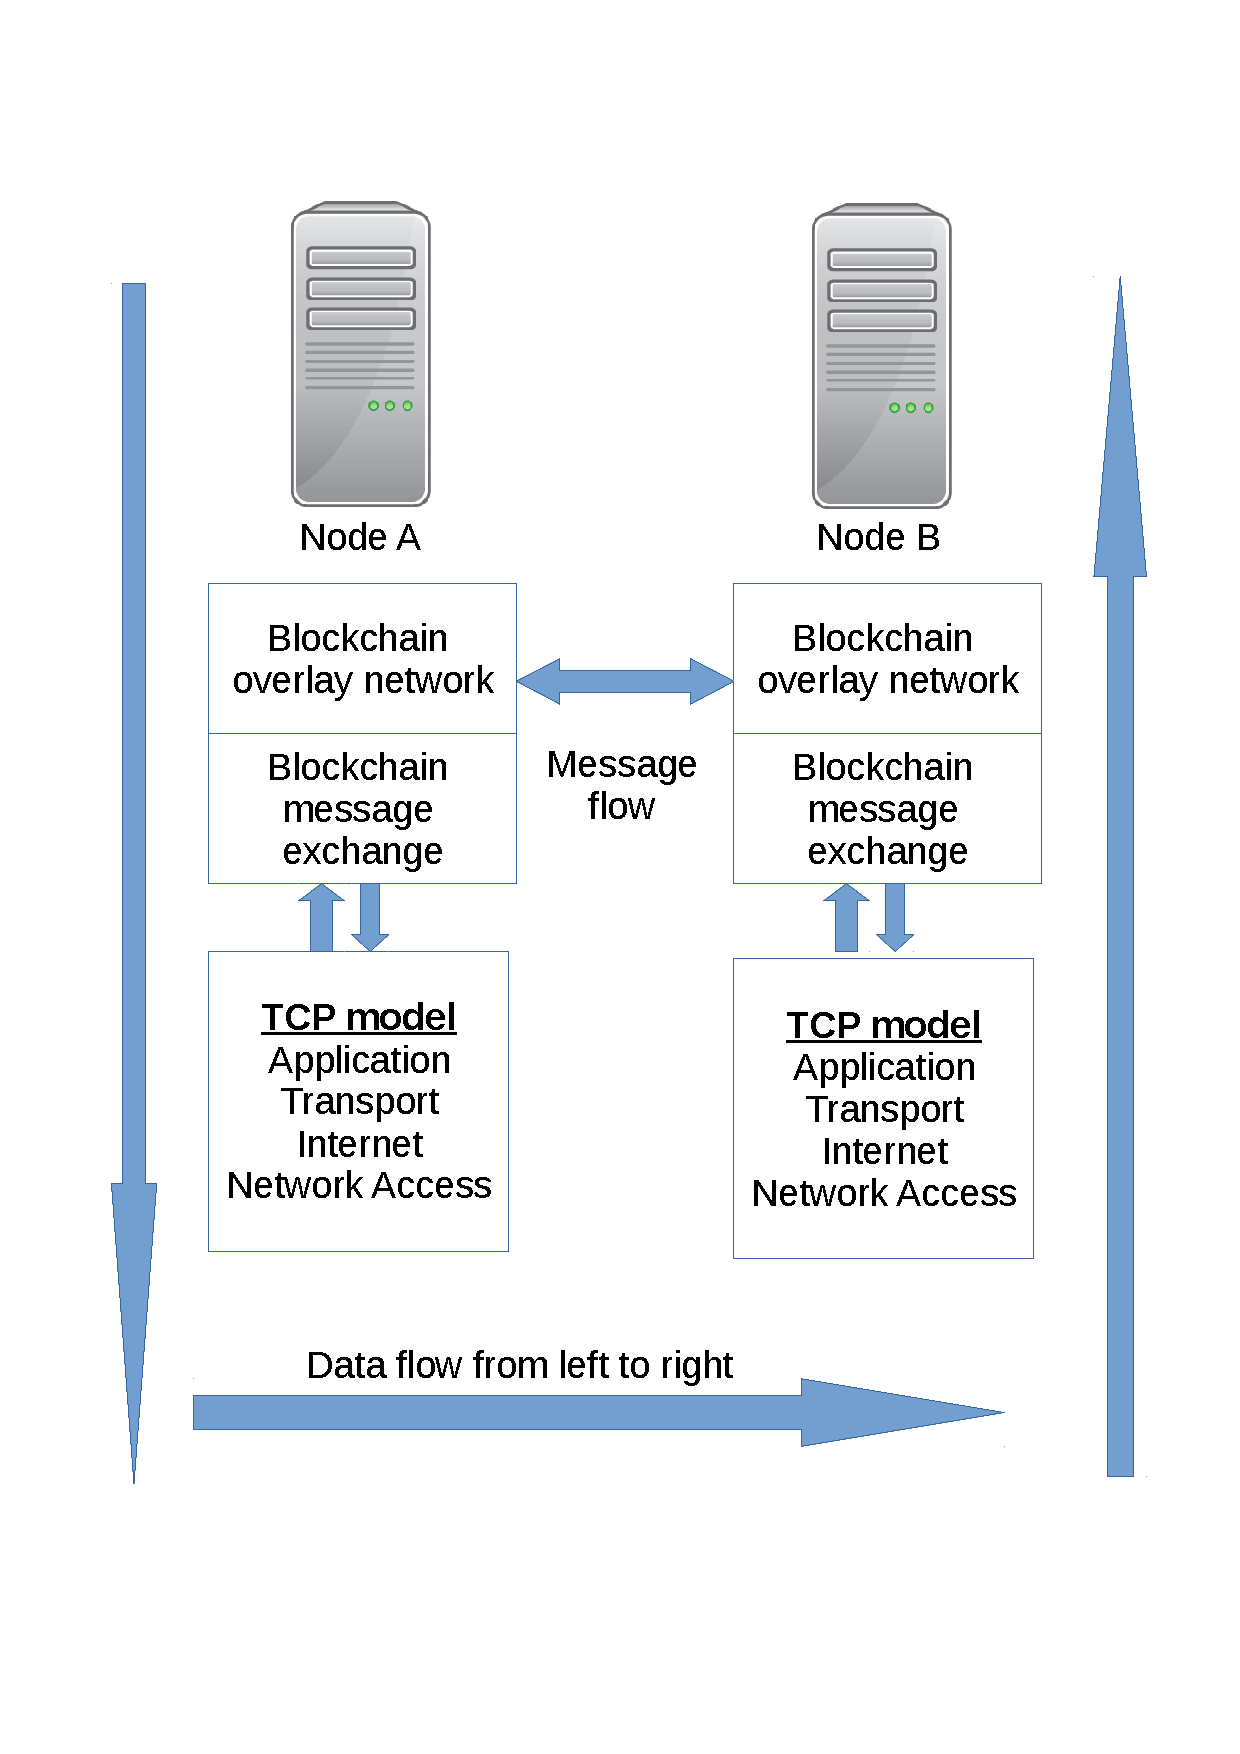
\includegraphics[width=0.6\textwidth]{cropped_BlockchainNetworkStack.pdf}
\caption{Blockchain Network Architecture}
\label{Blockchain Network Architecture}
\end{center}
\end{figure}

\subsubsection{Nodes}
The nodes or clients connected to the network in the Blockchain system are an essential part of the system. They support various functions such as routing, mining, storing the blockchain data and serving as a wallet. All nodes participate in verification and propagation of transactions, and are enabled with features including discovering and maintaining connection with their peers. They also maintain a copy of the ledger, or the blockchain, which contains data about all the transactions that have ever happened, thereby eliminating the need of having a centralised server to store it. 
Nodes can also act as \textbf{Miners}, and help verify and validate all the transactions made by all the users. All miners are nodes, but all nodes are not necessarily miners.

The nodes are mainly of three kinds namely, full nodes, \textbf{simplified payment verification (SPV)} clients and web clients. Web clients, usually called \textit{wallets}, are stored on third party servers and can be accessed through web browsers. SPV nodes usually include clients that do not possess enough hardware capabilities like mobile devices, or more constrained devices like embedded systems. These SPV nodes do not need to store a copy of all the transactions in the blockchain, and instead store only the block headers. These nodes have a slightly different way of verifying transactions from the full nodes, since they do not keep a track of all the transactions taking place on the blockchain. They depend on their peer nodes to provide the transaction information they require, on an on demand basis. Full nodes, on the other hand, are the nodes that store an up to date copy of the blockchain in its entirety. 


Once the nodes are connected to the Blockchain network, they start looking for other peers to connect to, on a particular port over TCP. This process of node discovery is also called as the discovery protocol.
\subsubsection{Transactions}

Transactions are data structures stored in files called blocks. They are not encrypted and are typically linked to previous transactions, thus forming a chain. A digital currency owner digitally signs the previous transaction with their public key and a hash is created out of it. The owner of the previous transaction then signs the hash with their private key. Figure \ref{Transaction ownership chain} illustrates a simplified version of the ownership chain, as explained in \cite{bitcoin}. In more complex cases, the number of inputs and outputs can be multiple. A transaction contains a number of fields as shown in Table 1.\newline
\begin{table}[H]
\centering
\label{table:transaction_fields}
\begin{tabular}{|l|l|l|}
\hline
\textbf{Size}      & \textbf{Field} & \textbf{Description} \\ \hline
4 bytes            & Version        & Specifies which rules this transaction follows \\ \hline
1-9 bytes (VarInt) & Input Counter  & How many inputs are included                   \\ \hline
Variable           & Inputs         & One or more transaction inputs                 \\ \hline
1-9 bytes (VarInt) & Output Counter & How many outputs are included                  \\ \hline
Variable           & Outputs        & One or more transaction outputs                \\ \hline
4 bytes            & Locktime       & A Unix timestamp or block number               \\ \hline
\end{tabular}
\caption{Fields in a transaction}
\end{table}

\begin{figure}[H]
\begin{center}
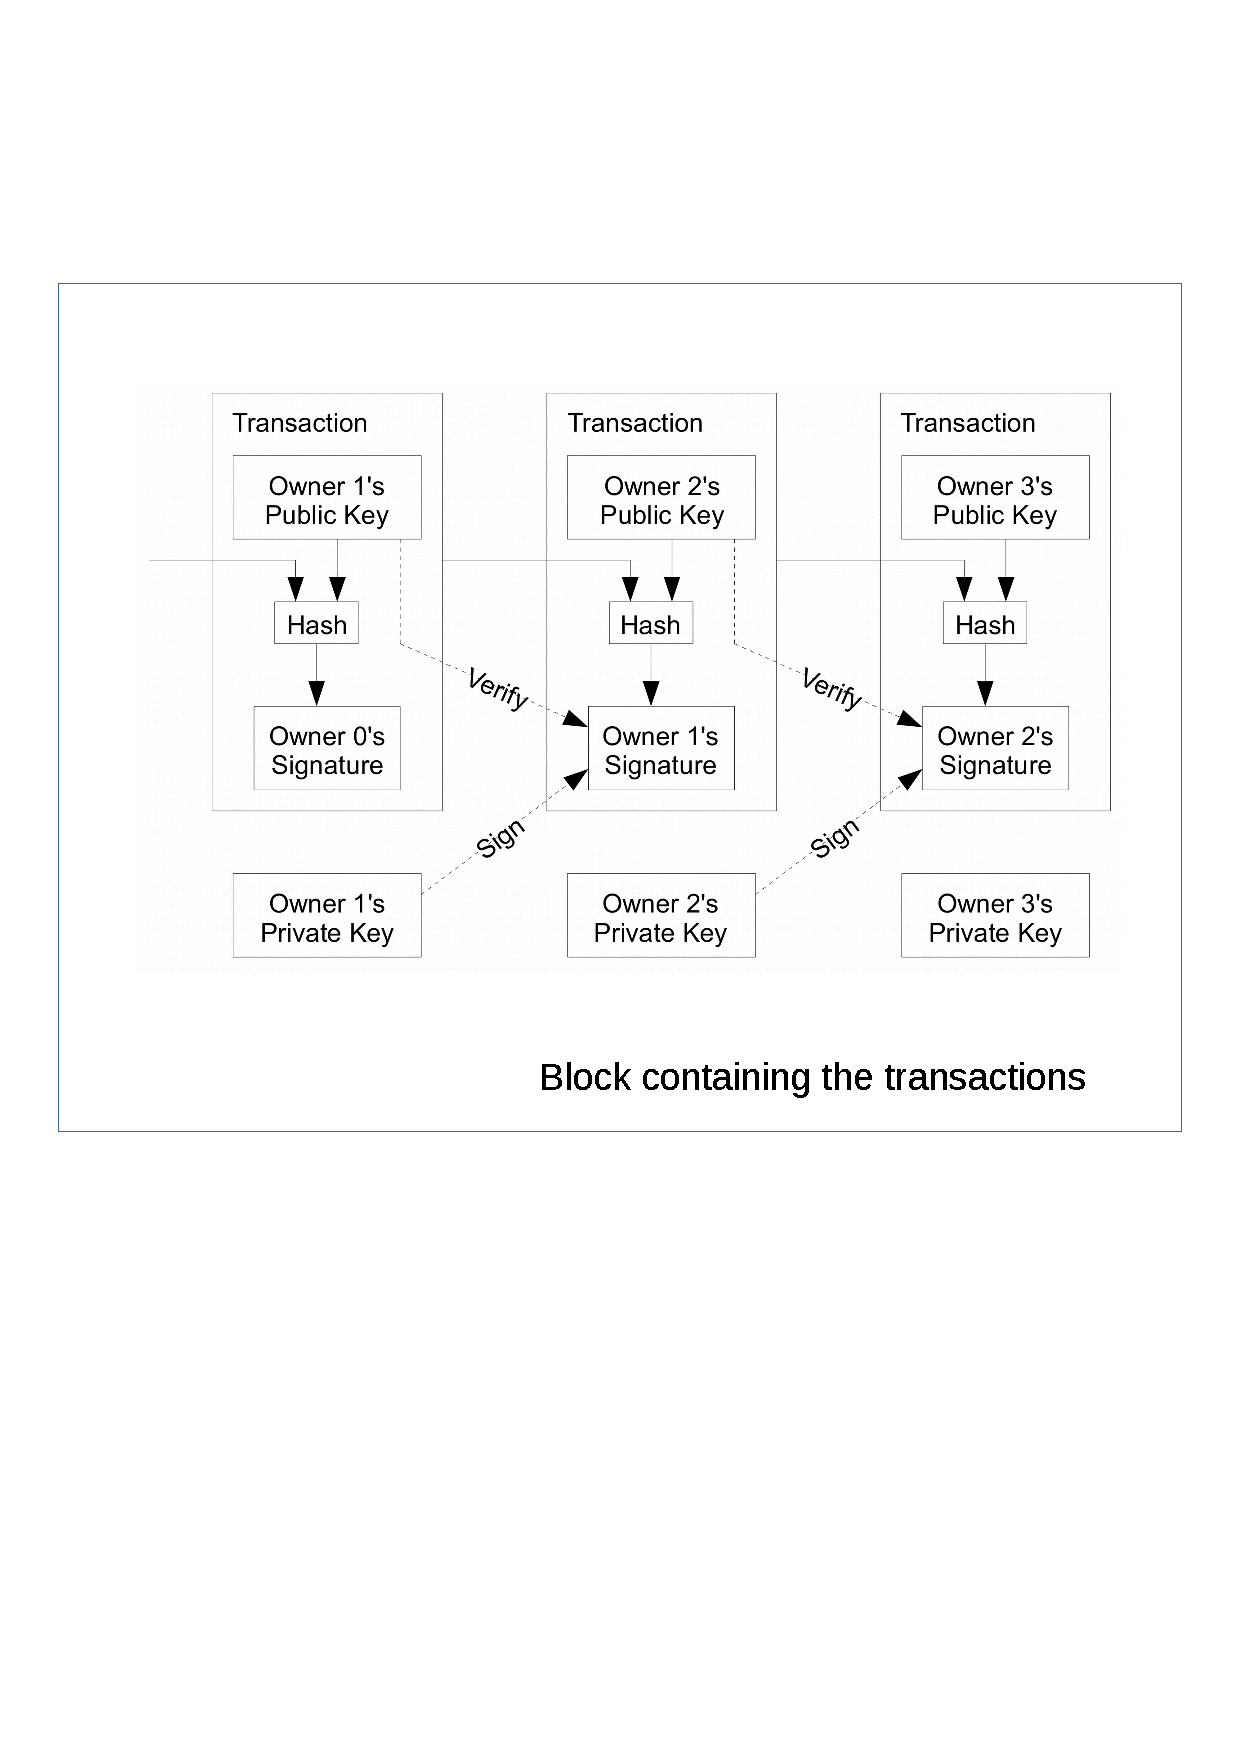
\includegraphics[width=0.7\textwidth]{cropped_Transaction_ownership.pdf}
\caption{Transaction ownership chain}
\label{Transaction ownership chain}
\end{center}
\end{figure}

Most transactions also include a fee that is paid to the miners to keep the blockchain consistent and secure. These miners mine a block which records the transactions on the blockchain and in return receive the transaction cost as an incentive. Most wallets calculate these transaction fees automatically.

\subsubsection{Blocks}


\begin{figure}[H]
\begin{center}
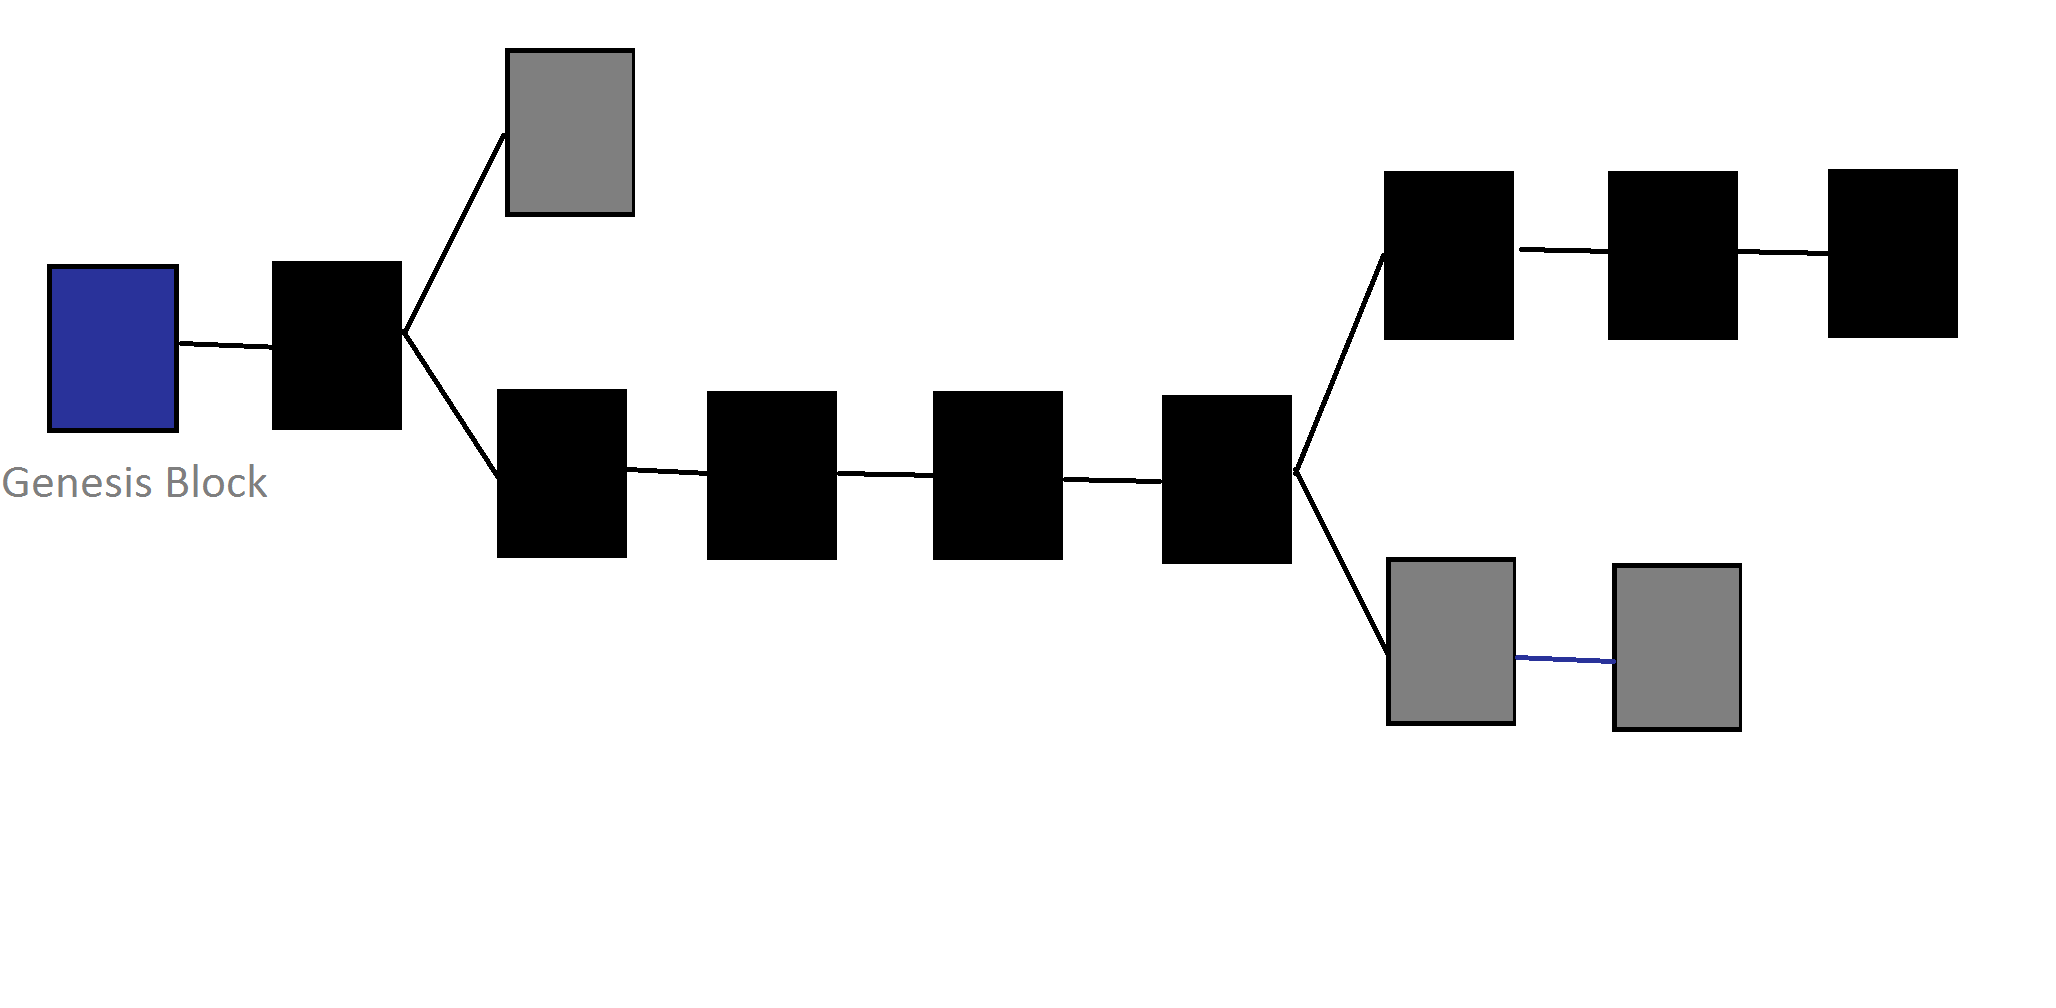
\includegraphics[width=0.7\textwidth]{blockchain.png}
\caption{Blocks in the blockchain}
\label{blocks}
\end{center}
\end{figure}

Figure \ref{blocks} illustrates the linkage of blocks in the Blockchain. The blocks marked in black show the current active blockchain. The ones marked in grey are called stale blocks. A detailed explanation about this has been provided in Section \ref{stale blocks}. The Blockchain is technically an ordered and timestamped linked list of blocks, that provides a record of all the transactions that have ever happened. Each of these blocks is linked to the previous one, i.e. its parent, through a unique hash. These hashes are generated through the SHA256 hashing algorithm. In other words, the header of each block contains a reference to its parent's hash. This linking continues all the way up to the first block in the blockchain, also known as the \textbf{genesis block}. The genesis block is the leftmost blue block indicated in Figure \ref{blocks}. 

A block can have multiple children simultaneously. Each child refers to the same parent block's hash. Ultimately, one of these child blocks becomes the part of the main blockchain. This phenomenon is known as \textbf{forking}. This happens when multiple miners mine and verify different blocks at the exact same time. The blockchain is therefore, called immutable since it is an astronomical expense to recompute the hashes of all the blocks starting from the genesis block. Table \ref{structure-of-a-block} describes the various fields in a block along with their sizes. Table 2 further describes the structure of a block header, explaining the different kinds of metadata associated with the blocks. 
\newline


\begin{table}[h]
\centering
\label{structure-of-a-block}
\begin{tabular}{|l|l|l|}
\hline
\textbf{Size (bytes)} & \textbf{Field}      & \textbf{Description}                          \\ \hline
4                     & Block Size          & The size of the block                         \\ \hline
80                    & Block Header        & Consists of several fields, as shown in Table 3 \\ \hline
1-9                   & Transaction Counter & Number of transactions included in the block  \\ \hline
Variable              & Transactions        & Recorded transactions included in the block   \\ \hline
\end{tabular}
\caption{Structure of a Block}
\end{table}
 
Since the block header is a part of the block, a complete block, including all the transaction information, is much bigger in size than a block header. This is the reason, SPV clients and wallets download just the header files of the blockchain while retrieving their desired block's info from the full nodes connected to the network. 

The \textit{merkle root} field refers to the root of a merkle tree that stores the transaction information in every block. A detailed explanation of Merkle trees is provided at Section 2.1.5.

The \textit{timestamp}, \textit{difficulty} and \textit{nonce} fields are connected to the transaction verification process that the bitcoin miners compete for. \newline

\begin{table}[H]
\centering
\begin{tabular}{|l|l|p{8.2cm}|}
\hline
\textbf{Size(bytes)} & \textbf{Field}      & \textbf{Description}                                                                      \\ \hline
4                     & Version             & Software version                                                                          \\ \hline
32                    & Previous Block Hash & Reference to hash of the previous block                                                   \\ \hline 
32                    & Merkle Root         & Hash of the root of the merkle tree 
containing all the transactions included in the block \\ \hline 

4                     & Timestamp           & Approximate time when the block was created                                               \\ \hline
4                     & Difficulty Target        & Proof of work difficulty for the block                                                    \\ \hline
4                     & Nonce               & Proof of work counter                                                                     \\ \hline
\end{tabular}
\caption{Block Header structure}
\label{block-header}
\end{table}

\cite{ethereum1} explains the validation process of the blocks and decision making process that leads to the addition of a block to the blockchain, using the blockchain paradigm. The process takes place in the following sequence. The system first checks whether the previous block hash that the current block references to, is valid. The time-stamp of the block is then checked, since its value needs to be greater than that of the previous block and less than two hours into the future. The validity of proof-of-work is then checked. If the state of the previous block when compared with the list of transactions returns true, the new block is added on to the blockchain.

\subsubsection*{Block hash and height}
There are two ways to identify a block. First, by its hash. This hash is computed by the peer nodes in the network every time a block is generated. The hash could be stored in a database included in the block's metadata for faster indexing and retrieval of the blocks from the disk. The second way to identify a block would be by its height. The genesis block is at height 0. This method of identification is not absolute because two or more blocks in the blockchain can have the same block height, and it is also possible that two blocks of the same height have the same parent.

\subsubsection{Merkle Trees}

Each block in the blockchain contains a \textit{Merkle tree}, that stores the transaction information. Merkle tree \cite{bitcoinbook}, or a hash tree, is a data structure that helps with verification and summarizing of large sets of data. They efficiently store all the transactions in the block, and their root contains a hash of all the transactions in the block. The merkle trees facilitate the SPV nodes to download just the block headers and still be able to identify whether a transaction is included in a particular block, by obtaining the small merkle path from a full peer node. Figure \ref{merkle-tree} illustrates how merkle trees are used in transactions in a block on the blockchain.

\begin{figure}[H]
\begin{center}
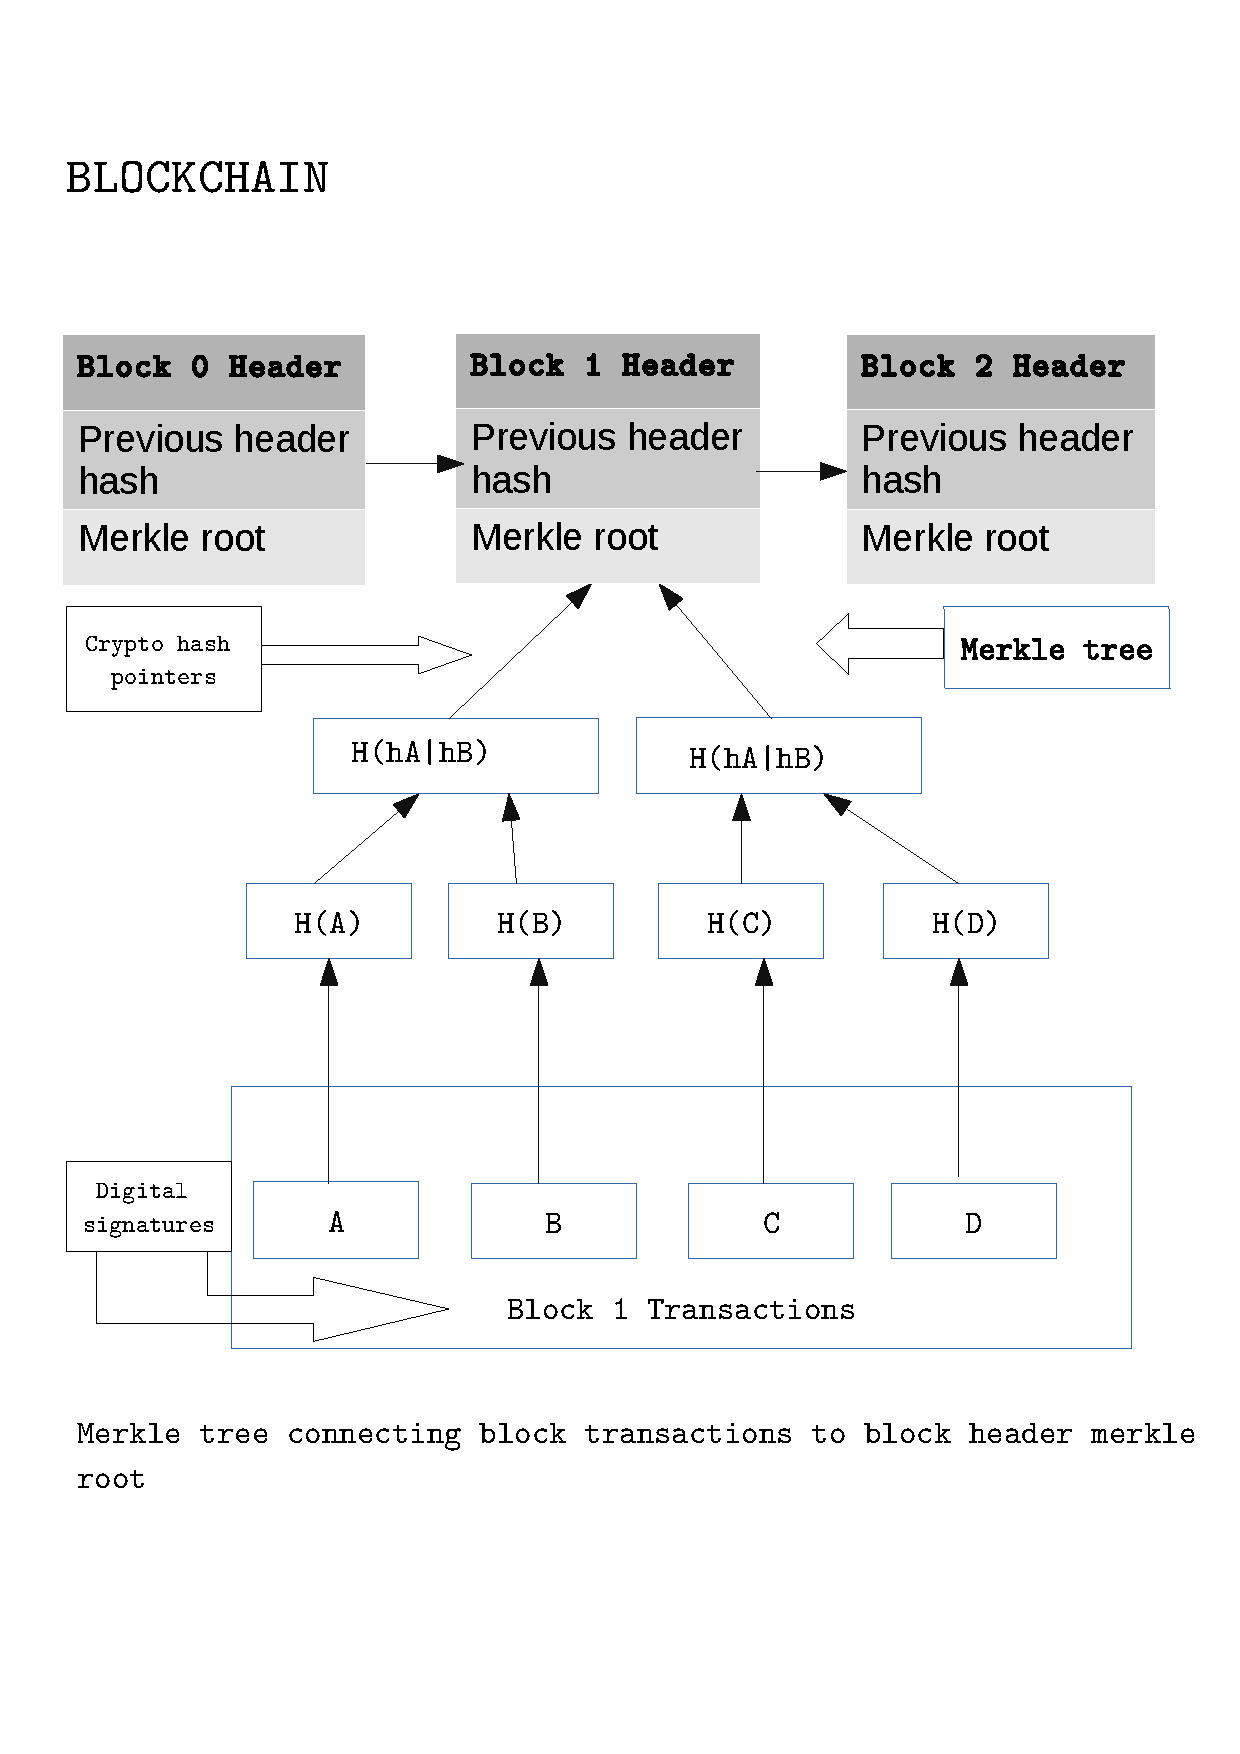
\includegraphics[width=0.8\textwidth]{dgm_blockchain.pdf}
\caption{Merkle Trees in blockchain}
\label{merkle-tree}
\end{center}
\end{figure}

Simply put, merkle trees are used to connect transactions to blocks in the case of Blockchains. Every block header contains a single hash, i.e. the merkle root, which in turn is the root of a merkle tree that contains all the transaction id hashes. It has several layers of checksum that could, therefore, be used to validate individual transactions or even verify a block. Since every merkle root contains a hash of all the transactions in the block, it is not necessary to have a copy of the entire tree. This also helps with pruning the blockchains, as we will discuss later in the \textit{Discussion} section.

\subsubsection{Mining}

There are two major benefits of mining for the blockchain network namely, validation and verification of transactions. Mining also generates new digital currency coins to the network, since these newly minted coins serve as the reward to the miner who solves the next block in the blockchain. 

The first step to mining is calculating the \textit{difficulty level} of the blockchain. All the full nodes connected to the blockchain network recalculate this difficulty level after certain intervals. The level can either increase or decrease based on how long it takes to generate the certain interval of blocks. In the case of Bitcoins, which was the first implementation of blockchains, the interval is 2016 blocks. Thus, the full nodes have to rehash the difficulty level after every 2016 blocks, which leads to an average consensus time of 10 minutes. As the number of miners increase, the rate of block creation also increases. This is turn, leads to an increase in the difficulty level, since it pushes the rate of block creation down to the original time of 10 minutes, in the case of Bitcoin.

The miner then downloads all the transaction and block information that happened previously, and constructs a merkle tree out of them, eventually generating a merkle root. 

In order for it to form a block, a miner is free to choose the number of transactions they want. The only limiting factor to that is the \textit{maximum block size}. As an example, in case of Bitcoins, the maximum block size is 1 MB, and so, depending on the transaction size, a maximum number of transactions that occupy upto 1 MB space can be accommodated in the block. In Ethereum, the maximum block size is not in terms of the storage space it occupies, but rather in terms of the maximum gas limit that it can allow. The role of gas and how it is calculated has been discussed at length in Section \ref{subsection: gas}. A detailed account of how mining takes place in the Ethereum system is mentioned in Section \ref{Section:Ethereum_Mining}.

The miner then generates the block's hash from the block header values and then compares the hash to the current difficulty level of the network. This hash is generated using one of the few consensus algorithms used in blockchain systems, which we delve into, in Section 2.2.

The pseudo code below, where H(n) and H(b) refer to the difficulty level of the new block and the existing block difficulty level respectively, shows the conditions that a block must satisfy in order to be accepted.\newline

\begin{verbatim}
If (H(n) > H(b)) && (Block accepted by the network)
    Block is propagated and miner gets rewarded
else
    Block is rejected
\end{verbatim}

There can also be a possibility of two or more miners generating a block at the same time. This leads to the formation of \textit{Stale} and \textit{Orphan Blocks}. Different implementations of blockchains deal with these stale and orphaned blocks differently, as will be discussed in the blockchain implementation section.

\subsubsection*{Solo and Pool Mining}

There are two ways mining can be done on a blockchain network. The first being, \textit{solo mining} and the second, \textit{pool mining}. As the name indicates, solo mining refers to a single miner trying to generate blocks on the blockchain in exchange for rewards. But owing to the increasing difficulty of generating blocks, and maintaining the mining hardware costs, it is becoming increasingly difficult to mine alone. In case of pool mining, the group needs to have an agreement on reward and risk distribution for each miner. Every pool operates on their own set of rules, sometimes involving extra "fees" for the pool operator. 

\subsubsection{Database}
The nodes connected to the blockchain network need to store a copy of the blockchain. A core client natively uses Google LEVELDB\footnote{LEVELDB: A fast, lightweight database. More information at http://leveldb.org/} database to store the metadata associated with the blocks in the blockchain, which can be stored as per user preferences, such as in a relational database system or even as an unstructured flat file.

\subsection{Consensus Mechanisms}

Consensus is a fundamental problem in Distributed Systems that requires two or more agents to mutually agree on a given value needed for computational purposes. Some of these agents may be unreliable, and therefore the consensus process needs to be reliant. Thus, the need of consensus mechanisms is to facilitate secure updation of a process or a state, in accordance with certain state transition rules, where a distributed set has the right to perform the state transitions \cite{eth-whitepaper}.

The most commonly used consensus mechanisms in case of Blockchains are discussed in this section.

\subsubsection{Proof of Work} \label{Section:PoW}

There are two kinds of rewards a miner can receive for mining a block. First being, the transaction fees from all the transactions picked by the miner for the block formation, and second, the new digital currency created with every block. To be able to earn these rewards, the miners compete to solve a mathematical problem called \textit{proof of work or PoW}. PoW is a consensus algorithm, and is really a brute force crack on a SHA256 hash algorithm. This works as a proof that the miner has used some heavy duty computing resources. The exact condition is that the double hash of every block must be less than the difficulty target\cite{eth-whitepaper}.

\subsubsection*{51\% attack}
Besides the fact that proof of work algorithm consumes a lot of energy, there is another flaw to it called the \textit{51\% attack}. If a single entity were to contribute to more than 51\% of the bitcoin network's mining, they would be able to fully control the network and modify the ledger according to their needs. While this attack is theoretically possible, it would cost the miners an enormous amount of money as well as computational power. 

\subsubsection{Proof of Stake}

As discussed earlier, PoW algorithm estimates how much of the network agrees on the blockchain's existing state at that point, using the difficulty and nonce fields. This requires a lot of computational resources, which in turn requires a lot of expenditures on the part of the miner. This is the main reason miners are compensated with adequate digital currency, which are created whenever a block is mined and added to the blockchain. Therefore, motivated by the problem of energy efficiency and usage of a huge amount of computational resources, a consensus algorithm called Proof of Stake was suggested. 

In case of the proof of stake (PoS) algorithm, the consensus is achieved on how much of the cryptocurrency agrees with the present state of the blockchain. PoS therefore, requires the cryptocurrency owners to prove that they own a certain amount of cryptocurrency which equates to their \textit{stake} in the currency \cite{pos}. The required amount of coins (also known as the target) to be able to be a part of the proof of stake network is usually set in advance by the network using a difficulty adjustment process similar to that of proof of work.

\subsubsection{Proof of Burn}

Proof of burn\cite{proofofburn} is an alternative distributed consensus algorithm to PoW and PoS. The idea is to destroy or \textit{burn} some coins by sending them to an unverifiable address on the blockchain network. This helps reduce the total supply of currency on the blockchain and increase the value of the coins in circulation. Destroying some of their currency would ensure that the miners get lifetime rights to mine, since in this case the chances of being allowed to mine is a lottery among the owners of destroyed coins. Therefore, the more burnt coins, higher are the chances of the miner to win in the lottery. Different implementations of proof of burn handle the lottery system differently. One such system that implements proof of burn in their cryptocurrency system, is called Counterparty \footnote{Counterparty: For more information - http://counterparty.io}.

\subsubsection{Delegated Proof of Stake}
Delegated proof of stake(DPoS)\cite{dpos} tries to combine proof of work and proof of stake characteristics and uses a decentralized voting system. The distinguishing factor in DPoS is that the top 101 delegates are the ones securing and forging the network. These delegates are determined by their stake in the network just as in proof of stake.

\subsection{Double Spending}

One question that arises from the use of digital currency is that of double spending \cite{bitcoin} i.e., currency counterfeit. Can the cryptocurrency owner be sure nobody else is falsely claiming ownership to their coins? How would one know if the amount the sender send, actually goes into the blockchain? Physical currency notes solve the problem easily because the same note cannot be given to two different people at the same time. For a virtual currency, the main issue seems to be that of synchronisation. In case of Bitcoins, if a user attempts to spend the same bitcoin twice for example, the miners reject both the transactions to prevent the same bitcoins from going two separate ways. However, if the user does succeed in double spending, one of the receiving parties does not receive any bitcoins. In this case, the accepted transactions is included in the blockchain and is irreversible. Therefore, in effect, Blockchains eliminate the issue of double spending.

\newpage
\section{Blockchain Implementations}
This chapter talks discusses about various Blockchain implementations, with more focus on the Bitcoins and Ethereum systems. The chapter is organized as follows. Section 3.1 explains the Bitcoins system, Section 3.2 explains the Ethereum system and Section 3.3 talks about some other well known Blockchain implemetations. Table \ref{blockchain_implementations} gives an overview of the various blockchain systems discussed in this chapter and their salient features. 

\subsection{Bitcoin}

Bitcoin is a cryptographic currency (also known as a cryptocurrency), that serves as a digital financial asset, and was created by programmer(s) under the pseudonym of Satoshi Nakamoto. The main idea behind proposing Bitcoins was not to rely in the trust of centralised banks, since they invest people's money in the market with very little in reserve\cite{bitcoin}. Therefore, Bitcoin focuses on providing total transparency. Every time a bitcoin owner makes a payment, the transaction is broadcast over the network and recorded in the blockchain forever, thereby making it an immutable transaction.

Bitcoin uses public key cryptography, peer to peer networking and proof of work to make transactions and verify them. 

\subsubsection{The Bitcoin Network}

Bitcoin uses public key cryptography, peer to peer networking and proof of work to make transactions and verify them. It was the first blockchain to be conceptualised and implemented.

The Bitcoin system is programmed such that a new block is created once every 10 minutes. Even if a block were to get created in under the stipulated time of ten minutes, albeit with a very small chance since it is very computationally expensive to be able to do so, it can only  happen for a very short time. The difficulty adjusts itself until the block creation time becomes ten minutes again, which is usually after every 2016 blocks in case of Bitcoins. The 10 minute block creation time, as described in \cite{bitcoin}, was chosen as a compromise between propagation time of new blocks in large networks and the amount of work wasted due to chain splits. A faster block creation time would mean that there could be more chances of many miners mining a block at the same time, and that would lead to more forks. If a fork is not a part of the \textit{longest} chain, it becomes an orphan block. We discuss more about orphan blocks in Section 3.1.3. The choice of ten minutes also takes into account, the slow network speeds in many parts of the world.

\subsubsection{Transactions and Scripting language}

An interesting fact to note is that there are no balances in bitcoin, or rather there are unspent transaction outputs (UTXO) in the blockchain. Whenever some bitcoins are received, they are recorded as UTXO. The receiver then scans the blockchain and adds up all the UTXO associated with their account, and figures out how many they own. Thus, sending someone a bitcoin actually means creating a UTXO corresponding to the receiver's address, which they can spend. An output typically consists of two fields namely, the amount and a locking script. A \textit{satoshi} is the smallest denomination of the amount that can be sent. The locking script sets out conditions that need to be fulfilled in order to spend the UTXO.

The Bitcoin nodes follow a scripting system to validate transactions. It follows a scripting language called \textit{Script}. When a transaction is validated, an unlocking script runs simultaneously with the UTXO's locking script to verify whether the condition that facilitates spending is satisfied. There are five standard transaction scripts including pay to public key hash, multi signature, pay to script hash, public key and OP\textunderscore RETURN. OP\textunderscore RETURN is the only transaction output that allows any data not related to the transaction itself. This data cannot be spent, and can be of 40 bytes. Needless to say, it does not form a part of the unspent UTXO calculations for account balance.

\subsubsection{Stale and Orphaned Blocks} \label{stale blocks}

Often during mining, there are many blocks that do not end up becoming a part of the blockchain. There can be several reasons causing this phenomenon. \textit{Stale blocks} are those that have a preceding block, but are not a part of the main blockchain. One possibility of a block turning out to be stale is when two miners produce valid blocks simultaneously and one of them is propagated into the network slower than the other one. The slower block ends up being discarded, and the more widely accepted block becomes a part of the blockchain. This is more common when the difficulty is low, which lets many miners solve the proof of work algorithm in a short time frame. Such situations result in a conflict, and usually the computationally \textbf{longest} chain wins. The \textbf{length} of a chain, in this case, is measured by the amount of work it took to find an individual block in the chain. Figure \ref{longest_chain} illustrates this with an example. In this case, when block B3 is mined, the second chain, i.e. chain B is chosen because it is longer.\newline

\begin{figure}[H]
\begin{center}
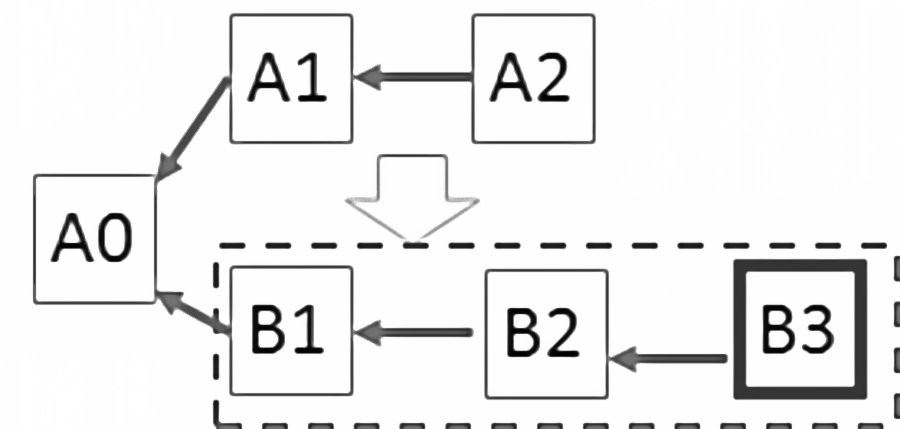
\includegraphics[width=0.5\textwidth]{longest_chain_bitcoin.jpg}
\caption{Longest chain selection in Bitcoins}
\label{longest_chain}
\end{center}
\end{figure}

Orphaned blocks, on the other hand are those blocks that do not have a valid parent. When a miner downloads an orphaned block, they first have to find and validate the unknown/missing parent block, and then proceed to validate the former orphaned block. 

As many miners compete to generate blocks on the blockchain, the possibility of having stale or orphaned blocks is quite high. The full nodes in the blockchain network, keep such blocks in the memory, while trying to validate the ancestry of the orphaned blocks. These blocks are evetually discarded and the rewards or the transaction fees associated with these blocks become \textit{unspendable}. This phenomenon of generation of orphaned blocks is also known as \textbf{Chain Reorganization}. The latest version of the Bitcoin system, at the time of writing this thesis, does not generate any orphan blocks anymore due to a recent change in their download mechanism\footnote{Change in Bitcoin 1.0: http://bitcoin.stackexchange.com/questions/5859/what-are-orphaned-and-stale-blocks}.



\subsection{Ethereum}

Ethereum was designed by a Bitcoin developer named Vitalik Buterin in 2013, who wanted to build a platform to facilitate development of decentralised applications, also known as \textit{DApps}, on top of the blockchain. Ethereum has its own cryptocurrency called \textit{ether}, and an internal currency to pay for computations and transaction fees called \textit{gas}. The decentralised applications can be programmed with a built in Turing complete language called \textit{Solidity} \cite{eth-whitepaper}. A turing complete language refers to a programming language that can solve any computational problem if enough time and space are provided. Ethereum uses PoW as its consensus mechanism, but is soon switching to PoS.

\subsubsection{Ethereum Accounts}

In Ethereum, an account is an object with a unique 20 byte address together with state transitions. Transitions refer to the data and value transferred between two accounts. There are two  kinds of accounts namely, \textbf{externally owned accounts (EOA)}, that work with private keys and \textbf{contract accounts}, that are generated when a contract code is uploaded into the blockchain. EOAs do not contain any code, and are meant for signing transactions to produce messages from these accounts. Contract accounts act on those messages which usually result in activating the contract code that these accounts contain. A contract is basically a software application that exists in the execution environment and is triggered whenever a message triggers its code. A contract account has its own contract memory that allows the persistent variables of the contract to be stored. 

An account contains the following information. A transaction counter, that ensures a particular transaction takes place only once, balance of the account, contract code if any, and its own memory which usually houses contract specific data structures and the values stored in them. Ethereum uses Merkle trees to keep a track of all the EOAs and contract accounts.

\subsubsection*{Difference between Transactions and Messages}

\cite{eth-whitepaper} says that a transaction in Ethereum is a signed data package that contains a message to be sent from an EOA. Transactions contain the fields as described below:
\begin{itemize}
\item Transaction receiver 
\item Sending EOA's signature
\item Value of ether to be transferred 
\item Data field
\item STARTGAS value, the maximum number of possible computational steps in the transaction execution
\item GASPRICE value, fees paid by the sending EOA for every computational step
\end{itemize}

The last two fields have been introduced in Ethereum transactions to prevent denial of service attacks. The reason they decided to set a limit on the number of computational steps for a transaction, was to avoid accidental infinite loops or resource wastage in the code. As discussed earlier, the unit used to measure fees per computation is called \textit{gas}. Certain operations that involve more computations or require storing information as a part of the state involve more gas expenditure. This way the attacker will need to pay an appropriate amount of gas for every resource they utilize. 

Messages and transactions are almost identical, except for the fact that messages are produced by contract accounts, and that these messages exist only within the execution environment. The fields that a message is comprised of are:

\begin{itemize}
\item Message sender (contract account)
\item Message receiver
\item Value of ether if needed
\item Data field
\item STARTGAS value
\end{itemize}

\subsubsection{GHOST protocol}

\begin{figure}[H]
\begin{center}
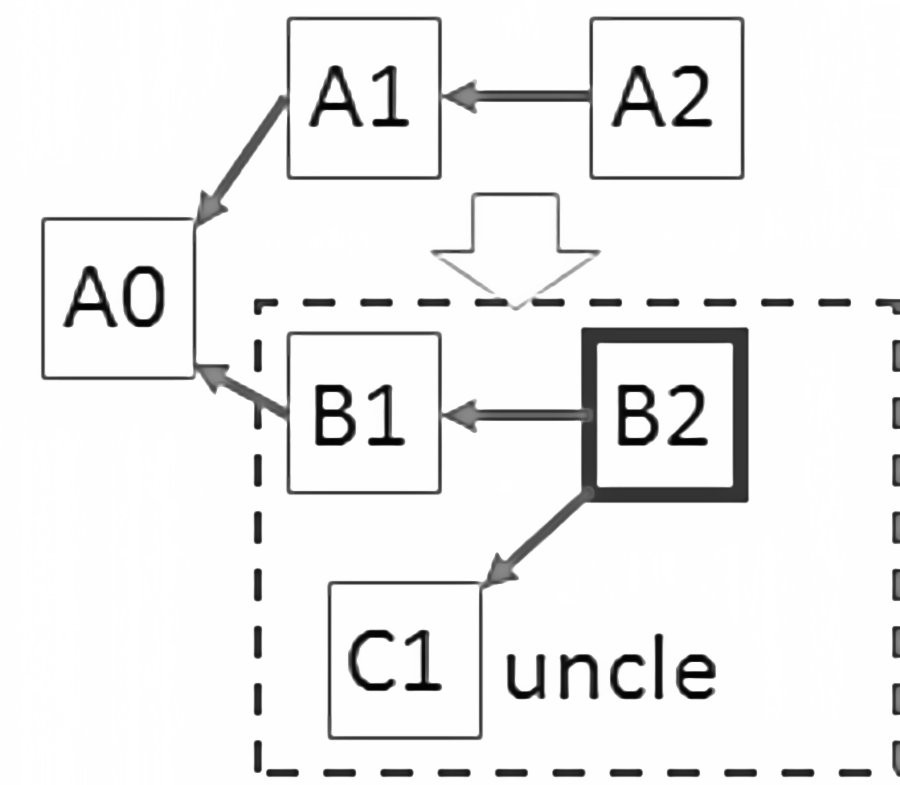
\includegraphics[width=0.5\textwidth]{uncle_ethereum.jpg}
\caption{Ethereum GHOST protocol}
\label{ghost}
\end{center}
\end{figure}

The main idea of Greedy Heaviest Observed Subtree or GHOST \cite{eth-whitepaper} was to \textbf{securely} cut down the consensus time for the bitcoin blockchain. This protocol tries to solve two problems. First, the problem concerning reduced security of the blockchain. The current process involves a high possibility of having stale blocks, and having a faster confirmation time would increase the stale rate much more. To deal with this issue, the calculation must involve taking the stale blocks into account when trying to calculate the \textbf{heaviest} chain. This means that the calculation of the chain into which maximum amount of total work was done, includes the stale descendants of the block's parent. Due to this, it is possible to increase the rate of transaction without compromising the security of the blockchain. In Ethereum, the stale blocks are referred to as \textit{Uncles}.

Ethereum implement GHOST in a simplified way, wherein it goes only seven generations down. The way it has been defined in the Ethereum code is as follows.

\begin{enumerate}
\item A block should specify atleast one Parent and zero or more Uncles.
\item An Uncle of block A must have the following characteristics:
\begin{itemize}
\item Should be different from all uncles included in previous blocks and all other uncles included in the same block.
\item Cannot be an ancestor of block A.
\item Should be a valid block header
\item Should be a direct child of the k\textsuperscript{th} generation ancestor of A, where \begin{verbatim}
2 <= k <= 7.
\end{verbatim} 
\end{itemize}
\item For every uncle U in block A, the miner of A gets an additional 3.125\%, and the miner of U gets 93.75\% of the standard mining reward.
\end{enumerate}

According to \cite{eth-whitepaper}, Ethereum implements a limited version of the GHOST protocol due to two reasons. Firstly, an unlimited version would be too complex with all the calculations involving which Uncle block is valid. Secondly, the unlimited version of GHOST would make the miners greedy to mine the Uncle blocks, thereby making them vulnerable to mining on possibly the chain of a public attacker.

By incentivising uncle mining, the Ethereum system acknowledges the energy spent on the generation of stale blocks. 

\subsubsection{Smart Property and Smart Contracts} \label{Section:Smart_Contracts}

Smart contract \cite{NICK} is a theoretical concept developed in 1994 by Nick Szabo to create self-enforcing and perpetual computer software aimed at replacing legal contracts. According to his description, 

"\textit{A smart contract is a computerized transaction protocol that executes the terms of a contract. The general objectives are to satisfy common contractual conditions (such as payment terms, liens, confidentiality, and even enforcement), minimize exceptions both malicious and accidental, and minimize the need for trusted intermediaries. Related economic goals include lowering fraud loss, arbitrations and enforcement costs, and other transaction costs.}"

In effect, it means that a smart contract is a distributed contract that can serve as an agreement between people and the blockchain without the requirement that both parties trust each other. 

Smart Property\cite{NICK}, is property controlled using smart contracts. This property could be a physical things such as a house or a box, or a non physical entity such as market shares or even permissions to a file server. The main function of a smart property is that it can be dealt with in a trustless way.  

In case of Ethereum, smart contracts are objects that have their own Ethereum accounts. These objects contain programs that can store data, make decisions, communicate with other contracts via messages, or even send money to other accounts. These contracts are established in the blockchain by their owners, but their execution is taken care of by the Ethereum network. They exist in the blockchain forever. Contracts are programmed in a turing complete language called \textit{Solidity}. It can be thought of as a database slot that one can query or alter by passing messages to the contract to access its functions managing that database. 

\subsubsection*{Smart contract code execution}

By definition, a contract is a written or a spoken agreement between two or more parties. But in the case of Ethereum, a smart contract is more like an application containing instructions for itself, that is activated every time a transaction is made to its corresponding Ethereum account. These instructions are written in a scripting language supported by the cryptocurrency system which lets the smart contract access desired transaction, message or other pertaining information on the blockchain. The scripting language in the case of Ethereum is a high level Turing complete, stack based and object oriented language that is executable on the Ethereum Virtual Machine (EVM). The EVM initially supported two languages namely, Solidity and Serpent. But Serpent is not officially supported anymore. Solidity is influenced by Javascript, C++ and Go languages, whereas Serpent is built to be very similar to the Python programming language. 

During the block validation process, each miner tries to verify the portion of the smart contract code responsible for the transactions with respect to the current block\cite{eth-whitepaper}. Figure \ref{smart contract deploy} shows how a smart contract resides in the blockchain network.

\begin{figure}[H]
\begin{center}
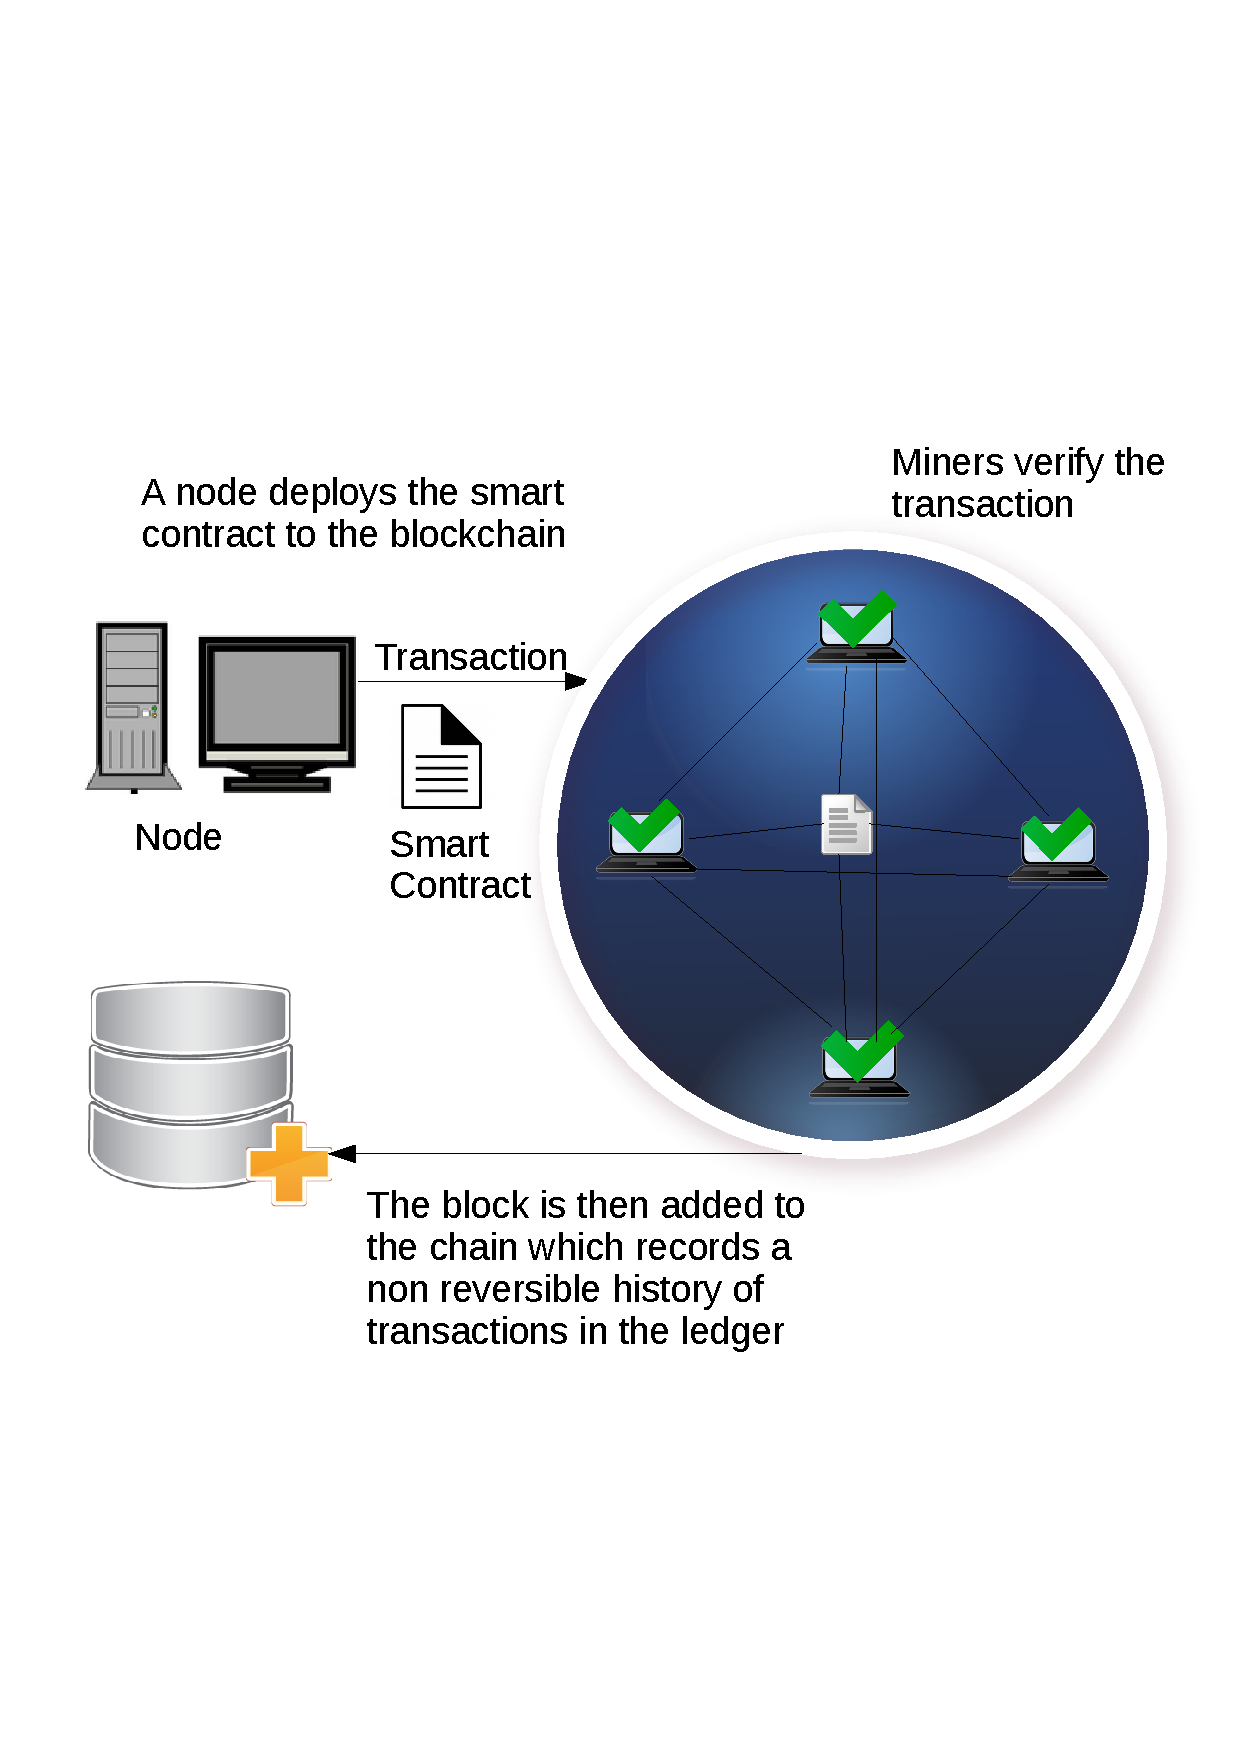
\includegraphics[width=0.8\textwidth]{cropped_smart_contract.pdf}
\caption{Simplified view: Deployment of smart contracts in the blockchain}
\label{smart contract deploy}
\end{center}
\end{figure}


\subsubsection*{Gas} \label{subsection: gas}
It is the coded logic in the smart contract that enables transfer of currency or data from one place to another, through \textit{conditional transactions}. These conditional transactions in the blockchain require a certain amount of computational effort, depending on the type of operation, owing to the fact that the miner nodes in the network are the ones responsible for computing the logic and altering the state of the blockchain. In the Ethereum blockchain, the computational costs are determined by the unit called Gas\textsubscript{price} or \textit{gas price}. Gas\textsubscript{price} is usually set by the developer, and if it is set within certain bounds, the transaction corresponding to that gas price may be accepted by the miners. 
Each operation requires a fixed amount of gas e.g., 3 units of gas for an ADD operation or 5 units of gas for a multiplication (MUL) operation. Table shows an example of some important operations along with the proportional gas units they consume.

\begin{table}[H]
\centering
\label{gas}
\begin{tabular}{|l|l|}
\hline
\textbf{Operation} & \textbf{Gas units} \\ \hline
PUSH               & 3                           \\ \hline
ADD                & 3                           \\ \hline
MUL                & 5                           \\ \hline
SUB                & 3                           \\ \hline
OR                 & 3                           \\ \hline
AND                & 3                           \\ \hline
\end{tabular}
\caption{Gas consumption for some operations}
\end{table}

Every transaction needs to be supplied with enough gas, also known as \textit{startGas}, to support the computation costs and its storage. The residual gas is then given back to the user who initiated the transaction. The wallets usually calculate the amount of startGas to be supplied by themselves, without the user having to worry about it. The user can also calculate an approximate amount of gas required for the transaction. \cite{ethereum1} gives a detailed explanation of all the computations costs and how they can be calculated in Appendix G of their document. For example, to make a call to a smart contract on the blockchain, the calculation can be done in the following way.

Gas Price\textsubscript{/transaction} = startGas + (operation\textsubscript{gas}*Gas\textsubscript{price})

In case the transaction runs out of gas before it is finished with all the operations, the transaction is reverted and the corresponding transaction fee is still paid to the miner. 

\subsubsection*{Ethereum currency denominations}

Ethereum has a metric system of currency denominations as units of ether, with one unit of \textit{Wei} being the smallest unit. Each denomination has its own unique name, and some of them bear the names of prominent figures that have played a major role in the development of technology. For example, 1 babbage equates to 1000 Wei units.  

\subsubsection{Ethereum Mining} \label{Section:Ethereum_Mining}
Ethereum uses a PoW system known as Ethash or Dagger-Hashimoto \cite{dagger-hashimoto}, which requires a dataset known as a Directed Acyclic Graph (DAG) \cite{bayesian-networks} in order to verify the blocks. A DAG, is essentially a graph where a node can have multiple parents. Every full network node in the blockchain is required to generate a DAG file. The use of these directed acyclic graphs achieves \textit{memory hard} computation, yet a validation that is \textit{memory easy}. \textit{Memory hardness} \cite{dagger} refers to the fact that in order to validate a block through PoW, a huge number of computations as well as a lot of memory are required. \textit{Memory easy validation} means that lightweight clients are able to efficiently validate blocks. This subsection focuses on the specifications of this mining algorithm and the reason Dagger-Hashimoto was chosen for Ethereum.

As described in Section \ref{Section:PoW}, in the case of Bitcoin, mining with PoW requires computation of SHA256 hashes in order to build consensus and create blocks in the blockchain. Many companies have built specialized hardware known as Application-specific integrated circuits (ASICs) to compute these SHA256 hashes. These hardware serve no other purpose besides Bitcoin mining, and its dominance may lead to problems such as skewed distribution of cryptocurrency, or even a 51\% attack. Memory hardness tries to solve this problem by making the memory a limiting factor, instead of CPU power. It can be argued that companies can now include terabytes of memory into their ASIC devices. But the advantage of having a memory limitation is that people who cannot afford ASIC devices, can add more memory cards to their existing hardware to improve performance. The subsequent paragraphs give a detailed description of the mining algorithm used by the current Ethereum blockchain system.

The general outline of the steps that the algorithm takes is as follows.
\begin{enumerate}
\item A \textit{seed} is calculated for each block. A seed of a particular block, is a hash that is computed by scanning through all the parent blocks until the specific block. The algorithm below, illustrated using python code, is used to calculate the seed of a block.
\begin{verbatim}
def get_seedhash(block):
     s = '\x00' * 32
     for i in range(block.number // EPOCH_LENGTH):
         s = serialize_hash(sha3_256(s))
     return s
\end{verbatim}
\item A \textit{pseudorandom cache} is then computed from the seed obtained in the previous step. This cache is a 64 byte value of size 524288, and is computed by performing two passes of RandMemoHash algorithm \cite{pseudorandom-cache}. 

\item A \textit{DAG} is then generated from the cache, which is stored by full network clients and mining nodes. 
\item The DAG is used to mine the blockchain. It involves selection of random slices of the DAG dataset, combining it with the nonce value, and obtaining a hash. The Dagger Hashimoto algorithm specification explains how the DAG is generated.
\end{enumerate}

The pseudorandom cache, computed in step 2, is stored by lightweight clients. It is used to verify desired blocks by regenerating the required pieces of DAG files from the cache. The size of the cache starts at approximately 16 MB, because the developers wanted to make it more resistant to ASIC hardware. The size of a DAG dataset was set to around 1 GB, in order to have a larger memory value than which the usual specialized memories are built. The cache size and the DAG size, both grow in a linear way \cite{ethash}.

Figure \ref{geth_snapshot} shows a snapshot of the mining console logs on the Go language implementation of Ethereum. The hammer symbols indicate a block being mined, and the lines beginning with 'Tx' depict a transaction bring recorded from one account to another.\newline

\begin{figure}[H]
\begin{center}
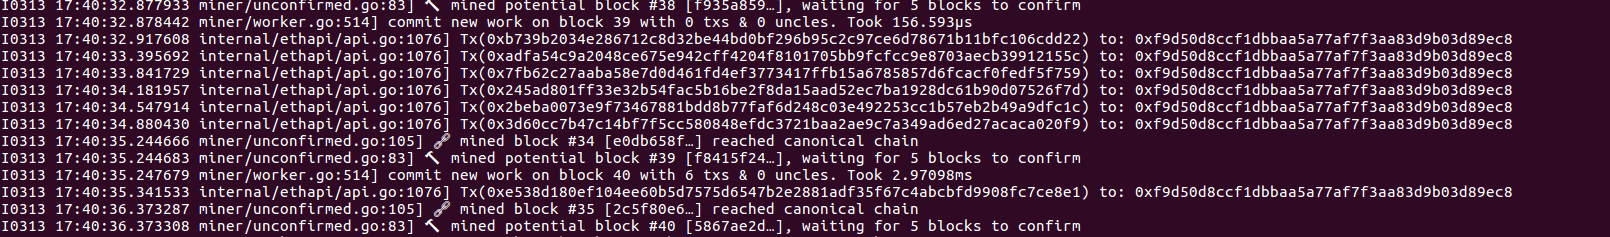
\includegraphics[width=1\textwidth]{geth_screenshot.png}
\caption{Snapshot of mining console on Go Ethereum}
\label{geth_snapshot}
\end{center}
\end{figure}

\subsubsection*{Dagger Hashimoto algorithm specifications}

This algorithm is a combination of two different algorithms namely, \textit{Dagger} and \textit{Hashimoto}, invented by Vitalik Buterin and Thaddeus Dryja respectively. 

Dagger Hashimoto uses a custom generated DAG data set, which gets updated at frequent intervals based on the blockchain metadata. Currently, the DAG is regenerated after the creation of every 30,000 blocks. The DAG is represented as a two dimensional array or a matrix with the dimensions of n * 16, where n is a large number greater than 16777186. The DAG has a depth of ten including the root level, and can have 2\textsuperscript{25}-1 values in total. For the first eight levels, every node in the DAG must have three parents that affect the value of the node. If the number of nodes at a given depth is N, then the number of nodes in the next level must be eight times larger than that i.e., 8N. For the ninth level, the value of each node in the DAG is dependent on sixteen parents and the number of nodes in the ninth level is two times that of the eighth level. The algorithm then pseudorandomly selects eight nodes, adds the nonce value to the block headers and computes a hash out of it. If the miner finds a nonce value less than 2\textsuperscript{256} divided by the difficulty amount, the PoW is solved and a block is generated. 

The following snippet, adapted from \cite{dagger}, illustrates the algorithm. In the code below, D depicts the block header value, N the nonce value, L is the depth and spread(L) refers to the number of parents a node must have depending on the depth, and || is the concatenation operator. The objective of the code here, is to find the value of k, such that the value of the function eval(D,k) is less than 2\textsuperscript{256} divided by the difficulty value.

\begin{verbatim}
spread(L) = 16
if L == 9
else 3

node(D, xn, 0, 0) = D
node(D, xn, L, i) =
  with m = spread(L)
p[k] = SHA256(D || xn || L || i || k) mod 8 ^ (L - 1) for k in [0...m - 1]
SHA256(node(L - 1, p[0]) || node(L - 1, p[1])... || node(L - 1, p[m - 1]))

eval(D, N) =
  with xn = floor(n / 2 ^ 26)
p[k] = SHA256(D || xn || i || k) mod 8 ^ 8 * 2
for k in [0...3]
SHA256(node(D, xn, 9, p[0]) || node(D, xn, 9, p[1])... || node(D, xn, 9, p[3]))
\end{verbatim}

Figure \ref{DAG_generation} shows a snapshot of DAG generation on the mining console logs of Go language implementation of Ethereum.

\begin{figure}[H]
\begin{center}
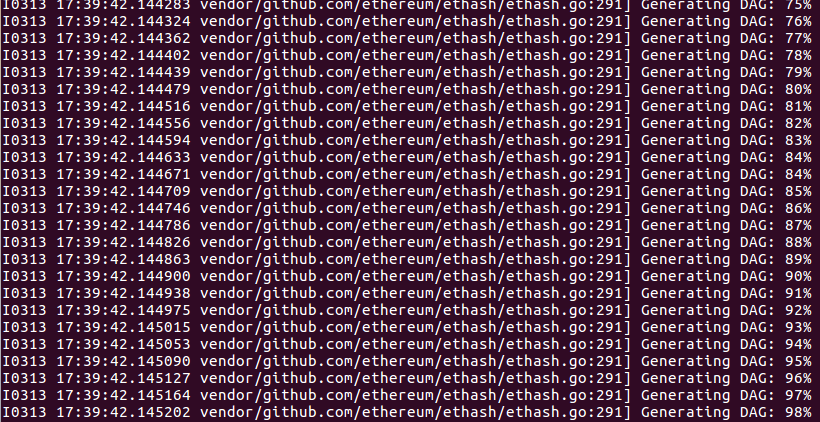
\includegraphics[width=0.9\textwidth]{DAG_generation.png}
\caption{Snapshot of DAG generation in mining console on Go Ethereum}
\label{DAG_generation}
\end{center}
\end{figure}

\subsection{Main differences between Bitcoin and Ethereum}

While both Bitcoin and Ethereum are based on the same fundamental idea of cryptography and having a distributed ledger, there are distinct differences in their technicalities and the applications they are meant for. Bitcoin uses a stack based language whereas Ethereum uses a turing complete programming language. The consensus and block approval time in case of Ethereum is about 15 to 17 seconds, which is much lower than that of Bitcoin (10 minutes). The basic build of the proof of work algorithms that Ethereum uses is a memory hard hashing algorithm called Dagger-Hashimoto, while Bitcoin makes use of the SHA-256 hash algorithm. The economic models of the two are also slightly different. The Bitcoin miners have their block creation rewards halved every four years, whereas in case of Ethereum there is no such rule of reward reduction. The way the transaction fees are levied are also very different. Ethereum uses the concept of Gas based on the computational complexity of the operations performed, and has a maximum value per block. For Bitcoins, the transaction fees is limited by the block size.

However, from a general outlook, the applications and use cases Bitcoin and Ethereum were built for are very different. The idea of Bitcoin was to replace real money with cryptocurrencies without having to depend on central authorities to trust on, such as banks and governments. Thus, Bitcoin was meant to be a transaction channel and for the purpose of storing values. Ethereum, on the other hand, was meant to act as a platform to build decentralized applications and contracts using its own currency as a medium. The primary motivation for Ethereum was therefore, to be a facilitator for the developers to build their own DApps. 

\subsection{Other Implementations}

In the big picture, it can be observed that there are two main methods a blockchain system can be built. The first being building a blockchain system by forking an existing system, and the second, building an independent system from scratch. Bitcoin and Ethereum are examples of independent systems built from scratch. Building a system from scratch is naturally pretty difficult to implement, despite some companies such as Namecoin having had reasonable success with it. The drawback such a system could have, would include communication issues between two or more applications having independent blockchains of their own. Systems that fork an existing independent blockchain system with alternative consensus rules are known as \textit{Alt-coins} or alternative coins. 

Using the first method described above, building a system on top of Bitcoin has the disadvantage of not being able to inherit the SPV system that Bitcoin uses. The current systems built on top of Bitcoin that have lightweight clients rely on a trusted server to provide them the blockchain data, which sort of defeats the purpose of having a trustless decentralised blockchain. There are also systems that are built on top of Ethereum, and target specific business needs.


\subsubsection{Systems built on the Bitcoin blockchain}
This section illustrates some of the blockchain implementations that were built as a fork of Bitcoin. 

\subsubsection*{Namecoin}
Namecoin \cite{namecoin} is the first fork of Bitcoin and uses the same proof of work algorithm. The cryptocurrency system has the capability to store data in its own blockchain transaction database. The function of Namecoin can be best described as being a name register, or the equivalent of a DNS. They also have a domain name \textit{.bit}, but it is independent of ICANN, the governing body of domain names. 

In decentralised protocols such as Bitcoin and Ethereum, the accounts have a hash like identifier such as '1AW29dp2ZCbqW5CiBCrhQYtHagUWy'. Such identifiers, though are advantageous for the purpose of being obscure enough to not be impersonated, are difficult to interact with. Namecoin solves the problem by introducing the decentralised domain system and a first to file paradigm to prevent impersonation, where the first person who registers the name succeeds and the others fail.

\subsubsection*{Colored coins}

Colored coins\cite{coloredcoin}, serves as a protocol to let people create their own cryptocurrencies, or even digital tokens on the Bitcoin blockchain. A new cryptocurrency can be issued by assigning a specific Bitcoin UTXO to a specific colour, and the users of that particular cryptocurrency would then maintain wallets containing UTXO outputs of a certain colour. They also have some special rules in case of mixed colour inputs and outputs. Simply put, color in this case is an attribute of a certain cryptocurrency, as well as its further applications. For example, certain colors could be meant for proving ownership of a car.

\subsubsection*{Metacoins}

Metacoin\cite{metacoin} is an extension on top of the Bitcoin blockchain and therefore does not inherit the SPV characteristics of the Bitcoin blockchain. Doing this provides a relatively easy to implement and low development cost process to create a consensus protocol with a possibility of having advanced features that cannot be implemented in the Bitcoin framework itself. For example, a small Bitcoin can be "labelled" as an ounce of gold, or a share in a company or even be counted as a score value in a video game.

\subsubsection*{Cryptonite - Mini Blockchain}

Cryptonite is the first implementation of the lightweight \textit{Mini-Blockchain} scheme\cite{cryptonite}. Their main intention of developing this cryptocurrency was to improve the scalability problem faced by Bitcoins. The mini blockchain scheme includes a self contained balance sheet system thereby eliminating the need to store transaction data perpetually. As a result, the maximum block size can be made larger. Even though the system has the advantage of being faster and less expensive, the drawbacks include a weakened security and less flexibility.

\subsubsection*{MultiChain}

MultiChain \cite{multichain}, a fork of Bitcoin, is a customizable and private blockchain service. Their main motivation behind building this software was to cater to large financial institutions that were not interested in using public blockchains. The multichain system also uses a randomised round robin method to add blocks onto the blockchain, and has a configurable mining process. 

\subsubsection*{Rootstock}
Rootstock\cite{rootstock}, an open source platform, is very similar to Ethereum in terms of creating smart contracts on a Turing complete smart platform, except that it utilizes the Bitcoin ecosystem to do so. The advantages to this platform are that it exists as a Bitcoin \textit{sidechain}, and is backward compatible with the Ethereum virtual machine. This means that all Ethereum contracts can easily run on Rootstock. Their biggest advantage, however, is the fact that they can be merged mined with Bitcoin, thereby making it as secure. A \textbf{sidechain}\cite{sidechain} is a separate blockchain, whose assets can be transferred to and from the main blockchain, i.e. the Bitcoin blockchain in this context. This is a promising platform because it proposes Ethereum with a Bitcoin like security. 


\subsubsection{Systems built on the Ethereum blockchain}
This section provides a brief description of some blockchain implementations forked from Ethereum.
\subsubsection*{Eris}
Eris industries (now called Monax Industries) is a blockchain application platform that caters to financial institutions and helps them deploy private blockchains for their needs. They have forked Ethereum and also employ other technologies and wrapper tools that helped them become blockchain technology agnostic. They also provide service tools around Ethereum Virtual Environment.

\subsubsection*{Hydrachain} 

Hydrachain \cite{hydrachain} is an open source platform built on top of Ethereum, and adds support for creating scalable permissioned (private or consortium) blockchains. Their main distinguishable features are the introduction of \textit{accountable validators} and \textit{instant finality} for private blockchains. Accountable validator refers to to a set of registered that propose and validate the order of transactions in the hydrachain distributed ledger. They use a byzantine fault tolerant consensus protocol that does not work with the proof of work algorithm. \cite{pbft} and \cite{pbft2} explain the practical byzantine fault tolerance protocol that Hydrachain follows, and how it does not work with PoW. There needs to be a quorum by the validators that sign the blocks, before the block is added to the blockchain. This allows for the block time to be less than a second.

\subsubsection{Independent blockchain systems}
This section gives a brief description of Blockchain implementations built from scratch.

\subsubsection*{Hyperledger}
Hyperledger\cite{hyperledger} is a project hosted by the Linux Foundation as a cross industry collaborative project. The system was designed with the enterprise architecture in mind with customizable networking rules that help different consensus protocols operate. It borrows the UTXO and script based logic from Bitcoins and uses a byzantine fault tolerant consensus protocol instead of the proof of work algorithm. In general, it most likely is sort of an umbrella system that encompasses most possible use cases to suit the blockchain industry. 

\subsubsection*{Lisk}
Lisk \cite{lisk} is a platform for decentralized applications and sidechains programmed in Javascript, and have a block time of approximately 10 seconds. They use DPoS as their consensus mechanism. They also have their own academy videos\cite{liskacademy} that teaches developers how to get acquainted with their system.

Their main idea is that every blockchain app, or the DApp equivalent of Ethereum, has its own sidechain, which helps with the scalability issues that the Bitcoin and Ethereum blockchains have been facing. \newline


\begin{table}[H]
\centering
\begin{tabular}{|l|c|l|}
\hline
\textbf{System Name} & \multicolumn{1}{l|}{\textbf{Underlying System}} & \textbf{Salient Features}                                                                                                                         \\ \hline
Namecoin             & \multirow{6}{*}{Bitcoin}                        & Decentralised domain system.                                                                                                                      \\ \cline{1-1} \cline{3-3} 
Colored coins        &                                                 & \begin{tabular}[c]{@{}l@{}}A digital asset protocol that \\ can customise the asset to suit \\ specific needs.\end{tabular}                       \\ \cline{1-1} \cline{3-3} 
Metacoins            &                                                 & \begin{tabular}[c]{@{}l@{}}A digital asset protocol that \\ adds functionality to the Bitcoin \\ protocol.\end{tabular}                           \\ \cline{1-1} \cline{3-3} 
Cryptonite           &                                                 & \begin{tabular}[c]{@{}l@{}}A mini blockchain scheme with\\ its own balance calculator.\end{tabular}                                               \\ \cline{1-1} \cline{3-3} 
Multichain           &                                                 & \begin{tabular}[c]{@{}l@{}}A private blockchain system\\ for financial institutions.\end{tabular}                                                 \\ \cline{1-1} \cline{3-3} 
Rootstock            &                                                 & \begin{tabular}[c]{@{}l@{}}A smart contract platform based\\ on Bitcoins.\end{tabular}                                                            \\ \hline
Eris                 & \multirow{2}{*}{Ethereum}                       & \begin{tabular}[c]{@{}l@{}}A smart contract platform coupled \\ with service tools for ethereum\\ virtual machine.\end{tabular}                   \\ \cline{1-1} \cline{3-3} 
Hydrachain           &                                                 & \begin{tabular}[c]{@{}l@{}}A smart contract platform with \\ accountable validators and instant\\ finality for private blockchains.\end{tabular}  \\ \hline
Hyperleger           & \multirow{2}{*}{Independent}                    & \begin{tabular}[c]{@{}l@{}}An umbrella blockchain system to \\ facilitate maximum possible use\\ cases for the industry.\end{tabular}             \\ \cline{1-1} \cline{3-3} 
Lisk                 &                                                 & \begin{tabular}[c]{@{}l@{}}A decentralised application platform\\ that makes use of sidechains for each\\ decentralised app created.\end{tabular} \\ \hline
\end{tabular}
\caption{Overview: Some blockchain implementations discussed above}
\label{blockchain_implementations}
\end{table}

\newpage
\section{Management of Internet of Things Devices}

Ericsson estimates the number of connected IoT devices to be upto 28 billion by 2021\footnote{Ericsson's prediction on their annual report: http://www.ericsson.com/res/investors/docs/2015/ericsson-annual-report-2015-en.pdf}. With the ever increasing array of communication protocols between IoT devices, there is a requirement for a transparent, yet highly secure and reliable IoT device management system. Other issues include tracking these billions of devices as well as storing the metadata they produce. 

Since this thesis involves creating a device management system for constrained IoT devices, this chapter attempts to give an overview of various existing protocols and standards, and some implementations that deal with constrained devices and their management. Furthermore, the last section in this chapter attempts to introduce what it means to use blockchains with IoT and how it can be done.



\subsection{IoT Protocols and Standards}

The term Internet of Things (IoT) was coined by Kevin Ashton in 1999, while presenting at Proctor \& Gamble. He proposed it as a link between radio frequency identification and the Internet\cite{ashton}. Semantically, it refers to identifiable networked objects or things, also called devices, virtual representations of which can be connected to each other over the internet. In other words, IoT refers to a wide variety of devices, including smart devices, systems and constrained devices, that interact and automate processes in a networked society. 

Due to so much potential in the IoT field and the growing number of devices each year, solutions are being implemented in many areas, like supply chain, farming, healthcare, home automation to name a few. But with the development, people have come to realise the limitations that come from trying to make an overwhelmingly large amount of devices, belonging to different corporations and communities, communicate with each other.

\subsubsection*{Constrained Devices}

Resource constrained devices or just constrained device, as mentioned in the IETF standard \cite{constrained}, are devices that run on very limited processing, power and storage capabilities. Such networks display many constraints such as limited bandwidth or lossy channels. Continuous data retrieval from such devices is very challenging owing to the tight limits on available power, processing resources and memory. This thesis mainly makes use of CoAP as the application layer protocol, which we will discuss about in the subsequent sections.

\subsection{Constrained Application Protocol (CoAP)}

CoAP \cite{CoAPstandard} is a lightweight User Datagram Protocol (UDP) based standardised RESTful application layer protocol, for \textit{extremely} resource constrained devices in machine to machine(M2M)\footnote{M2M communications is used for automated data transmission and measurement between devices} networks. It is designed to easily interface with HTTP for integration with the Web while meeting specialized requirements such as multicast support, very low overhead, and simplicity for constrained environments\cite{CoAPstandard}. It also widens the horizons in terms of solving M2M specific problems such as asynchronoous transfer, or reduction of message overhead, or resource discovery of constrained nodes. Common applications for CoAP include smart energy and smart building automation.


\subsection{Constrained Objects Language and CoAP Management Interface}

The combination of Constrained Objects Language(CoOl)\cite{cool} and CoAP Management Interface (CoMI)\cite{comi} is a CoAP based management protocol that uses Yet Another Next Generation (YANG)\cite{yang} modelling language to define its resources. Thus, CoMI and CoOL are adapted to low power, lossy constrained networked devices. Payloads for the information exchange are encoded using Concise Binary Object Representation (CBOR)\cite{cobr} data format, which facilitates extremely small code and message size.

The protocol is based on a client-server model. The client requests for the datastore resources and the event stream resources. The server is the provider of these resources. Figure \ref{cool_archi} illustrates the semantics of the protocol architecture. As per the standard, the implementers are free to choose the appropriate form of transport pertaining to the target applications.

\begin{figure}[H]
\begin{center}
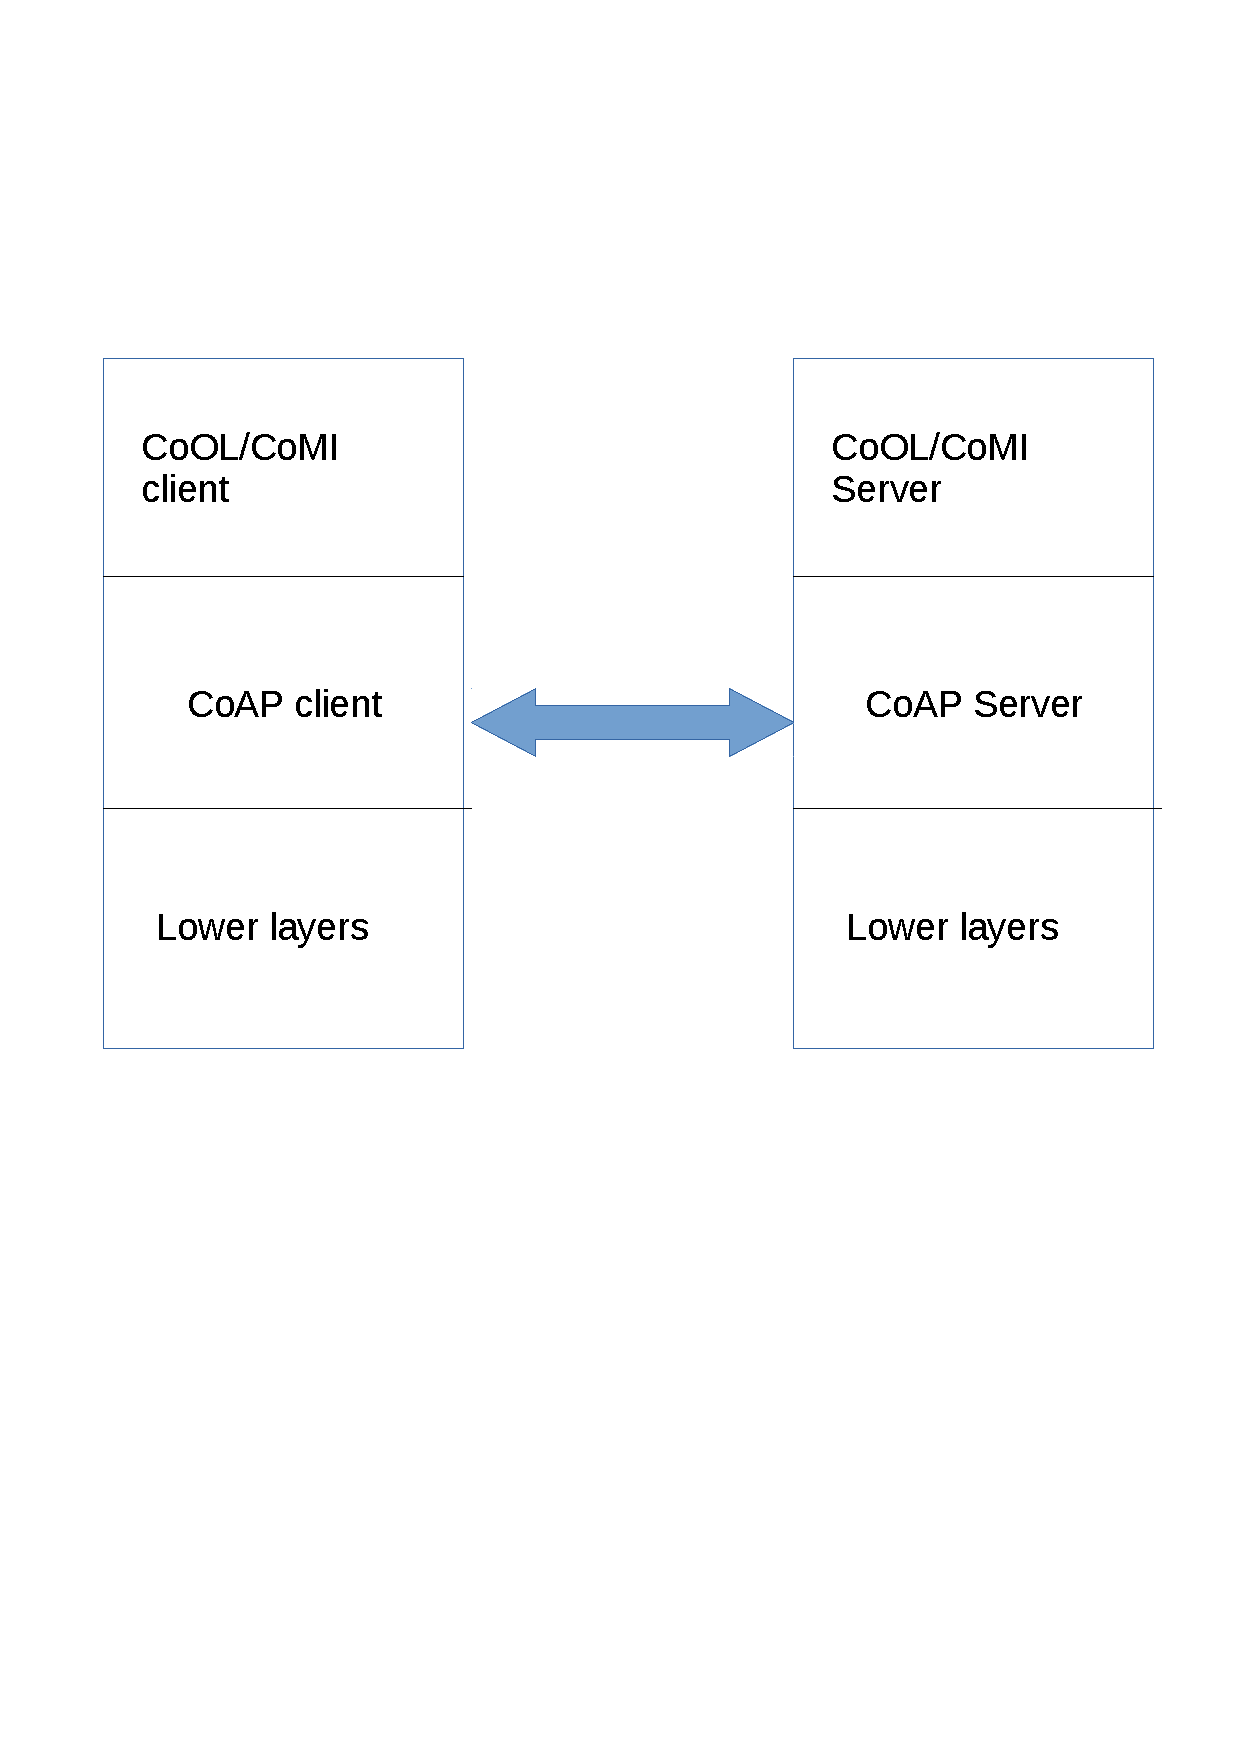
\includegraphics[width=0.8\textwidth]{cropped_CoOl.pdf}
\caption{CoOL/CoMI architecture overview}
\label{cool_archi}
\end{center}
\end{figure}


\subsection{Lightweight M2M (LWM2M)}
OMA Lightweight M2M is an important protocol from Open Mobile Alliance (OMA), for the management of constrained devices. It usually runs on top of CoAP, and therefore is compatible with any device working with CoAP as its transport protocol. The main function of the LWM2M protocol, is to provide a set of interfaces that can monitor and manage constrained devices. The aim of this standard is to facilitate a fast deployable client server system serving M2M services. 


LWM2M architecture defines three main parts namely, a \textit{Bootstrap Server, a Client and a Server}. An LWM2M \textbf{Bootstrap Server} is a configuration server for the LWM2M client before it is connected to an LWM2M server. It essentially helps the server manage access control, keying and configuration of a client. LWM2M \textbf{Clients} are usually constrained devices, and contain many LWM2M objects and their corresponding resources. The task of an LWM2M \textbf{Server} is to manage the clients through management commands e.g. execute read, update or delete commands for the resources of a particular LWM2M client. The bootstrap server is supposed to configure the access controls to connect a server to a client. 

The Open Mobile Alliance (OMA) specification \footnote{OMA specifications: http://openmobilealliance.org/} lists four logical interfaces for the server and the client to communicate with each other. They are as follows.

\begin{itemize}
\item \textbf{Bootstrap} The client sends a \textit{request} message to the bootstrap server, and the server then accordingly performs a write or delete operation on the client, in order to register or remove LWM2M servers.
\item \textbf{Client Registration} A LWM2M client registers to one or more LWM2M servers after it has been bootstrapped.
\item \textbf{Device Management and Service Enablement} An LWM2M server can send various commands to the client in order to perform actions on the resources owned by those clients. The access control object, set during the bootstrapping process, determines the policies or the set of actions the server can take on a particular client's resources. 
\item \textbf{Information Reporting} Clients can report information in the form of notifications to the corresponding servers. This can be done due to the \textit{Observe-notify}\cite{observe-notify} feature from CoAP.
\end{itemize}

An LWM2M server can carry out one or more operations, in order to manage the clients and their corresponding resources. The resources of LWM2M clients are grouped into various objects. The format of these objects is specified by the IP Smart Objects (IPSO) Alliance \footnote{IPSO Alliance: http://www.ipso-alliance.org/}. 

Figure \ref{lwm2m} depicts the architecture of LWM2M protocol.

\begin{figure}[H]
\begin{center}
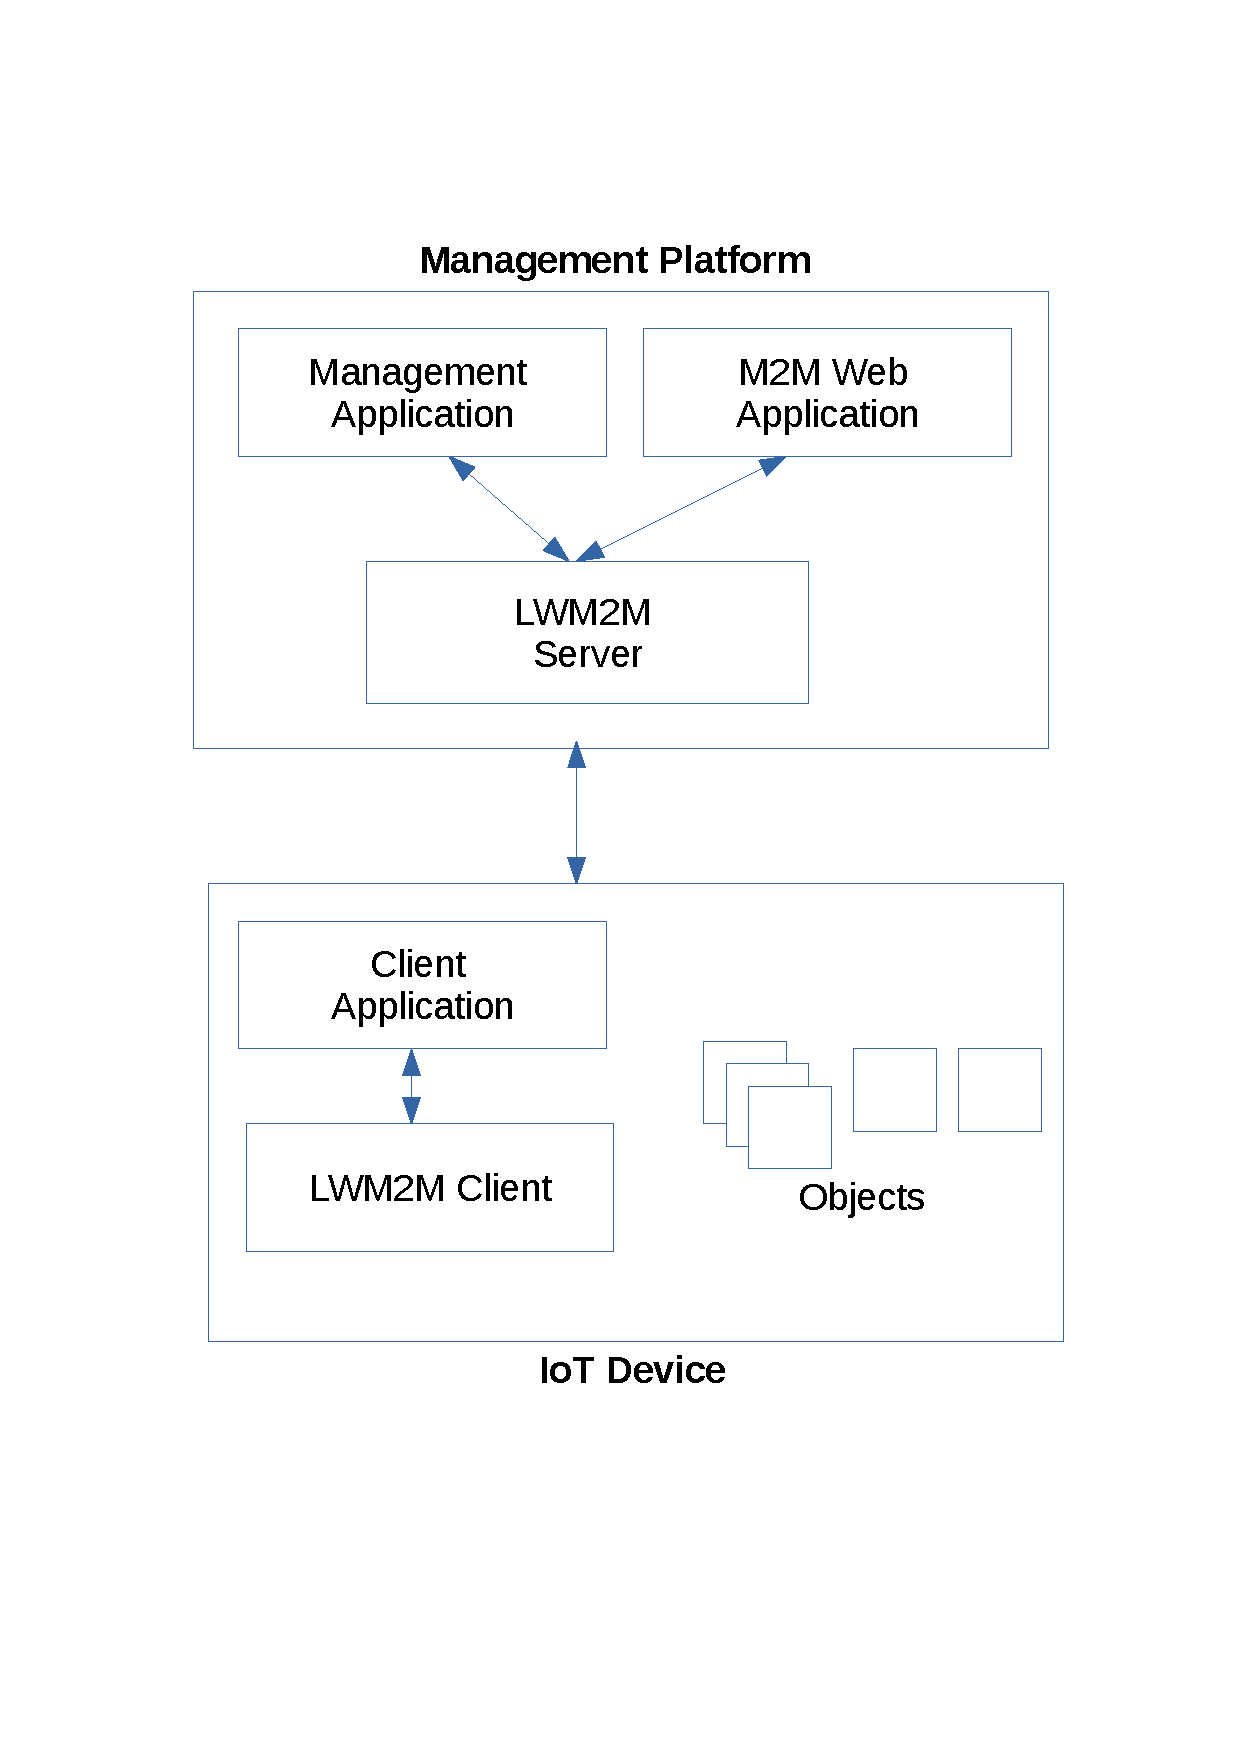
\includegraphics[width=0.7\textwidth]{cropped_lwm2m.pdf}
\caption{Architecture of Lightweight M2M}
\label{lwm2m}
\end{center}
\end{figure}

\subsubsection{Device Management Implementations for IoT using LWM2M}
\subsubsection*{Eclipse Leshan}
Leshan\footnote{Leshan project: https://github.com/eclipse/leshan} is an open source Java implementation of OMA LWM2M server and client. The project helps develop a customisable LWM2M client and server, and already comes with a demo bootstrap server, LWM2M server and LWM2M client.  
\subsubsection*{Eclipse Wakaama}
Wakaama \footnote{Wakaama project: https://github.com/eclipse/wakaama} is a C language implementation of the OMA LWM2M server and clients. The project also provides some example demo applications that test the bootstrap server, LWM2M server and client capabilities of Wakaama.

\subsection{IoT on Blockchains}

From a generic perspective, it can be said that a blockchain is an immutable ledger of transactions. Through this, millions of IoT devices can be tracked thereby enabling secure co-ordination and communication between devices. The fact that blockchain is tamper proof and operates in a trustless environment, makes it extremely difficult to manipulate.

One way to use IoT on blockchains, would be to consider each IoT device as a blockchain node. Since the use of consensus algorithms in blockchains enable it to operate in a trustless environment, the IoT devices would not need to trust each other inherently. The devices can then co-ordinate with each other through a common network, despite having been produced by different manufacturers, or having incompatible softwares. If this can be done at a global level, then it would result in a web based user centric behaviour, as opposed to the current behaviour centred mainly around devices. But sometimes when IoT devices are constrained or incapable of storing a copy of blockchain, depending on their capacity, it is possible to either use them as lightweight clients, or have a higher capacity device as their blockchain representative node.

This kind of an arrangement could lead to several use cases that are hard to acheive at the current levels of interoperability between IoT devices. Some examples include blockchain acting as a "phone-book" to let machines find each other\footnote{Implemented by onename: https://onename.com/}, creating a verifiable record of the usage of industrial medical devices\footnote{Implemented by tierion: https://tierion.com/} or a washing machine becoming a semi-autonomous device capable of managing its own supply of detergents and other parts\footnote{Prototype implemented by IBM}.

 

\newpage
\section{Design and Implementation of Proof of Concept} 
\label{Section:Implementation}

This chapter describes the small scale prototype that was developed for the management of constrained IoT devices. Section \ref{Section: Rationale} describes why a certain implementation of Blockchain was chosen to implement the prototype. Section 5.2 describes the architecture and implementation of the system.

\subsection{Rationale behind choice of technology} \label{Section: Rationale}
To be able to create a peer to peer distributed system in a trustless environment and still guarantee security, were of paramount significance for the prototype. Other factors such as ease of implementation through developer communities, and good documentation, were also considered while choosing the technology for the proof of work. 

The creators of Bitcoin purposefully did not want to have loops in their scripting system in order to make it deterministic. That makes it easier to know exactly how a particular program ends. But for this project, it was important that we make use of loops so that we can store pertinent data in certain data structures and then iterate through the data. Therefore, Bitcoin was not chosen due to the absence of support for loops, and a very rudimentary scripting language\footnote{Bitcoin Script: https://en.bitcoin.it/wiki/Script}. Ethereum, on the other hand, uses a Turing complete language for development of decentralised applications. 

Bitcoin also has relatively limited storage capabilities and is intended only as a cryptocurrency rather than being a decentralised application platform. The only way data can be transferred between two Bitcoin accounts at the moment, is through transactions. The data passed in such circumstances is public and therefore, is at a risk. 

Another advantage of Ethereum that was taken into account, while choosing the technology to work with, was that the Bitcoin blockchain has a hard limit of 1 megabyte for a block size, whereas the Ethereum blockchain does not. However, Ethereum does have a limit to how much total gas can be spent per block, which is usually 1.2 times the exponential moving average. The gas limit on the Ethereum was more convenient to handle in comparison with the hard limit of 1 MB on Bitcoin blocks.

\subsection{Architecture} 
The prototype that has been implemented for discussion in the thesis was designed to mitigate the issues associated with management of a large number of constrained IoT devices. 

This part presents an overview of how the system is designed to work, high level architectural design and implementation of a blockchain based access management system for IoT devices. The basic application design is illustrated in Figure \ref{system_design}. \newline

\begin{figure}[H]
\begin{center}
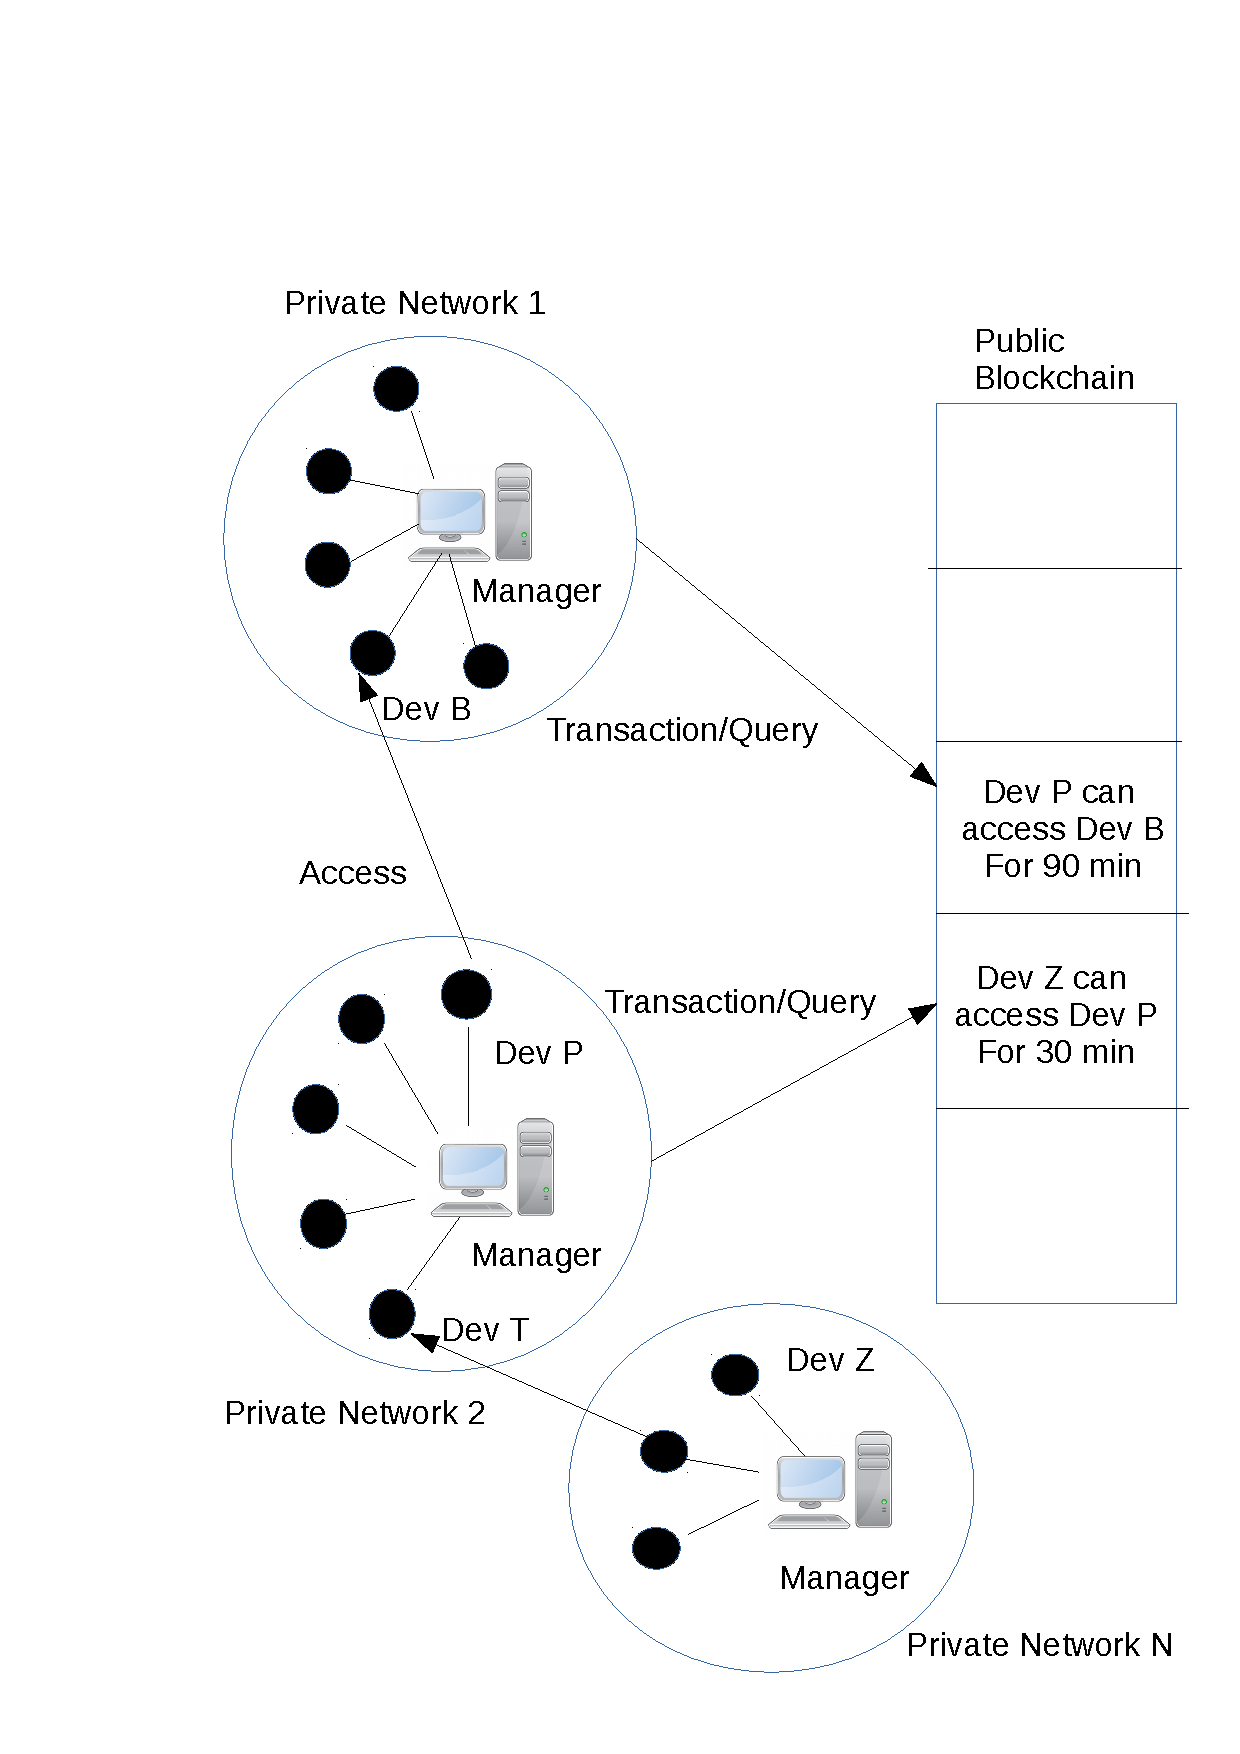
\includegraphics[width=0.6\textwidth]{cropped_overview.pdf}
\caption{Overview of the system design}
\label{system_design}
\end{center}
\end{figure}

Since the IoT devices are largely constrained, they do not have the ability to store a copy of the blockchain in their system, thereby not participating in the blockchain network themselves. They instead, have an administrator node connected to the network, that we call \textit{Managers}. The second set of actors, called \textit{Clients} are nodes that do not have the rights to manage a certain device but want to query about their states. Figure \ref{use case} presents the use case diagram showing the roles played by the actors involved in the system. \newline 

\begin{figure}[H]
\begin{center}
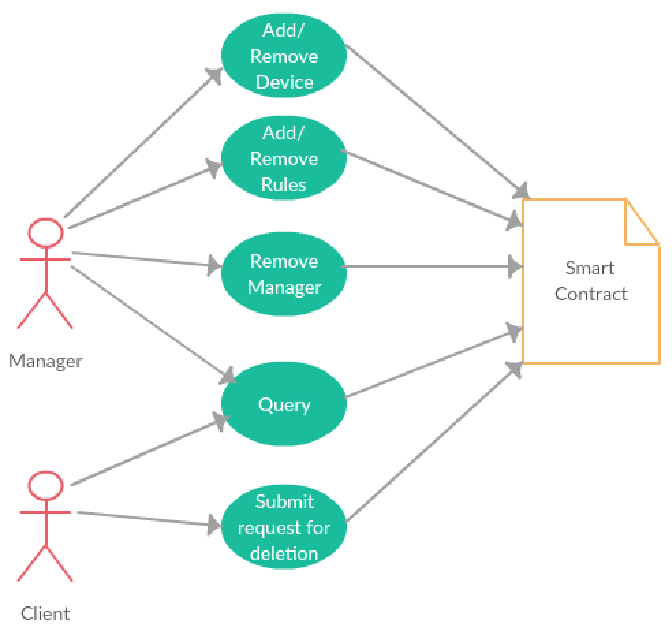
\includegraphics[width=0.7\textwidth]{uml1.pdf}
\caption{Use case diagram for the actors}
\label{use case}
\end{center}
\end{figure}

The system makes use of the Ethereum blockchain with a custom genesis block. Ethereum nodes support a node discovery feature, also called the discovery protocol. In this protocol, the nodes continuously try to find peer nodes to connect to, until the criteria of the number of peers required, as specified by the \textit{--maxpeers} flag, is met. Another way for the peers to find each other, is by manually adding the identity of the corresponding peer nodes. In the latter case, the nodes that are manually connected are called \textit{Static} nodes. In this system, we use the static connection to avoid unpredictable situations. 

Figure \ref{system_design} illustrates different managers managing their own sets of constrained devices, operating under their respective private networks and firewall configurations. Before registering the constrained devices to the blockchain, the manager adds itself as a \textit{manager} on the blockchain, by broadcasting a registration \textit{transaction}. Upon verification of this transaction by the miners, it is added to the blockchain. The constrained devices then send an identity registration message to their respective managers, and in turn are registered in the blockchain by the manager by the way of broadcasting a registration transaction.
Now as shown in Figure \ref{system_design}, constrained device Dev P, from Private Network 2 needs to access certain resources of Dev B from Private Network 1. Dev B's manager sends a transaction to the blockchain announcing the rule "Dev P can access Dev B for 90 minutes". The miners check the transaction, and a rule is established on the blockchain. Dev P can now access Dev B.

\subsubsection{Data flow in the system}
The proof of concept created to address the characteristics of our system consists of four separate components namely, the contract creator, the client, the manager and the Ethereum smart contract. The functions of each component have been broadly illustrated in Table 6. Figure 11 illustrates the block diagram showing how the different components interact. \newline

\begin{table}[H]
\centering
\label{application functions}
\begin{tabular}{|l|l|}
\hline
\textbf{Application} & \textbf{Function}                                                                                                                                                           \\ \hline
Contract creator     & \begin{tabular}[c]{@{}l@{}}an API that compiles and deploys \\ the smart contract to the blockchain\end{tabular}                                                            \\ \hline
Client               & \begin{tabular}[c]{@{}l@{}}queries the smart contract and submits \\ requests for the Manager to approve\end{tabular}                                                       \\ \hline
Manager              & \begin{tabular}[c]{@{}l@{}}registers and deregisters device identity, \\ adds and deletes rules corresponding to \\ the device, and queries the smart contract\end{tabular} \\ \hline
Smart Contract       & \begin{tabular}[c]{@{}l@{}}includes the logic to store and remove \\ all the data and permissions based on \\ the role.\end{tabular}                                        \\ \hline
\end{tabular}
\caption{Functions of the components}
\end{table}

\begin{figure}[H]
\begin{center}
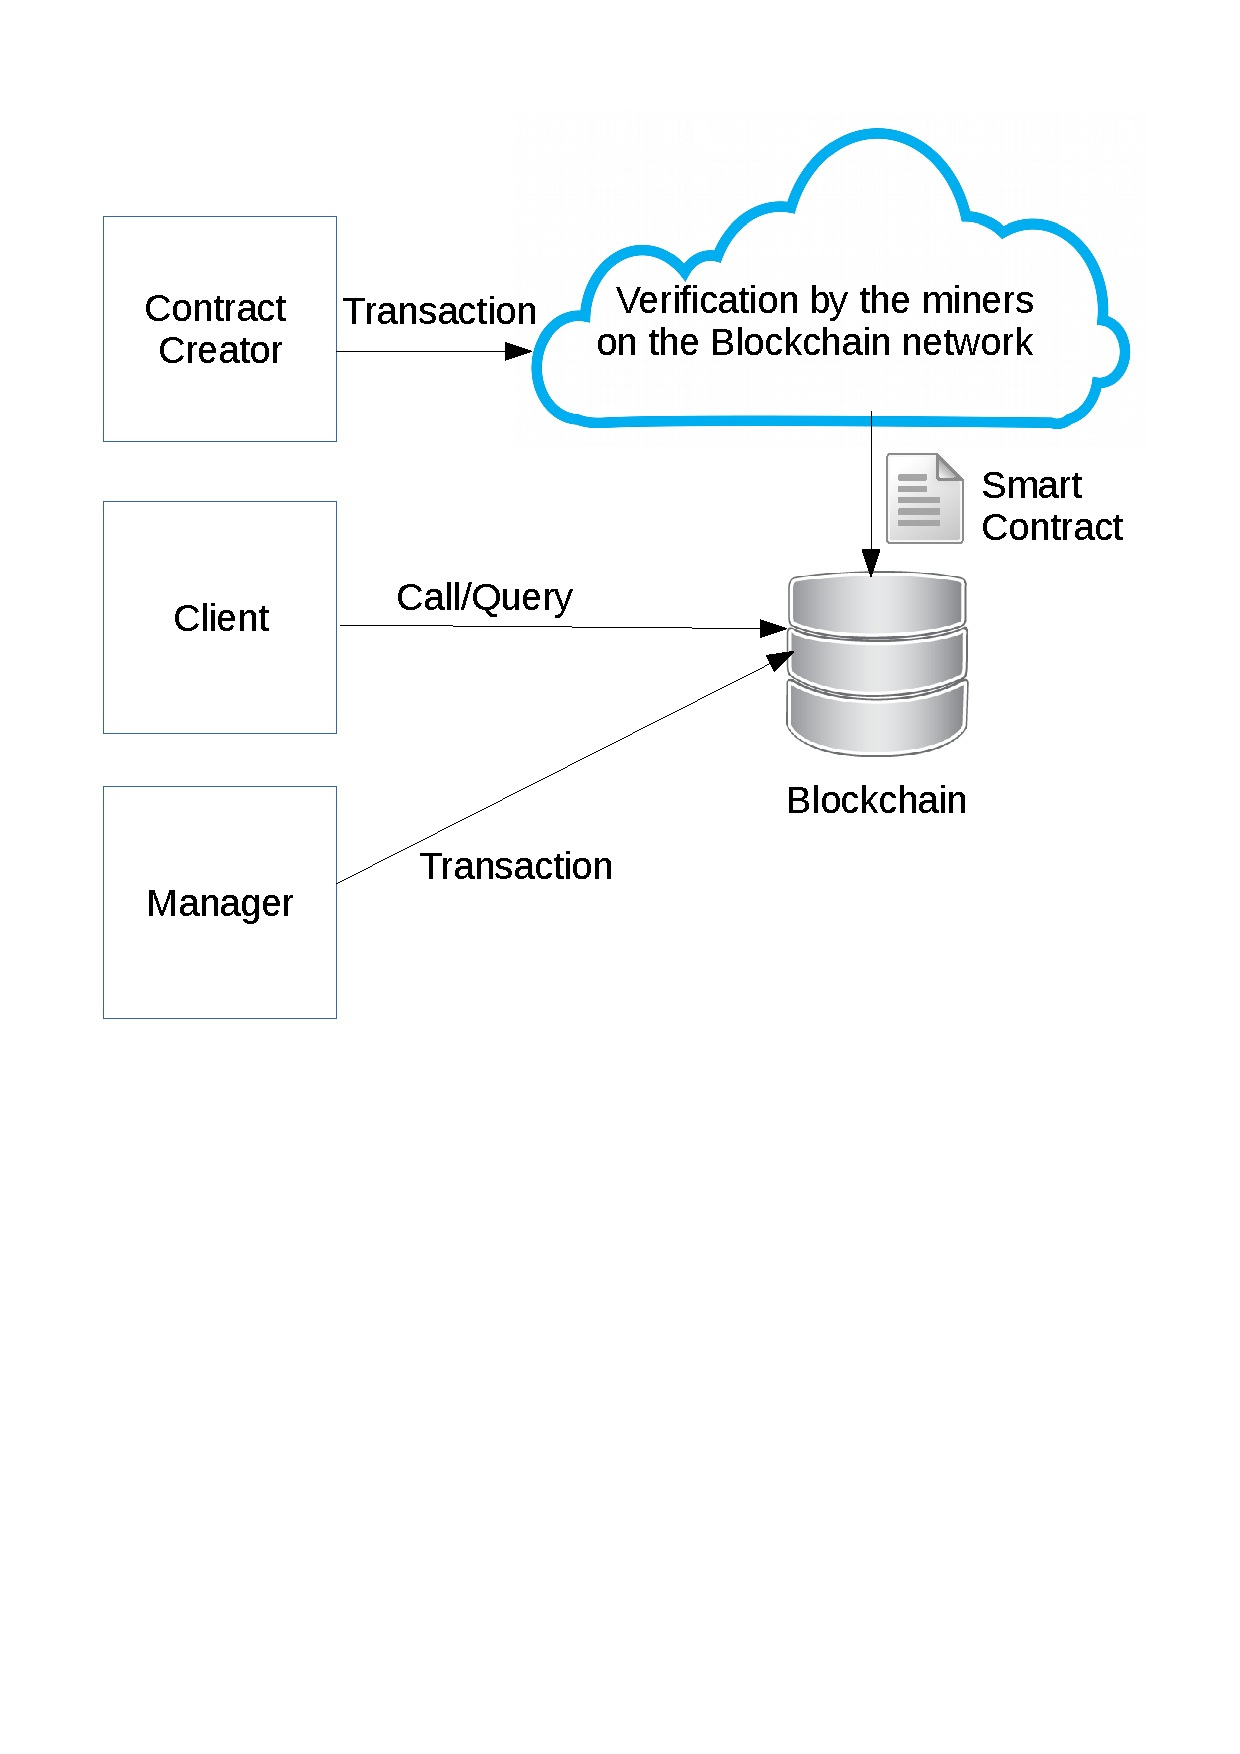
\includegraphics[width=0.9\textwidth]{cropped_component_diagram.pdf}
\caption{Overview of how the different components interact}
\label{proof-of-concept}
\end{center}
\end{figure}


\subsubsection{Component: Contract Creator} \label{component:contract_creator}
This application consists of a back-end written in NodeJS\footnote{NodeJS: A server side JavaScript based framework. https://nodejs.org/en/}. It can be hosted on a webserver, or locally on a node that participates in the blockchain network. JavaScript was chosen because the application was intended to be an application programming interface (API) that can then be integrated with client. The main motivation behind developing this application was to automate the smart contract creation process. 

The application takes the smart contract code as an input, compiles it and deploys it to the blockchain network. This deployment is broadcast as a \textit{transaction} in the blockchain. The smart contract then goes through the validation process on the network and when correctly verified, gets stored into the blockchain forever. The detailed description of the functions used in the contract creator application have been described in \textit{Appendix 1}.

\subsubsection{Component: Manager}
Managers are the main actors in the system. They have the ability to make changes to the data stored on the smart contract memory. Depending on the permissions, a manager can perform the following operations on the smart contract.
\begin{itemize}
\item Register and de-register (if needed) the identity of a constrained device to the blockchain
\item Add and remove rules corresponding to the devices they manage, to the blockchain
\item Query the blockchain
\end{itemize}

These operations are explained in detail in the smart contract subsection.

A manager is responsible for a certain set of devices, that it alone can register to the blockchain. It also adds access rules corresponding to the devices it manages, such as which constrained device can access a specific resource in a device it manages and for how long, as illustrated in Figure \ref{system_design}.

All managers host a personal copy of the blockchain i.e., they act as full nodes. They can store it in any kind of network accessible storage, privately hosted, on the cloud, decentralised storage such as Swarm\footnote{Swarm: A decentralised content distribution platform. More information at http://swarm-gateways.net/bzz:/theswarm.eth/} or IPFS\footnote{IPFS: A peer to peer distributed web storage system. More information at https://ipfs.io/} or other types of storage. For the sake of simplicity, it has been presumed that all managers also act as miners in the system. This ensures the safety of the system in case of a malicious manager.

\subsubsection{Component: Client}

Clients include the managers that do not have access to a certain device, but want to query the system about the manager of a specific constrained device, or want to check whether one constrained device can access another one. The clients only have sort of a read-only access and do not have the permission to modify the system on behalf of devices they do not manage. They can request for a rule to be deleted or a manager to be deleted, which is approved by the manager.

The front end or the client, shown in Figure \ref{dapp}, uses a JavaScript library called React\footnote{React: A JavaScript library for building user interfaces. https://facebook.github.io/react/} and is needed to trigger the JavaScript back-end.  

The back-end is a JavaScript file representing the client application in the proof of concept. The client can be hosted on a webserver, or on a decentralised storage such as Swarm or IPFS, or locally on a server that participates in the blockchain network. It may be used by all the participants on the network to communicate with the smart contract, on successful contract creation and deployment by the \textit{Contract Creator}. The client interacts with the smart contract memory through the \textit{Web3} library of JavaScript and can do the following things based on the permissions.

\begin{itemize}
\item Query if a device or a rule exists in the blockchain
\item Query if a device has a certain manager
\item Submit a request to delete a rule or manager corresponding to a device 
\end{itemize} 


\begin{figure}[H]
\begin{center}
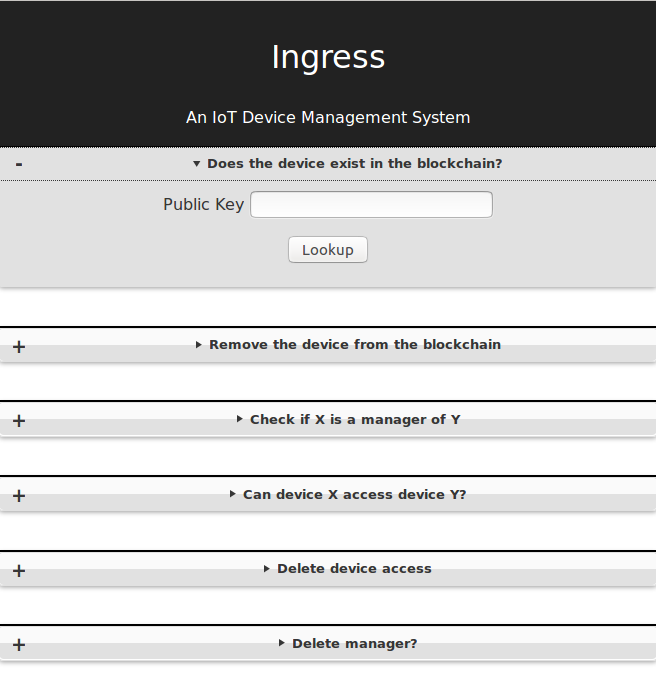
\includegraphics[width=0.9\textwidth]{ingress.png}

\caption{The front end of the Client}
\label{dapp}
\end{center}
\end{figure}
A description of the libraries used by the Client JavaScript can be found in the \textit{Appendix 3}.


\subsubsection{Component: Smart Contract}

As discussed earlier in Section \ref{Section:Smart_Contracts}, a smart contract is a distributed application that is a part of the blockchain, and is therefore hosted on all the nodes connected to the blockchain network. The smart contract has been coded in Solidity programming language. The Solidity files end with a ".sol" extension and need to be converted into the bytecode format for it to be understandable by the Ethereum Virtual Machine. The Contract Creator component, described in Section \ref{component:contract_creator}, takes care of converting the solidity code into a format that can be read by the EVM and deploys it into the Ethereum blockchain.

On deployment, the smart contract is assigned an Ethereum contract address. If any node in the Ethereum network wants to communicate with the smart contract, they do so by passing messages to its address. The messages could be of the form of a \textit{Transaction} or a \textit{Call}. Transaction messages are sent when the nodes require to store information pertinent to identities or access information of a specific device. A call is made when nodes want to query the state of a device at a given time. The following paragraphs briefly explain some of the nuances of the Solidity programming language and the functions of the smart contract. Figure \ref{smart contract} shows the general architecture of the smart contract implemented for the prototype.\newline




\begin{figure}[H]
\begin{center}
\includegraphics[width=0.7\textwidth]{architecture_sc.png}
\caption{Simplified architecture of the smart contract}
\label{smart contract}
\end{center}
\end{figure}

The implemented smart contract consists of a various functions corresponding to certain features. The Manager component has access to all the features in the smart contract, provided the actions performed by the manager are on behalf of the devices it manages. The features have been explained in the following paragraphs.

The custom data type refers to the 'Struct' data type defined in the solidity language. The struct data type facilitates grouping of different data types together in contiguous memory locations, thereby combining them to form a unified data type. In this case, the constrained device information, the manager information, and the rule details are stored in three different structs. When a registration transaction is made, the registration information goes through certain checks based on the logic of the smart contract, and is stored in the Data Store. Solidity uses a non iterable data structure called \textit{Mappings} to store data. Mappings are data types that are declared as

\begin{verbatim}
mapping(Key_type=>Value_type)
\end{verbatim}


Here the Key\_type can be any low level data type in solidity. A Key\_type cannot include a mapping, a struct, a contract, a dynamically sized array, or an enum. But the Value\_type can include everything including other mappings. These Mappings may be described as hashtables, except for the fact that the key type is not stored in the mapping itself, rather the key type's hash is used to look up the value.

The smart contract has several functions, a description of which can be found in the \textit{Appendix 2}. The subsequent sections provides an explanation of the main tasks implemented by the smart contract.

\subsubsection*{Device Identity Registration and De-registration}
The identity registration operations register a management node or a constrained device into the system. This operation requires a public-key encryption system to verify the identity of the nodes before adding them into the blockchain. On verification of identities, the manager adds the devices it manages to the system and itself as its manager, which in turn generates a transaction, thereby storing the information to the blockchain upon verification by the miners. Both the operations consume a certain amount of \textit{gas} and a transaction fee for the miners. 

If needed, the manager can also de-register itself or a device registered to it. It may be noted however, that a manager can only de-register itself when it has no corresponding constrained devices to manage.

\subsubsection*{Adding and Revoking Rules}
The rule operations facilitate adding or removing some secure rules into the blockchain. These rules involve granting or denying the access rights between two constrained devices. The manager adds or removes the rules corresponding to the devices it manages. These rules specify what resource a particular devices has access to, what type of access it has and for how long. Typically, the access types vary between read, write and both. A previously added rule can also be modified and updated. 

The revocation of rules is also done by the manager, for the constrained devices it manages. Both addition and revocation of rules generate a transaction charging a certain amount of \textit{gas} and transaction fee, which is then stored in the blockchain upon verification by the miners. A depiction of how a rule is added to the smart contract can be seen in Figure \ref{rule}. \newline

\begin{figure}[H]
\begin{center}
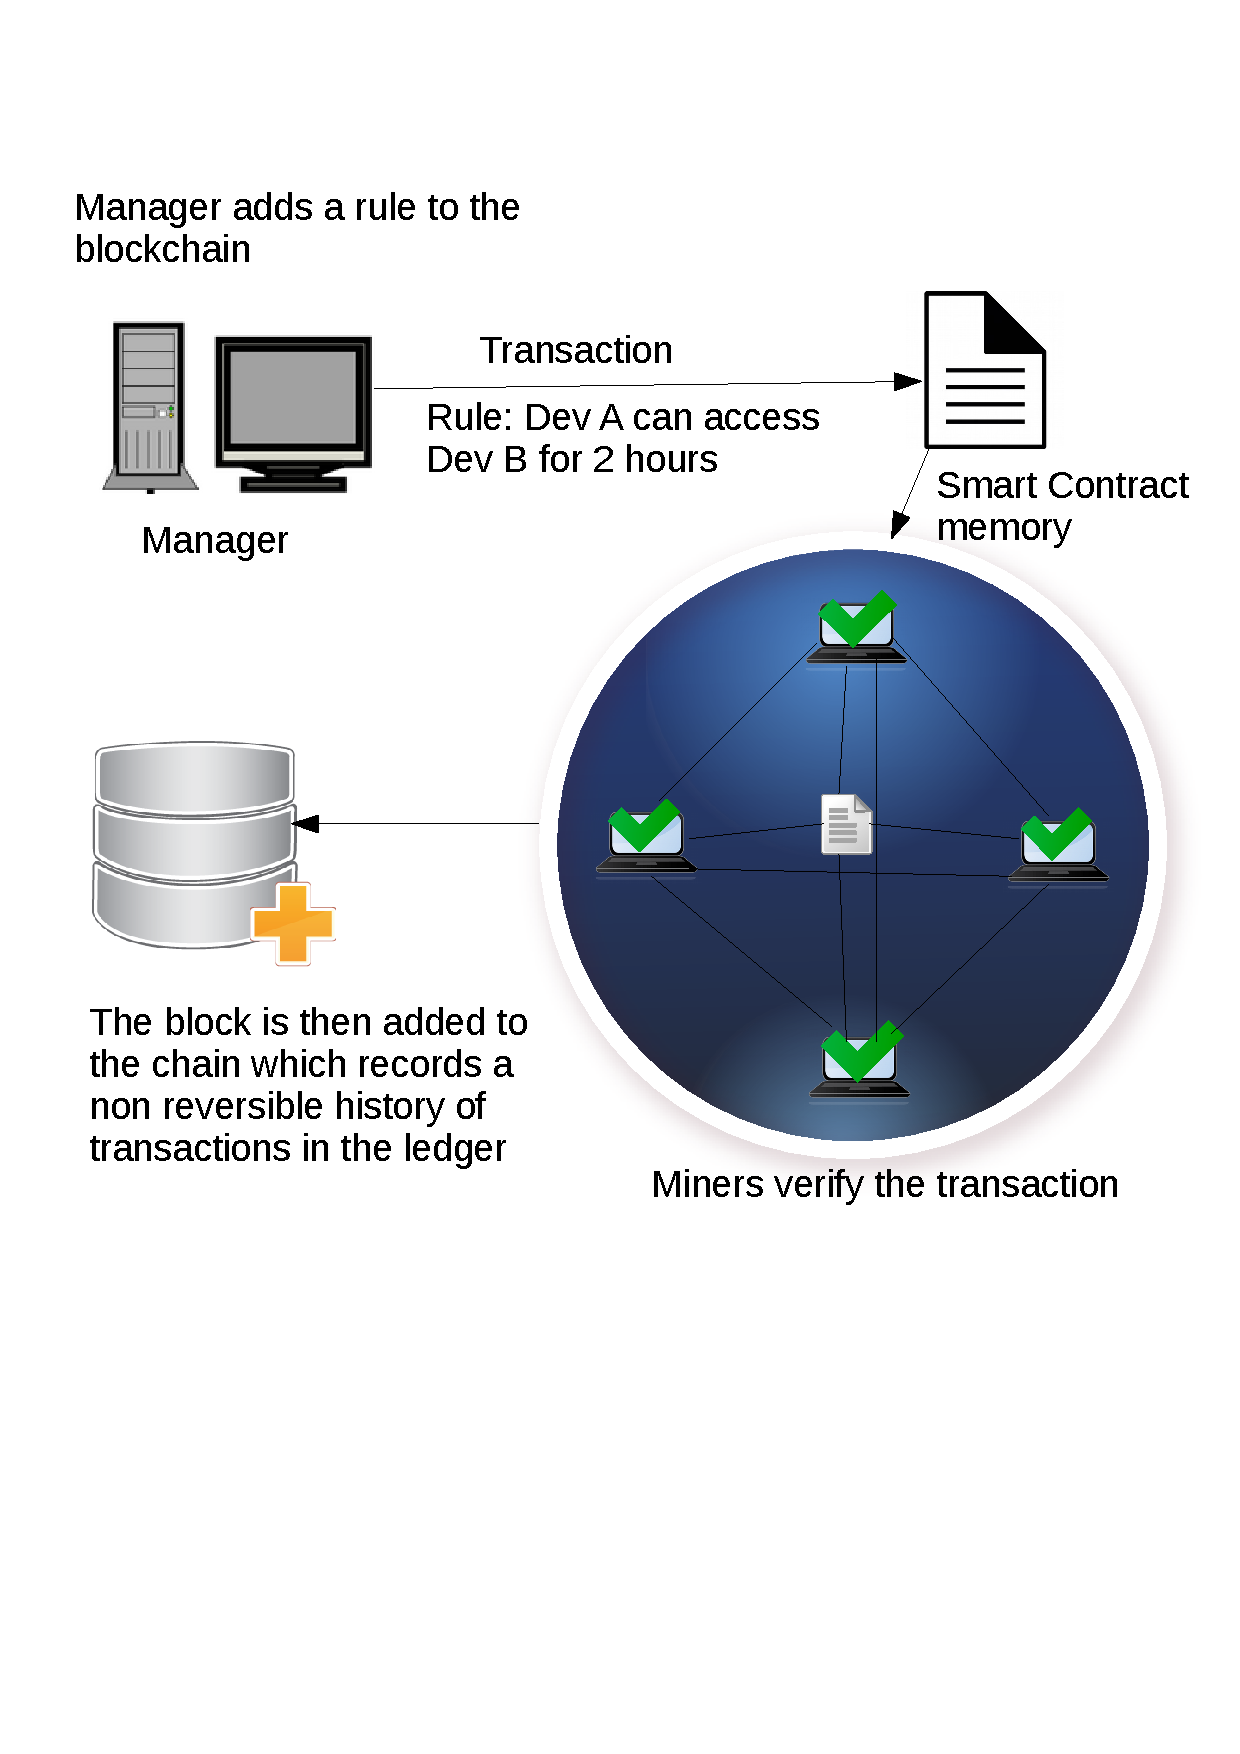
\includegraphics[width=0.8\textwidth]{cropped_rule.pdf}

\caption{Overview: How a rule is added to the smart contract}
\label{rule}
\end{center}
\end{figure}

\subsubsection*{Querying the Blockchain}
This operation queries whether one constrained device has access to certain resources in another device. Any node connected to the blockchain network can access this information in a read only manner. This operation is only meant to query the access information, and does not send out a transaction every time a client queries. This functionality in Ethereum is called \textit{Call}. A Call request invokes a function in a smart contract and gets a return value. This operation therefore, does not require any \textit{gas} or any sort of transaction fee, since it does not need to be mined.

\newpage

\section{Evaluation}
This chapter presents the evaluation of the implemented proof of concept system. The evaluation primarily refers to the assessment of the system to better understand its capabilities, and to determine whether the system meets the expected requirements.

This chapter is organised as follows. Section \ref{Section: Test Methodologies} introduces some important software testing methodologies, used during and after development of the system. Section \ref{Section: Test Environment} briefly describes the test environment and provides information on the hardware capabilities and network conditions used for the development and evaluation. Section \ref{Section: Latency} lists the metrics and the result of the evaluation experiments. Section \ref{Section: Security Analysis} analyses the security aspects of the system, and Section 6.5 briefly talks about the limitations of Ethereum Blockchains in general, as well as the proof of concept system.

\subsection{Test Methodologies} \label{Section: Test Methodologies}
Testing Methodologies are approaches used to test products to ensure they function as expected. There are many different testing methodologies depending on the stage of development. They can be broadly classified into \textit{Functional} and \textit{Non functional} testing methodologies.

\subsubsection{Functional Testing}
Functional Testing of a system refers to a kind of \textit{black box testing} meant to examine the system's external workings, according to business requirements. Black box testing is the method of testing wherein the internal workings of the system are not required to be known. It typically involves identifying the features the system is expected to perform, and determining whether the outputs match the expectations. This thesis uses two main kinds of functional testing namely, system testing and acceptance testing. \textit{System testing} includes testing the entire system for errors and bugs, and \textit{Acceptance testing} involves making sure that all the functionalities work according to expectations. 

To conduct a functional test on the smart contract, a development and testing tool called Truffle\footnote{Truffle github: https://github.com/ConsenSys/truffle} was used. It has a built in smart contract compilation system coupled with an automated contract testing framework that made the unit testing relatively convenient.

\subsubsection{Non Functional Testing}
Non functional testing requires that the system be tested against defined technical qualities some of which include \textit{Performance}, \textit{Usability}, \textit{Security} and \textit{Vulnerability} testing. This chapter mainly focuses on the non functional aspects of testing since it is of more importance, in this thesis, to understand the internal workings of the system. In the subsequent sections, there will be more discussion about the non functional testing methods and an explanation of the results obtained as a result of these non functional tests.
\subsection{Test Environment} \label{Section: Test Environment}
\subsubsection{Hardware}
The test environment consists of a host machine and an Ethernet connection. The host machine is a server running a 64-bit Ubuntu Xenial 16.04.1 LTS operating system. The processor has 8 multithreaded cores and an Intel Core i7-4800MQ processor with a maximum clock speed of 3 GHz, and a RAM of 16 GB. Each client or miner is run as a separate virtual \textit{Docker\footnote{Docker: https://www.docker.com/}} container on the host. A 240 GB Solid State Drive (SSD) was used to prevent storage disk's bottleneck issues. A 1 GbE connection has been used to evaluate the proof of concept. The network conditions are kept constant, and no external tools are used to modify the network latency or packet loss, as evaluation over different network situations is not included in the scope of the thesis.

\subsubsection{Docker Containers}
An open source software called Docker has been utilised to simulate a real world distributed system. Docker containers are a lightweight way to package a node with all the necessary runtime dependencies, and isolate it from the underlying infrastructure, i.e. the Linux kernel. Therefore, docker containers guarantee that the nodes always run in the same way. 

Docker was chosen over virtual machines, because of its lightweight nature and faster boot time due to the isolation. It also allows a very effective memory and CPU resource allocation system that was very useful for the evaluation of the proof of concept. 

\subsubsection{Testbed configuration}
This section explains an overview of the testbed used to evaluate the performance of the blockchain based system developed to manage access configurations for IoT devices. 

The system uses a private Ethereum blockchain for evaluation purposes. There are two main types of nodes used in the configuration namely, a \textit{bootnode} and \textit{managers}. As discussed earlier, Ethereum nodes support a node discovery feature, wherein they look for other peers on the network to connect to. In this case, a node that acts as a connection facilitator for the rest of the network, called a bootnode, has been used to achieve the peer connection. In practice, the main public Ethereum network is also served by three bootnodes hard-coded into the Ethereum client. The test configuration also includes six miner nodes, also called managers. The purpose of the managers has already been discussed in Section \ref{Section:Implementation}.

\subsection{Latency and Throughput Evaluation} \label{Section: Latency}
Theoretically, Ethereum does not have any upper limit on the number of transactions that a block can accommodate. When a miner tries to fit in transactions worth more than the block gas limit, the block gas limit gradually adjusts itself. In practice, however, there are many factors that influence the throughput and the latency of a blockchain network. For example, clients that are big machines with plenty of bandwidth and processing power will have a higher threshold for throughput whereas smaller devices will have a lower throughput. This evaluation attempts to exhibit how the proof of concept system behaves when the CPU processing and memory are varied. 

\subsubsection*{Evaluation Methodology and Results}
It is imperative to understand the state of the system before, during and after the evaluation is conducted, since the results depend on it to a great extent. The evaluation set-up involved setting up six miners and a bootnode on Docker containers. The role of the bootnode was to aid in peer discovery for the miners. The bootnode dynamically generates an Ethereum address, which the miners connect to, in order to find each other. The official Ethereum image \textit{ethereum/client-go\footnote{Ethereum Docker image: https://hub.docker.com/r/ethereum/client-go/}} was used on each Docker container. 

The initial bandwidth between each pair of Docker containers was examined, to rule out those bottlenecks. The bandwidth, measured using the Linux tool called \textit{iperf}\footnote{iperf:https://iperf.fr/}, averaged out to 14.6 Gbits per second. The memory and CPU consumption of the physical machine as well as every container before and during the tests were also compared. A tool called \textit{sysstat\footnote{sysstat: System performance tool for Linux. For more information: https://github.com/sysstat/sysstat}} was used to measure the performances of each Docker container and the physical host at every stage. To ensure that unnecessary processes don't interfere with the evaluations, they were terminated.

After the private blockchain was connected, the CPU quota and the memory values of each Docker container was changed to take the readings. The difficulty level for block creation was initially kept low to see if it would adjust gradually. 60 transactions of the same size and type were pushed to the blockchain each time. This was done to keep the transaction variables constant, and to check the amount of time all the nodes would take to process the transactions and reach a consensus. Due to the sheer number of steps involved in getting the system up and running, bash and javascript scripts were used to automate the process.


\begin{table}[H]
\centering
\begin{tabular}{llllllll}
\hline
\multicolumn{1}{|l|}{}                        & \multicolumn{1}{l|}{}             & \multicolumn{6}{l|}{\textbf{Time per 60 transactions (seconds)}}                                                                                                                                                            \\ \hline
\multicolumn{1}{|l|}{\textbf{CPU Quota (\%)}} & \multicolumn{1}{l|}{\textbf{RAM(GB)}} & \multicolumn{1}{l|}{\textbf{Run1}} & \multicolumn{1}{l|}{\textbf{Run2}} & \multicolumn{1}{l|}{\textbf{Run3}} & \multicolumn{1}{l|}{\textbf{Run4}} & \multicolumn{1}{l|}{\textbf{Run5}} & \multicolumn{1}{l|}{\textbf{Run6}} \\ \hline
\multicolumn{1}{|l|}{\textbf{100}}            & \multicolumn{1}{l|}{\textbf{16}}  & \multicolumn{1}{l|}{31}            & \multicolumn{1}{l|}{36}            & \multicolumn{1}{l|}{37}            & \multicolumn{1}{l|}{36}            & \multicolumn{1}{l|}{40}            & \multicolumn{1}{l|}{38}            \\ \hline
\multicolumn{1}{|l|}{\textbf{}}               & \multicolumn{1}{l|}{\textbf{8}}   & \multicolumn{1}{l|}{73}            & \multicolumn{1}{l|}{69}            & \multicolumn{1}{l|}{85}            & \multicolumn{1}{l|}{71}            & \multicolumn{1}{l|}{69}            & \multicolumn{1}{l|}{75}            \\ \hline
\multicolumn{1}{|l|}{\textbf{}}               & \multicolumn{1}{l|}{\textbf{4}}   & \multicolumn{1}{l|}{77}            & \multicolumn{1}{l|}{75}            & \multicolumn{1}{l|}{87}            & \multicolumn{1}{l|}{85}            & \multicolumn{1}{l|}{77}            & \multicolumn{1}{l|}{79}            \\ \hline
\multicolumn{1}{|l|}{\textbf{}}               & \multicolumn{1}{l|}{\textbf{2}}   & \multicolumn{1}{l|}{150}           & \multicolumn{1}{l|}{144}           & \multicolumn{1}{l|}{157}           & \multicolumn{1}{l|}{139}           & \multicolumn{1}{l|}{149}           & \multicolumn{1}{l|}{132}           \\ \hline
\multicolumn{1}{|l|}{\textbf{}}               & \multicolumn{1}{l|}{\textbf{1}}   & \multicolumn{1}{l|}{184}           & \multicolumn{1}{l|}{205}           & \multicolumn{1}{l|}{192}           & \multicolumn{1}{l|}{199}           & \multicolumn{1}{l|}{198}           & \multicolumn{1}{l|}{192}           \\ \hline
\multicolumn{1}{|l|}{\textbf{50}}             & \multicolumn{1}{l|}{\textbf{16}}  & \multicolumn{1}{l|}{63}            & \multicolumn{1}{l|}{55}            & \multicolumn{1}{l|}{62}            & \multicolumn{1}{l|}{73}            & \multicolumn{1}{l|}{75}            & \multicolumn{1}{l|}{64}            \\ \hline
\multicolumn{1}{|l|}{}                        & \multicolumn{1}{l|}{\textbf{8}}   & \multicolumn{1}{l|}{97}            & \multicolumn{1}{l|}{86}            & \multicolumn{1}{l|}{87}            & \multicolumn{1}{l|}{75}            & \multicolumn{1}{l|}{102}           & \multicolumn{1}{l|}{81}            \\ \hline
\multicolumn{1}{|l|}{}                        & \multicolumn{1}{l|}{\textbf{4}}   & \multicolumn{1}{l|}{105}           & \multicolumn{1}{l|}{110}           & \multicolumn{1}{l|}{100}           & \multicolumn{1}{l|}{107}           & \multicolumn{1}{l|}{120}           & \multicolumn{1}{l|}{102}           \\ \hline
\multicolumn{1}{|l|}{}                        & \multicolumn{1}{l|}{\textbf{2}}   & \multicolumn{1}{l|}{183}           & \multicolumn{1}{l|}{163}           & \multicolumn{1}{l|}{182}           & \multicolumn{1}{l|}{171}           & \multicolumn{1}{l|}{178}           & \multicolumn{1}{l|}{174}           \\ \hline
\multicolumn{1}{|l|}{}                        & \multicolumn{1}{l|}{\textbf{1}}   & \multicolumn{1}{l|}{245}           & \multicolumn{1}{l|}{219}           & \multicolumn{1}{l|}{229}           & \multicolumn{1}{l|}{235}           & \multicolumn{1}{l|}{234}           & \multicolumn{1}{l|}{231}           \\ \hline
                                              &                                   &                                    &                                    &                                    &                                    &                                    &                                   
\end{tabular}
\caption{Relationship between System Resources and Block Creation Time}
\label{readings}
\end{table}

Table 7 shows the readings obtained after the process described above was performed. The main purpose of making these readings was to observe the existence of a pattern and to try to visualize the identified pattern. 

As can be seen in Table 7, varying the CPU levels makes a bigger difference than a 50\% variation of the memory in the case of block creation time. Each \textit{Run} in the table refers to the sample data collected every time an iteration was made. 6 samples were collected for every CPU Quota and memory configuration, and a total of 60 samples were collected. These were averaged out for every 60 transactions and a graph was plotted. Figure \ref{graph} provides an illustration of the readings found from the evaluation.


Each Docker container was allocated a specified amount of memory and CPU resources, and a set of 6 readings observed for each resource configuration. However, a point to be noted here is that the total memory capacity of the Server or the physical machine, is 16 GB. The RAM therefore, indicates a maximum amount that the particular Docker container can use, and there exists a possibility of memory contention on the machine. Since this was just an experimental set-up, the aforementioned limitations were recorded as constraints to the arrangement. 

As previously mentioned in Section \ref{Section:Ethereum_Mining}, mining in Ethereum is a memory as well as a CPU intensive process. The generation of the DAG dataset, in itself, takes up around 1 GB of memory and continues to increase linearly with the number of blocks in the blockchain. Therefore, in this case, the order in which the experiment was done also affects the amount of memory consumed. 


\begin{figure}[H]
\begin{center}
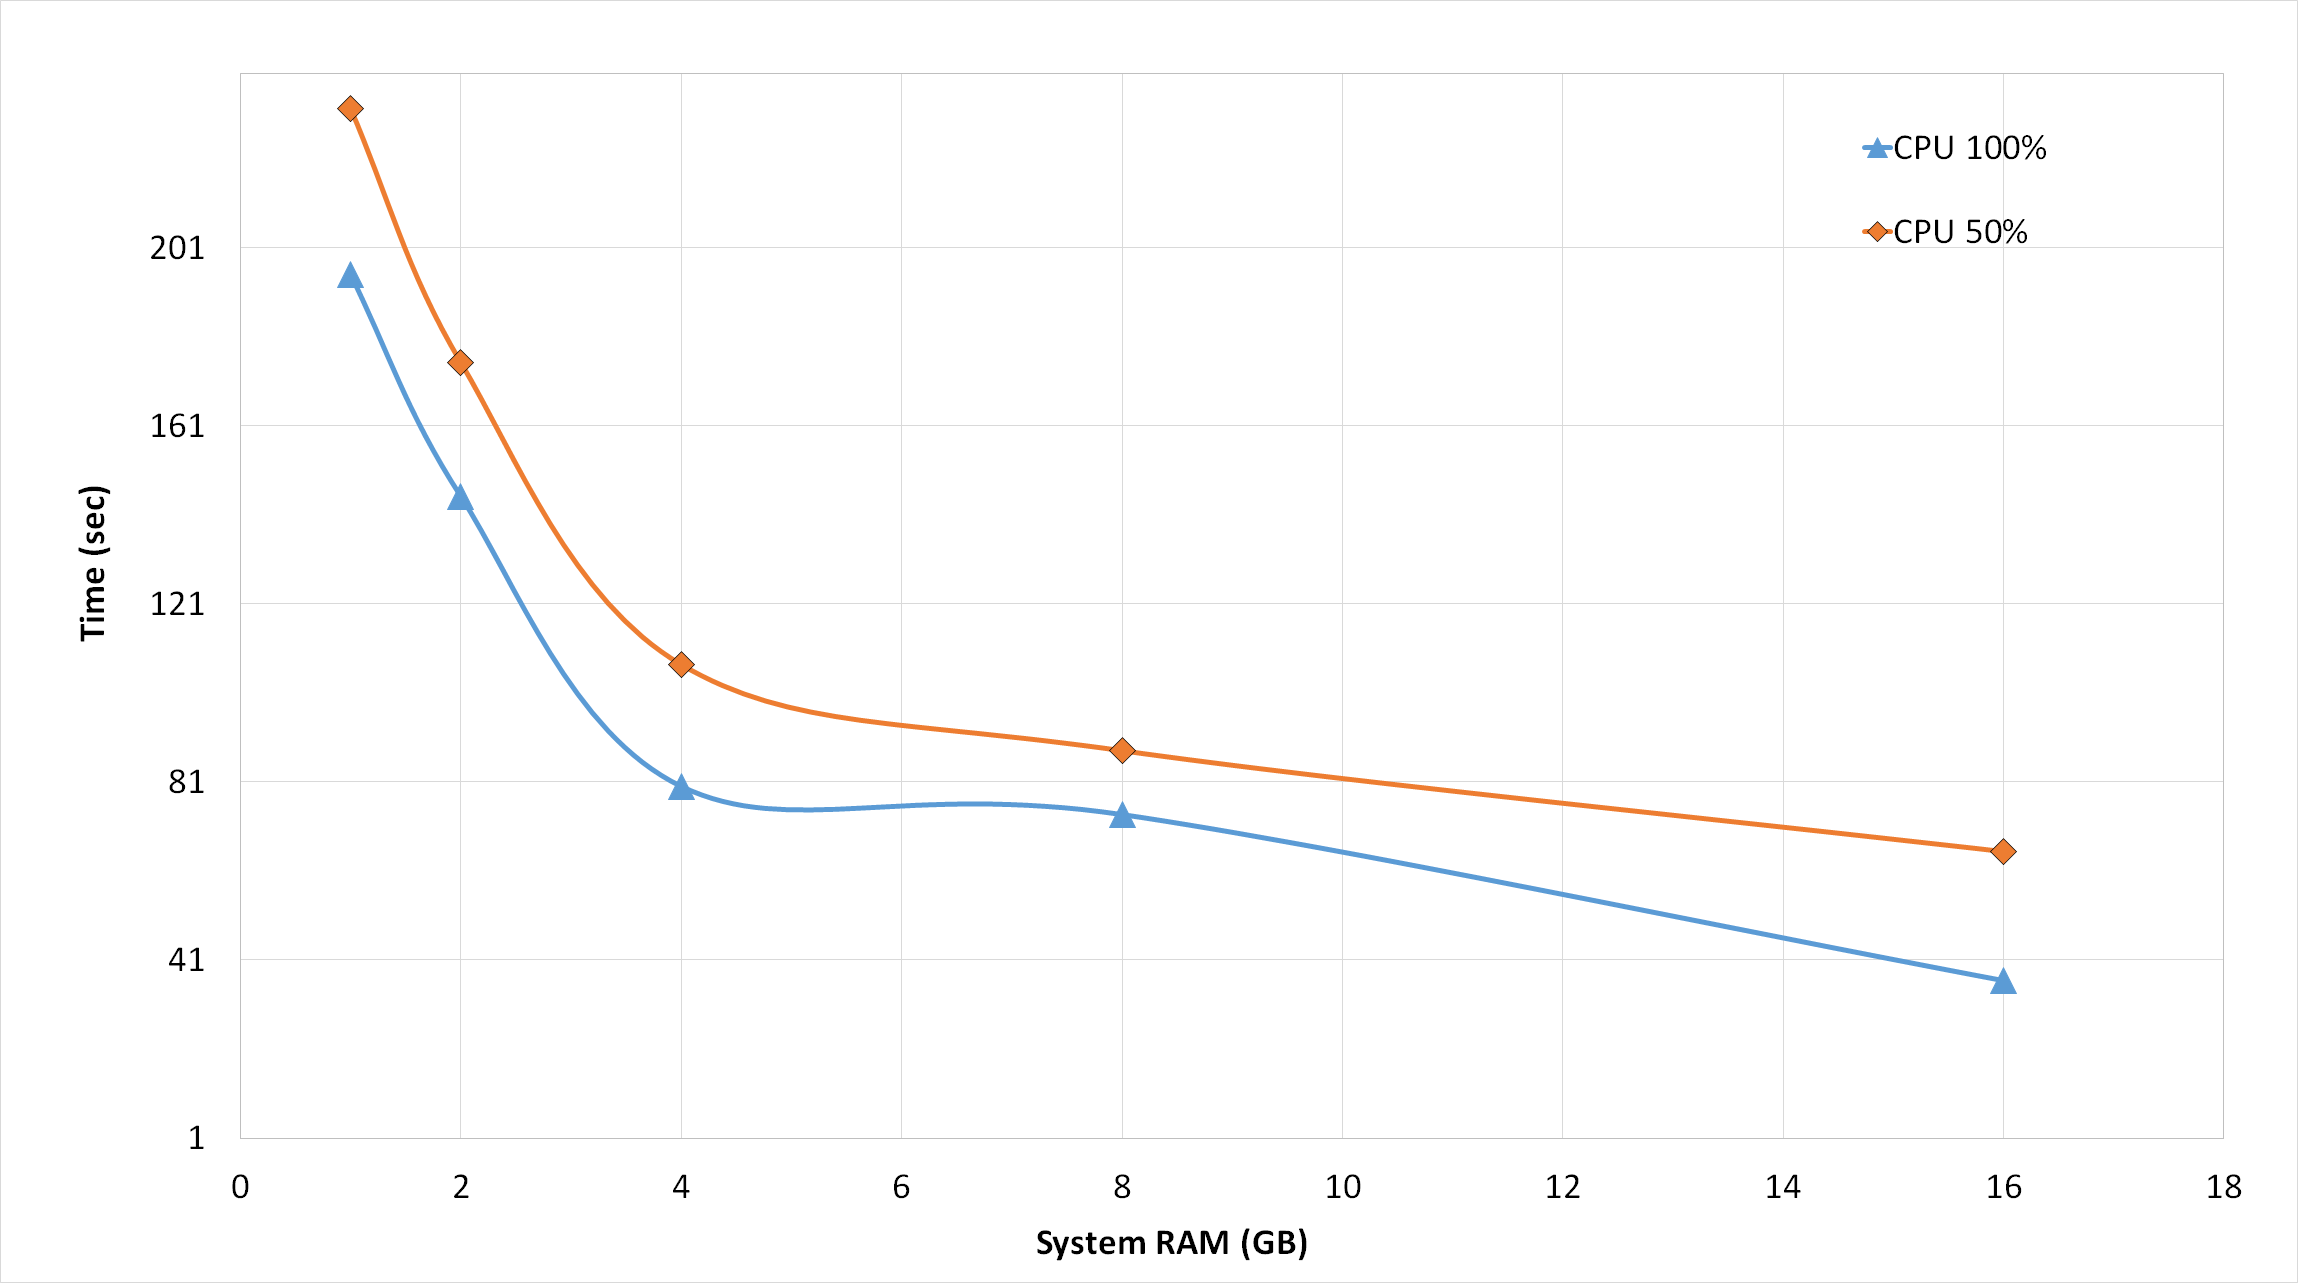
\includegraphics[width=1\textwidth]{Effect_of_System_resources_on_rate_of_consensus__2_.png}
\caption{Effect of System resources on block creation time}
\label{graph}
\end{center}
\end{figure}

It can be observed, from both Table 7 and Figure \ref{graph}, that the time to create a block gradually increases when the resources are limited. The lowest configuration that was tested here had a memory of 1 GB  with a 50\% of CPU Quota of the original physical machine. One point to be noted here, is that every Docker container was run on one CPU core every time. This limited the resources to an even greater extent. For example, in this case, the lowest resource configuration device could be a mid range Android phone or a tablet. Thus, a simple mobile device could potentially be the miner in this instance. However, as the size of the blockchain increases, it would be more and more difficult for a mobile device to be able to store it. A solution to that could be to offload the data onto a cloud server. As the number of miners grow in the blockchain, the difficulty level for a block to be generated would increase as well. The increase in difficulty level would, in turn, lead to more investment of computing resources of the device.

\subsection{Security Analysis} \label{Section: Security Analysis}
This section analyses some of the weaknesses associated with the security of blockchains in general as well as the proof of concept system. 

\subsubsection{Malicious Clients}
A client that does not follow the rules of a given blockchain network is no more considered a peer by all other clients, and ends up making another parallel blockchain with its own rules. A more malicious client that is able to pretend to follow rules of the blockchain system might possibly be able to act without getting noticed. 

In this case, there is a possibility that a manager, who also happens to be a miner, may go offline out of the blue, drop transactions, make wrong transactions, or even decline that a transaction ever happened. One way the system can circumvent this kind of behaviour is by using some more financial incentive for the managers to submit the correct information in all situations. As a miner, even if a manager refuses to verify transactions or declines that a transaction ever happened, the other mining nodes make up for it. The transaction can only be excluded if a majority, i.e. greater than 51 \% of the miners decline to include it. In general, the managers are assumed to be parties that the constrained devices trust, presumably the owners of those devices. Therefore, there should be no reason for the managers to want to sabotage the devices. The main advantage of using blockchains, as far as device management is concerned, is to ensure the data integrity. This makes sure that the data already in the system has not been modified - neither intentionally nor by accident. 

\subsubsection{Malicious External Smart Contracts}

In the case of smart contracts, any code that makes calls to an external smart contract is a potential security risk which has to be evaluated very carefully, specially if it includes some payment.  The following paragraphs explain some known attacks that can happen while making use of external contracts.

\paragraph{Denial of Service Attack}
The depth of the stack meant for making calls through the Ethereum Virtual Machine is limited to 1024. If an attacker continues making recursive calls until the stack depth limit, they may be able to take control of the smart contract code. This is called as the \textit{Call Depth Attack}\cite{ethereum-safety}. The attacker can also manipulate the amount of gas needed for a transaction and at the very least can make the gas required more than the block gas limit, thereby blocking any transaction from happening at all. 

\paragraph{Reentrancy}
One of the major security hazards of invoking an external contract from any given smart contract S, is that the external smart contract can make changes to its data without S having any idea. In this attack, functions of S are called over and over even before the first function call is finished. This may cause the different invocations of the same function to interact with each other in destructive ways \cite{ethereum-safety}. A way to tackle this problem is to treat the function that invokes the untrusted smart contract as an untrusted function itself. Another way to approach this would be to use a \textit{mutex} to lock a state in the function which can be unlocked by the owner of the lock alone. 

\subsubsection{Sybil Attack}
Many distributed systems do not have any form of identity management other than having accounts. Due to this reason, any actor is capable of creating multiple accounts. A Sybil Attack \cite{sybil} manifests when one actor can manage to act as multiple entities at the same time. An attacker can try to fill the network with the clients it controls. In such a case, the attacker can refuse to relay certain blocks or only relay the ones created by the attacker. 

A known solution to this attack is using a resource based counting mechanism, i.e., keeping a track of the accounts created per resource. Another approach to solving this can be to require the participants of the network to have a stake of a limited resource, such as cryptocurrency, so that they do not get any benefit out of pretending to be multiple entities in parallel. Manual authorization of each identity could also be a way, although tedious and inconvenient.

\subsubsection{Timestamp Hacking}
Each node maintains an internal counter representing the network time based on the median time of its peers. This information is exchanged between the nodes during peer connection. However, if the difference between the median time and the system time is greater than 70 minutes, the network counter time is set as the system time. An attacker could potentially affect the network time if it chooses to, by connecting multiple peers and reporting the time wrongly. This can be fixed by changing the network time calculation methodology done by the nodes\cite{bitcoin-weakness}.

\subsection{Limitations of the system}
The following paragraphs analyse some of the limitations of the proof of concept implementation. 

\subsubsection{Block creation time}
One disadvantage of the implementation is the amount of time it can take to create a block. As per Ethereum implementation, it may take up to 12 seconds to create a block in a public blockchain. Every time a transaction takes place in the blockchain, it goes into the queue to be picked up by a miner. This means waiting for a miner to collect transactions and then generate a new block. 

The block creation time issue is hard to avoid, given the nature of the Ethereum blockchain. This could pose a problem for the IoT devices in case of urgent access requirements. If the transaction difficulty is set low enough, the block creation time become relatively short. However, low difficulty could lead to multiple security issues as well as generation of more orphan and stale blocks.

\subsubsection{Changes to the system}
The transactions work based on the logic provided in the smart contract. If a change is to be made to the logic, or the way transactions are handled, the entire system has to be somehow set up from scratch. This would cost a lot of gas, not to mention other overheads such as the clients having to adapt to a new system. Another problem that arises from this is the access data getting lost, due to the smart contract system being set up all over again. 

To remedy this problem, distributed databases such as Swarm\footnote{Swarm: A decentralised content distribution platform. More information at http://swarm-gateways.net/bzz:/theswarm.eth/} or IPFS\footnote{IPFS: A peer to peer distributed web storage system. More information at https://ipfs.io/} can be made use of. This would mean that the actual data would be stored in these distributed databases instead of the smart contract memory. These distributed databases generate a hash based on the data stored in them. This hash, in turn, would be saved in the blockchain, thereby making it immutable. 

Therefore, in other words, if there any changes are required to be made to the system, there can be two possible approaches. Either a new smart contract needs to be written with the new logic or, a new smart contract that manipulates the existing smart contract needs to be created.


\subsubsection{Timestamp Dependence}
The system uses \textit{Block number} and \textit{average block time} to schedule the expiry of a specific rule. This is not definite as the block times may change with different releases of Ethereum.  
\newpage

\section{Discussion}
The aim of the thesis was to investigate how to securely manage IoT devices in a more autonomous and distributed way, without having to trust a central entity. The questions the thesis attempts to answer are as follows.
\begin{enumerate}
\item \textit{Is it possible to implement IoT device management, specifically in constrained devices, on blockchains, on a global level?}\newline

It has been found from the observations and experiments conducted during the course of this thesis, that Blockchain Technology has the potential to be utilised to authenticate device identity, protect and store data, handle access to devices, and process transactions in the operation of those devices, in a distributed way. The distributed replication model of blockchains facilitates accessing and supplying IoT information for customers as well as organisations, without requiring a centralized management server. The blockchain can also be used to securely make payments for services or use of device resources given pre-agreed conditions are tracked. 

\item \textit{What advantages does the use of blockchain bring to IoT?}

\subparagraph{Equal stakes} Blockchain technology has already proven its worth in the financial industry through the use of cryptocurrencies such as bitcoins. This concept can be adapted to fit the needs of IoT networks, thereby allowing billions of devices to talk to each other over the same network without the need for additional resources. Blockchain also takes into account the issue of ownership and authority between various vendors by ensuring everybody involved has equal stakes.

\subparagraph{Transparency, Privacy, Non-repudation, Integrity} The main advantage of using blockchains in IoT, is that it is public and transparent i.e., anybody participating in the blockchain network will have the chance to see all the transactions taking place and the blocks. At the same time, the complete transaction data is not visible. The involved parties in the transaction remain private since they transact under their respective accounts, and their personal information is protected by their private keys. This combination of non-repudiation and confidentiality helps improve the privacy aspect of blockchain transactions. Blockchain technology also incorporates hashing, which helps check the integrity of the information stored in the blockchain.

\subparagraph{Decentralization, Trustless} As blockchain is decentralized, there is no single central entity involved in approving transactions or set conditions for certain transactions to be accepted. This means that it is a highly trustless network, and requires consensus among all the participants in the network to accept transactions.

\subparagraph{Immutable} Most importantly, it is secure from the point of view that the data once entered cannot be changed, and may act as the single source of truth. This property of immutability is a major advantage of the blockchain technology. There is a possibility however, for a malicious node to try to change the data or deny that a transaction happened. But in such a case, the malicious miner would just be left behind, or desynchronise from the network and in turn would end up running its own tiny blockchain network which would be of no use to it.

\paragraph{Circular Economy} Another advantage the use of blockchain can bring to IoT can be to help build a so called circular economy\footnote{A circular economy is an economic model which focuses on reusing materials and value.}, where device resources can be shared instead of purchasing and disposing. 

\paragraph{Data Tracking} The ability to track the data exchange history corresponding to every single IoT device from the ledger of transactions, is also an important implication and is highly advantageous if used judiciously. 

\item \textit{What are the caveats and challenges of using blockchains for management processes in constrained devices, specially considered at a global perspective, and how can they be mitigated?}\newline

There are some shortcomings to using blockchains for IoT, but the solutions for them are either actively being worked on, or have already been solved at the time of writing the thesis. 

\paragraph{Storage Scalability}
One of them, is the issue of \textit{Scalability}. There are different factors that could come under the umbrella term of scalability. It includes aspects such as bootstrap time, transaction costs, throughput, latency time \cite{scalability}. \textit{Bootstrap time}, refers to the time taken by a new full node to completely synchronize with the blockchain. At present, Bitcoin has more than 100 GBs worth of data that new nodes might need to download and process in order to synchronize, and depending on the hardware specifications it takes an average of \textit{four days} to do so. \textit{Latency} refers to the maximum time taken to confirm a transaction, and \textit{maximum throughput} refers to the maximum rate at which the confirmation of transactions can be done on the blockchain. \textit{Transaction costs} comprise of the cost of \textbf{resources consumed} in order to have a confirmed transaction. This includes the digital currency paid as a transaction fee, as well as the physical currency paid for the operational costs of the hardware that acts as a node, bandwidth of the network and storage costs.

\paragraph{Energy consumption} 
When a cryptocurrency is in its nascent stage, the resources required to mine the currency do not amount to much. But as the difficulty level of mining the cryptocurrency increases, the miners need to resort to much more powerful hardware, and as we know, the more operational efficiency a hardware has, more energy it consumes. With the growth in mining farms all around the world, blockchain mining has very little regard for sustainability.

\subsubsection*{Mitigation Strategies for Scalability}
\subparagraph{SPV nodes}
As discussed earlier, SPV nodes download a copy of the headers of all blocks instead of the entire blockchain. This means that the storage requirements scale linearly with time, the start time being when Bitcoins were created, in this case \cite{bitcoin}. 

\subparagraph{Block Pruning}
As mentioned earlier in Section 2.1.6, the blockchain grows larger every 10 minutes. \textit{Block pruning} removes transactions that are no longer needed to verify if the blockchain is in a consistent state, and hence, allows full nodes to free up storage space \cite{bitcoin}. In terms of scalability, pruned nodes scale in the same way as the number of UTXO, or unspent transaction outputs. This means that the storage will scale O(n) where n is the number of users instead of number of transactions. 

\subparagraph{Sharding}
The main idea of \textit{sharding}\cite{shard}, is to split the memory address spaces of all the blockchain accounts into subspaces. For example, a sharding method can insert the accounts with addresses beginning with 0x00 into one shard, and addresses beginning with 0x01 into another one, and so on. Essentially, each shard has its own transaction history and the effects of state transitions corresponding to a particular shard is limited to that shard only. The effect of a transaction taking place in a particular shard though, will depend on the events taking place in the blockchain as a whole. Figure \ref{sharding} explains sharding with a simple example. 

Let us consider that account A, in shard X wants to transfer 100 digital coins to account B, in shard Y. In this case, the transaction taking place in shard Y depends on the events that took place previously in the other shard X. The 'debit' transaction in shard X destroys coins in that shard, whereas the 'credit' transaction taking place in shard Y creates coins in that shard, thereby showing how the legitimate transaction will take place.

\begin{figure}[H]
\begin{center}
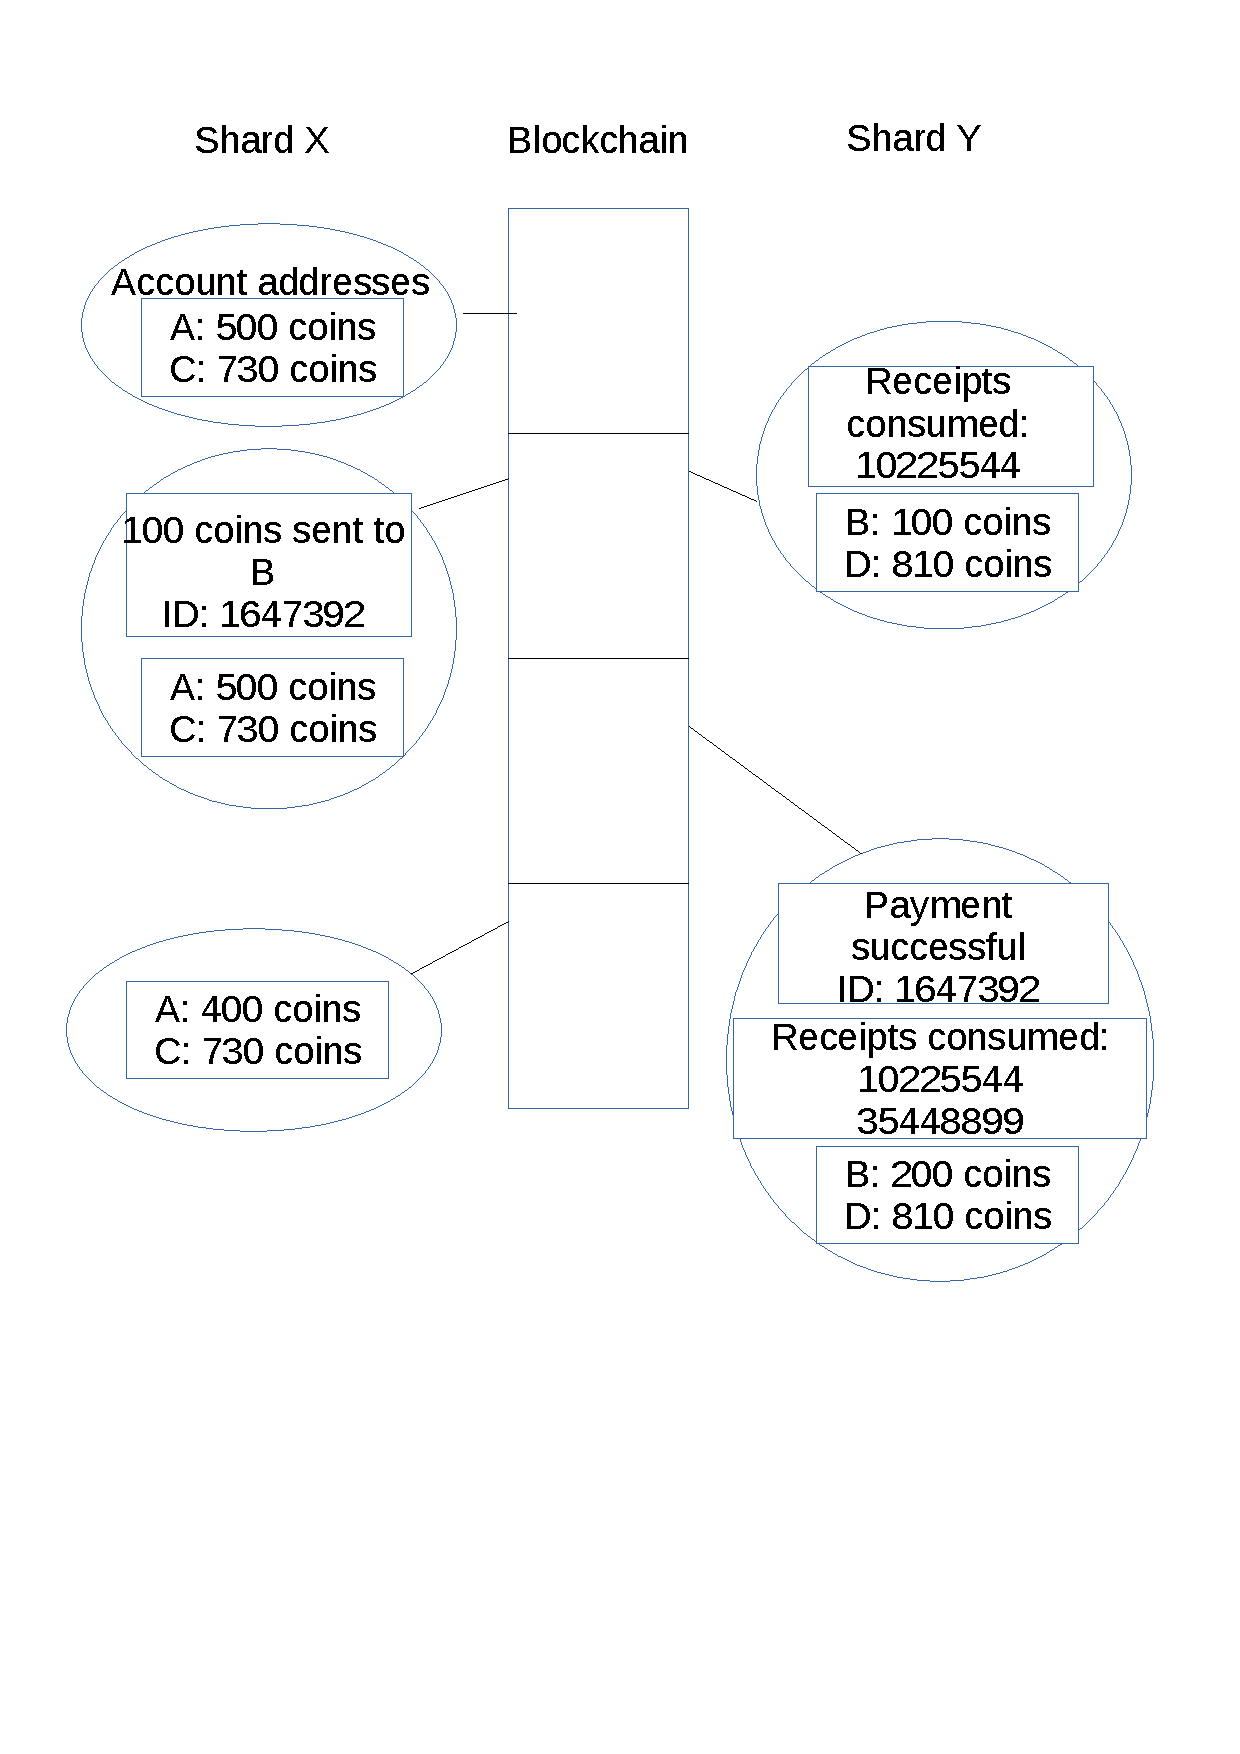
\includegraphics[width=0.6\textwidth]{cropped_Sharding.pdf}
\caption{Example: Sharding}
\label{sharding}
\end{center}
\end{figure}

Sharding is made use of commonly in distributed systems such as MongoDB, MySQL and BigDB.

\subparagraph{Scalable Blockchain Protocols}
\begin{itemize}
\item \textbf{BitcoinNG}\cite{bitcoinng}
The main problem BitcoinNG aims to solve is the improvement in transaction throughput and latencies in the blockchain, at the same time reducing the transaction confirmation to a few seconds. This protocol improves performance by decoupling Bitcoin's blockchain operations into two different planes namely, serialising transactions and electing a leader. The inventors of the protocol, divide time into epochs. A chosen leader is responsible for serialising state machine transitions, in every epoch. The leader is also responsible for creating new blocks in order to facilitate state propagation. Therefore, there are two kinds of blocks in this protocol, i.e., a key blocks, that elect the leader, and microblocks, that record the transactions.

BitcoinNG exhibits that the scalability of blockchain protocols can be improved until the only limiting factors are the individual node processing power, limiting throughput, and network diameter, limiting the consensus latency.

\item \textbf{Lightning Network}\cite{lightning}
The lightning network tries to address the issue of network scalability for blockchains. It uses the concept of \textit{micropayments} through payment channels for Bitcoin blockchains. Micropayments mean making small payments and receiving instant confirmations. The micropayments methodology allows two parties to open a payment channel for multiple payments and the actual transactions are recorded in the blockchain only after the channel closes. 
Without going into low level technical details of the protocol, it is necessary to bear in mind that this protocol mainly works with a minimal level of trust between two parties and keeps track of the channel time and whether the signatures for the transactions are properly done. The worst case scenario in this protocol is that one party keeps the funds of the other party locked for approximately a day. When the disadvantaged party opens a new payment channel, a refund is initiated since the other party had disappeared.  

\item \textbf{Bigchain DB} \cite{bigchaindb} is a blockchain database that claims to write one million transactions per second. All Bigchain DB nodes connect to a single ReThinkDB\footnote{ReThinkDB is a distributed, NoSQL database. More information at https://www.rethinkdb.com/} cluster. However, the flaw with the implementation is the failure to have independent storages. If the distributed database is attacked or if the blockchain has one malicious node that tries to delete the table, the entire system might be jeopardised. The other drawback to this blockchain database is the low performance of the interaction between the database and nodes connected to the blockchain.
\end{itemize}
  
\end{enumerate}
\newpage
\section{Conclusion}

The purpose of this thesis has been to study the blockchain system, and analyse if it is useful to employ the technology for identity and access management of constrained devices. A working proof of concept of an access management system was designed and implemented successfully on the Ethereum blockchain in order to assess the technology. This was done through extensive research and consideration of the choice of technology. The evaluation of the implementation proved that a blockchain based device management system may bring some advantage over the existing device management systems. Throughout the thesis, the advantages of using Blockchains have been revisited multiple times. 

The evaluation also revealed some limitations of the proof of concept system implemented, most of which were issues related to blockchain technology in general. The time it takes to generate a block, in particular, is a big disadvantage to a real time IoT setup, as the readings indicated. The issues of scalability, energy consumption, cost and block generation time were therefore examined in detail. It is essential for these issues to have a solution in order to have an even widespread adoption of the blockchain system. 

To conclude the thesis, despite the blockchain technology still being in early stages of development, it has many advantages that can be leveraged in a wide array of application domains. If the current challenges can be overcome, it can potentially change the way a lot of systems operate in the world.
\newpage
\section{Future Work}

In continuation with the current research, it would be interesting to see how the system would perform with physical nodes and real IoT devices. The current system uses \textit{Docker} containers to simulate a distributed blockchain environment, and just uses identification information of the constrained devices, since the idea was to first test out whether such a system is possible in the first place. An analysis of the data could determine the real world implications of the system to a certain extent. Therefore, an implementation of a full fledged hardware solution would be the most plausible next step.

In addition, it would be a good idea to include the suggested improvements for the system and develop a complete decentralized autonomous organization. This would lead to discovery of many more issues and challenges relevant to the system, in comparison with the controlled environment. 


\pagebreak
\nocite{*}
\bibliographystyle{tktl}
\bibliography{lahteet}

\lastpage

\appendices
\internalappendix{1}{Contract Creator function description}
\subsection*{Compile contract}
\textbf{Input}: Smart contract code in Solidity \newline
\textbf{Output}: Compiled version of the smart contract \newline

\textbf{Description}: This function uses the solidity compiler binding library for javascript. The smart contract code needs to be stored into a variable, without any line breaks, for this function to work. 

\subsection*{Calculate gas}
\textbf{Input}: The full transaction along with the data to be passed \newline
\textbf{Output}: The units of gas required to run the transaction\newline

\textbf{Description}: This function uses the \textit{estimateGas} method from the external \textit{Web3} javascript library, to determine the approximate amount of gas one needs to supply for the contract upload transaction to be successful.

\subsection*{Deployment format}
\textbf{Input}: The compiled smart contract code\newline
\textbf{Output}: Ready to deploy smart contract\newline

\textbf{Description}:
This function determines the \textit{ABI}\footnote{ABI: Application Binary Interface is a description of all the functions included in the solidity smart contract and how to use those functions.} of the smart contract, and encapsulates the compiled code into error handling blocks. It also takes care of other things such as having an unlocked user account for the deployment transaction, and checking if all the parameters required to upload the contract have been taken care of. It outputs the deployable version of the compiled smart contract code.
\subsection*{Deploy}
\textbf{Input}: Ready to deploy smart contract \newline
\textbf{Output}: Smart contract deployed on the blockchain\newline

\textbf{Description}:
This function deploys the smart contract that the previous function produced as an output, and outputs the smart contract address if successfully deployed.

\newpage
\internalappendix{2}{Smart Contract function description}
\subsection*{Manager Authentication Check}
\textbf{Input}: Manager's Ethereum address\newline
\textbf{Output}: True or False\newline

\textbf{Description}: It is a constant function that verifies whether the manager updating rules for a certain device in the smart contract memory is the one responsible for that particular device. It returns a Boolean value.

\subsection*{Query Manager}
\textbf{Input}: Manager's Ethereum address, Device's Ethereum address\newline
\textbf{Output}: True or False\newline

\textbf{Description}: This function takes the Manager and the constrained device addresses as inputs, and queries whether a certain Manager is responsible for a certain device or not. It returns a Boolean value. 

\subsection*{Query Rule}
\textbf{Input}: Manager's Ethereum address, Ethereum addresses of the two communicating devices\newline
\textbf{Output}: True or False\newline

\textbf{Description}: This function takes the Manager, and two constrained device addresses respectively as arguments. It queries whether a certain constrained device can access a particular constrained device or not. It returns a Boolean value.
\newline
\newline
\newline


\subsection*{Add Manager}
\textbf{Input}: Manager Ethereum address\newline
\textbf{Output}: True or False\newline

\textbf{Description}:
This function adds a manager in the smart contract memory on the blockchain. This function executes when a manager broadcasts an identitiy registration message, essentially making a call to the add manager function to add itself to the blockchain. It stores the manager address as a key value in a mapping, and returns a boolean value confirming if the add was successful. It also broadcasts a message on the blockchain claiming that the manager with the given address has been added. 

\subsection*{Add Device}
\textbf{Input}: Ethereum addresses of the Manager and Device\newline
\textbf{Output}: True or False\newline

\textbf{Description}: The manager of a constrained devices calls this function to add the particular device. It takes the manager address and the constrained device address as arguments, and adds the constrained device address in the value array corresponding to the key value mapped pair with the manager address as the key value. It then broadcasts a message over the blockchain indicating that the device corresponding to the specific manager has been added.

If the manager needs to add more devices corresponding to it, those addresses go into subsequent array indices in the value array of the key value pair. 

\subsection*{Add Rules}
\textbf{Input}: Ethereum addresses of the Manager and two communicating devices, Rule information\newline
\textbf{Output}: True or False\newline

\textbf{Description}: This function takes the manager's address, the constrained device's address that the manager manages, the new device's address that can now have access to the former device, the resources it can have access to, for how long the access is valid and what kind of access rights the latter can have over the former's specified resources. Access rights usually range between none, read and write indicated by numerical values, and the expiration time is specified by the number of blocks after which the access rights are expected to expire. The number of blocks is an indication of the time, in case of blockchains. After the data is stored in the smart contract memory, a message is broadcast to the blockchain indicating that a new rule has been added with the relevant details.

\subsection*{Remove Device}
\textbf{Input}: Ethereum addresses of the Manager and Device\newline
\textbf{Output}: True or False\newline

\textbf{Description}: This function takes the device address and the manager address as inputs and updates the value corresponding to the key value of manager address to zero. Then a message is broadcast over the network specifying the details of the device that has been de-registered from a particular manager on the blockchain.

\subsection*{Remove Rules}
\textbf{Input}: Ethereum addresses of the Manager and the two communicating devices\newline
\textbf{Output}: True or False\newline

\textbf{Description}: This function takes the constrained device addresses and the manager address as inputs and updates the value corresponding to the key value of constrained device address to zero. Then a message is broadcast over the network specifying the details of the rule that has been removed.

\subsection*{Remove Manager}
\textbf{Input}: Ethereum address of the Manager\newline
\textbf{Output}: True or False\newline

\textbf{Description}: This function takes the manager address as an argument. It first checks for any constrained device addresses corresponding to the manager as the key value. If there are none, it goes ahead with setting the corresponding value to null, and returns a true boolean value. Otherwise, an error is returned. This function also broadcasts a message over the network specifying the details of the manager that has been de-registered from the blockchain.

\subsection*{Execute Smart Contract Later}
\textbf{Input}: Expiration time specified as a rule information\newline
\textbf{Output}: True or False\newline

\textbf{Description}: This function takes the expiration time of a rule as the input. It then includes an internal logic to execute a transaction to the smart contract after the given expiration time, to update the rule description. A trusted external contract, called Ethereum Alarm Clock \footnote{Ethereum Alarm Clock: http://www.ethereum-alarm-clock.com/},  is also made use of to schedule the contract calling after the contract has expired.

\subsection*{Kill Smart Contract}
\textbf{Input}: Ethereum address of the contract creator\newline
\textbf{Output}: True or False\newline

\textbf{Description}: Only the creator of the smart contract has access to this function. This \textit{suicide} function was implemented in the prototype in the event of a bug or an unwanted behaviour that needs to be removed. 

\newpage
\internalappendix{3}{Client libraries used}
\subsection*{React}
React is a javascript library meant to create interactive user interfaces. The code of this library is mainly maintained by Facebook. It was used in the project to create the Client user interface. https://facebook.github.io/react/ 
\subsection*{Web3}
Web3 is a javascript library that communicates through RPC calls on a local Ethereum node, and basically exposes the RPC layer to communicate with Ethereum directly. https://github.com/ethereum/wiki/wiki/JavaScript-API 
\subsection*{Solc}
Solc javascript library binds javascript code to Solidity compiler, thereby making it possible to compile the smart contract code and deploy it. It uses Nodejs internally to do so, and more information about it can be found at https://github.com/ethereum/solc-js.
\subsection*{Lodash}
Lodash is a javascript utility library that contains many inbuilt high performance functions such as iterating through a javascript object, searching in javascript objects, using properties from different javascript objects to form a new object, etc. https://lodash.com/
\end{document}


